\documentclass[print]{dissertation}% [print] for print mode
\usepackage{microtype}
\usepackage{csquotes}
\usepackage{courier}
% FIGURES
% \usepackage{xr}
\usepackage{hyperref}
\usepackage{graphicx}
\usepackage{rotating}
\usepackage{wrapfig}
\usepackage[rightcaption]{sidecap}
% \usepackage{epstopdf}
\usepackage[font={small, it},      % small caption size
labelfont=bf,                % bold "Figure"
labelsep=period]{caption}    % separate Figure from text swith period
\usepackage[section]{placeins} % always place figures in section

% CHEMICAL FORMULAS
\usepackage[version=3]{mhchem} 	% Formula subscripts using \ce{}
\usepackage{chemformula}

% PHYSICAL UNIT FORMATTING
\usepackage[separate-uncertainty = true,
detect-all = true,
range-phrase = --,
range-units = single,
list-units = single,
multi-part-units = single]{siunitx}
\DeclareSIUnit[number-unit-product = {}]\uL{ \micro\liter}
\DeclareSIUnit[number-unit-product = {}]\fL{ \femto\liter}
\DeclareSIUnit[number-unit-product = {}]\umol{ \micro \mole}
\DeclareSIUnit[number-unit-product = {}]\mM{ \milli M}
\DeclareSIUnit[number-unit-product = {}]\uM{ \micro M}
\DeclareSIUnit[number-unit-product = {}]\nM{ \nano M}
\DeclareSIUnit[number-unit-product = {}]\pM{ \pico M}
\newcommand*\me[1]{\ensuremath{\bar{#1}\,}}

% MISC
\newcommand{\squeezeup}{\vspace{-2.5mm}}
%=============== extra: martin binfree =====================
% preamble:
\usepackage{mathrsfs}   % for laplace simbol
\usepackage{verbatim}   % useful for program listings
\usepackage{bm}% bold math
\usepackage{color}      % use if color is used in text
\usepackage{upgreek}
\newcommand{\ve}[1]{{\mathbf{#1}}}

\begin{document}

%%%%%%%%%%%%%%%%%%% MAIN PART %%%%%%%%%%%%%%
\title[]{Fluorescence of Single Copper Proteins: Dynamic Disorder and Enhancement by a Gold Nanorod}
\author{Biswajit}{Pradhan}

\frontmatter
 \begin{titlepage}

\begin{center}

% %% Extra whitespace at the top.
% \vspace*{2\bigskipamount}

% %% Print the title.
% {\makeatletter
% \titlestyle\bfseries\LARGE\@title
% \makeatother}

% %% Print the optional subtitle.
% {\makeatletter
% \ifx\@subtitle\undefined\else
%     \bigskip
%     \titlefont\titleshape\Large\@subtitle
% \fi
% \makeatother}

% \end{center}

% \cleardoublepage
% \thispagestyle{empty}

% \begin{center}

%% The following lines repeat the previous page exactly.

\vspace*{2\bigskipamount}

%% Print the title.
{\makeatletter
\titlestyle\bfseries\LARGE\@title
\makeatother}

%% Print the optional subtitle.
{\makeatletter
\ifx\@subtitle\undefined\else
    \bigskip
    \titlefont\titleshape\Large\@subtitle
\fi
\makeatother}

%% Uncomment the following lines to insert a vertically centered picture into
%% the title page.
%\vfill
%\includegraphics{title}
\vfill

%% Apart from the names and dates, the following text is dictated by the
%% promotieregelement.

{\Large\titlefont\bfseries Proefschrift}

\bigskip
\bigskip

ter verkrijging van de graad van doctor

aan de Universiteit Leiden,

op gezag van de Rector Magnificus prof.~mr.~C.~J.~.J~.M~.Stolker,

voorzitter van het College voor Promoties,

in het openbaar te verdedigen op dinsdag 3 april 2018 om 15:00 uur

\bigskip
\bigskip

door

\bigskip
\bigskip

%% Print the full name of the author.
\makeatletter
{\Large\titlefont\bfseries\@firstname\ {\titleshape\@lastname}}
\makeatother

\bigskip
\bigskip


geboren te Odisha, India \\
in 1991

%% Extra whitespace at the bottom.
\vspace*{2\bigskipamount}

\end{center}

\clearpage
\thispagestyle{empty}

%% The following line is dictated by the promotieregelement.
\noindent Promotors:

%% List the promotors (supervisors).
\medskip\noindent
\begin{tabular}{l}
    Prof.\ dr.\ M.\ Orrit \\
    Prof.\ dr.\ G.\ Canters
\end{tabular}

% List the (optional) copromotor.
\medskip
\noindent Copromotor: Prof.\ dr.\ T.\ Aartsma

\medskip
\noindent Promotiecommissie:

%% List the committee members, starting with the Rector Magnificus and the
%% promotor(s) and ending with the reserve members.
\medskip\noindent
\begin{tabular}{ll}
    Dr.\ K.\ Blank (Max Planck Munich) \\
    Dr.\ P.\ Zijlstra (Technische Universiteit Eindhoven) \\
    Prof.\ dr.\ ir.\ S.J.T. van Noort \\
    Prof.\ dr.\ E.R.\ Eliel \\
    Prof.\ dr.\ E.J.J.\ Groenen \\
    Prof.\ dr.\ A.\ Kros \\
\end{tabular}

%% Include the following disclaimer for committee members who have contributed
%% to this dissertation. Its formulation is again dictated by the
%% promotieregelement.
% \medskip
% \noindent Prof.\ dr.\ ir.\ J.\ Doe heeft als begeleider in belangrijke mate aan de totstandkoming van het proefschrift bijgedragen.

%% Here you can include the logos of any institute that contributed financially
%% to this dissertation.
\vfill
\begin{center}
    
\includegraphics[height=0.8in]{frontback/logos/leiden}
    \hspace{2em}
    
\includegraphics[height=0.8in]{frontback/logos/casimir} \\
    \includegraphics[height=0.8in]{frontback/logos/fom}
%    \hspace{2em}
%    \includegraphics[height=0.5in]{title/logos/nwo}
\end{center}
\vfill

\vspace{4\bigskipamount}

\noindent Copyright \textcopyright\ 2018 by B.~Pradhan

%% Uncomment the following lines if this dissertation is part of the Casimir PhD
%% Series, or a similar research school.
%\medskip
%\noindent Casimir PhD Series, Delft-Leiden 2013-01

\medskip
\noindent ISBN 000-00-0000-000-0

\medskip
\noindent An electronic version of this dissertation is available at \\
\url{http://repository.tudelft.nl/}.

\end{titlepage}


\tableofcontents
\mainmatter

% %========== CHAPTERS ================
\thumbtrue
\chapter{Introduction}
\label{chapter:intro}
\graphicspath{{./chapters/c1_intro/figures/}}
%=========== MAIN ================
This chapter contains the basics needed for the work done in this thesis.
Towards the end of this chapter, an overview of all the chapters is given.
%============== MAIN ================
\section{Fluorescence}
The absorption and subsequent emission of light by materials is called fluorescence.
The term Fluorescence was named by \textit{George Gabriel Stokes} after observing ultraviolet light being transformed into visible light in the mineral fluorite.\cite{Stokes1852}
A molecule is excited to a higher electronic energy state after absorbing a resonant photon.
Each electronic energy level is associated with vibrational and rotational energy levels.
The excess vibrational energy gained in the excited state is quickly lost to the surrounding in a time period of sub-picoseconds and the molecule stay in its zero vibrational level of excited state for about nanoseconds..
If it allowed to come down to the ground state which is decided by the spin states (singlet allowed) of the paired the electrons and Franck-Condon principle, \textit{fluorescence emission} is observed.
The emitted photon has a smaller energy than the absorbed photon leading to Stoke's shift and the total time it takes to come down to the ground state is called fluorescence lifetime typically \SI{10}{\ns}.
If the system crosses over from singlet excited to the triplet state, emission may be observed at even longer wavelength and even longer lifetime which is known as \textit{phosphorescence}.
The processes between the absorption and the emission is normally represented graphically by Jablonski diagram.
\begin{figure}
	\centering
	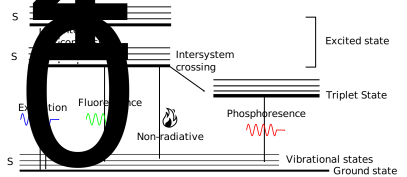
\includegraphics[width=0.8\textwidth]{jablonski}
	\caption{\textbf{Jablonski Diagram}}
	\label{fig:jablonski}
\end{figure}

Natural materials that show fluorescence include minerals, tissue in plants and animals.
Among biological molecules nicotinamide adenine dinucleotide (NADH), flavins (FAD), chlorophyll are abundantly found fluorescing.
Extrinsic fluorophores are also synthesized with high quantum yield and varying color which include synthetic dyes, quantum dots.
Fluorescence has a huge advantage of very low background which enables their detection with very low concentration of fluorescent molecules.
This was very important for biological imaging as little quantity of such markers keep the system under study unaffected.
Not only external fluorophores can be used for biological marking, the cells can also be gene-edited to produce their own fluorophores called fluorescent protein (GFP).
Now a days it is unthinkable to use a biology or analytical chemistry lab without fluorescence technique.

\section{Single Molecule Spectroscopy}
The thought experiment by Jean Perrin to observe single fluorescent molecules was materialized for the first time in 1990s at extremely low temperature and in an advanced laboratory.\cite{orrit1990single}
The rapid development of optical microscope, lasers, dyes and detectors now made it possible to detect single molecules at room temperature on a bench top.\cite{xie1998optical,weiss1999fluorescence,moerner1999illuminating}
Not only it has grown itself into an important research field, the concept is now heavily used in molecular biology, super-resolution microscopy, quantum computing, catalysis to name a few.\cite{zhuang2000a,huang2008threedimensional,eisaman2011invited,lounis2005singlephoton,roeffaers2007singlemolecule}
The following advantages provided by single-molecule study makes it an indispensable technique:
\begin{itemize}
	\item \textbf{No averaging.} Ensemble measurements provide mean value of a physical quantity, looking at average behavior of vast number of molecules.
	In complex medium like in condensed matters and cellular matrix, each molecule is in a different microscopic surrounding experiencing different forces and resistances.
	Single molecule measurements provide distribution of quantities distinguishing the subpopulations within the system with similar characteristics.
	For example different host molecules even in a crystalline (ordered structure) solids shows different spectral lines and line widths discovering the imperfections.\cite{kozankiewicz1994single,reilly1993spectral}
	Small domains of \SIrange{50}{700}{\nm} in a cell membrane are located based on the difference in their diffusion coefficient.\cite{lommerse2004singlemolecule}
	Rare species that are lost in ensemble measurements can be identified and investigated in SM studies.
	The distribution in spatial dimension is called static heterogeneity.
	\item \textbf{Time dependent fluctuation.} Dynamics of systems can be studied without the need for synchronization (kinetic measurements in ensemble often require synchronization).
	Single molecule measurements at equilibrium provide direct access to both dynamics and statistics of molecular complexes.
	They also provide information on a wide range of time scale from microseconds to tens of seconds extracting translational, orientational, enzymatic-turnovers and protein folding-unfolding events.
	\item \textbf{Local reporter} As single molecule detection is based on optical microscopy, the observer can be far away from the molecule itself provided the intervening medium is optically transparent.
	The trajectory of the reporter molecules deep inside the cell can be tracked to follow the activities of the host.
	\item \textbf{Tool.} Single-molecules are finding their ways to be used tools to perform different tasks.
	As the transitions in the excitation of single-molecules are quantum in nature, they can be used as pure source of single photons for quantum computing.
	The single step blinking nature of single molecules has been used for super localization and there by spatially differentiating up to nanometer scale.
	Moerner, Betzig and Hell were awarded Nobel prize in Chemistry in 2014 for their contribution towards super-resolution microscopy and single-molecule detection.
\end{itemize}
Here we discussed some of the applications of Single-molecule measurements which provide plethora of information and the possibilities are only limited by the practitioner's creativity and imagination.

Two major characteristics that proves the detection of Single molecules are their stepwise changes of intensity and anti bunching.
Molecules in their excited state can cross over to triplet state resulting in loss of emission until the molecules comes back to the ground state to keep the excitation-emission cycle going.
This results in blinking of intensity between two levels.
A molecule on the triplet state is more reactive because of its unpaired electrons and can react with triplet oxygen in the system leading to bleaching and complete loss of fluorescence.
Both one step blinking and bleaching information can be used to identify single molecules.
Single molecules are quantum systems that can only emit one photon at a time.
When the photon stream from the molecule is sent to two detectors via a beam splitter, anti bunching is observed in the autocorrelation of the two spitted signals.
Such anti bunching experiments to determine the singleness of the photon source is known as ``Hanbury-Brown Twiss  measurement''.
\begin{figure}
	\centering
	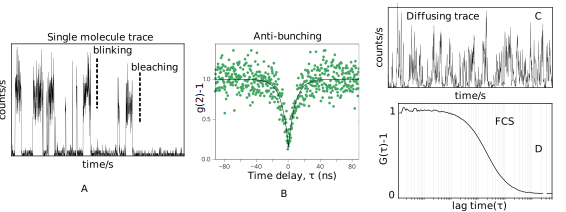
\includegraphics[width=\textwidth]{SM_characteristics}
	\caption{\textbf{Single-molecule characteristics.}
	(A) Time trace of a single molecule showing single-step switching (blinking) and bleaching.
	Notice the reappearance of the intensity after blinking but complete disappearance after bleaching.
	(B) Anti-bunching at zero delay time in the correlation shows the singleness of the emitter.\cite{chu2016a}
	(C) Time trace of diffusing molecules in a fluid with \SI{1}{\nM} fluorophores showing intensity bursts and the correlation amplitude ($G(\tau)-1={\sim}1$) indicates the presence of few molecules in the focus.}
	\label{fig:SM_characteristics}
\end{figure}

Fluorescence correlation spectroscopy (FCS) also considered as a single-molecule technique, measures the temporal correlation of fluctuating light intensities.
Conventional way to perform FCS is to collect signal from \textit{diffusing fluorescent} molecules in the diffraction limited focal volume and then compute the autocorrelation of the intensity trajectory.
The autocorrelation of the intensity signal is given as $G(\tau)=<I(t)I(t+\tau)>/<I(t)>^2$ where I is the intensity, $\tau$ the lag time and $<...>$ represents time averaging.
The correlation quantifies the probability the intensity at time $t$ is similar to the intensity at a later time $t+\tau$.
It provides information on the concentration and the time scale of the fluctuating observable.
By very nature, FCS technique require the fluctuation of the number of diffusing fluorophores in the diffraction limited volume of \SI{1}{fL}, ideally one molecule in average which translates to a concentration of \SI{1}{\nM}.
Because of the diffraction limit ($\Delta{x}={\lambda}/2$), FCS is often limited to nanomolar concentration of the analyte. 

Two of the important requirements to measure single molecules with high spatial and temporal resolution are (i) high fluorescence yield and (i) small excitation and detection volume.
In this thesis we push the limit of single-molecule detection to low quantum yield dyes and to high concentration of fluorophore.
\section{TCSPC}

\section{FRET}
%
\section{Optical Nanoantennas}
\section{Gold nanorod surface plasmon}
\section{Fluorescence Enhancement by plasmonics}
%
\section{Enzymology and Electron transfer}
\section{Protein at work are Proteins in Motion}
\section{Azurin: a copper containing redox protein}
\section{Flurox Principle}
\subsection*{FRET as Redox state indicator}
%
\section{This thesis}

\chapter{Gold-Nanorod-Enhanced FCS of Fluorophores with High Quantum Yield in Lipid Bilayers}
\label{chapter:EFCS}

% \blfootnote{This chapter have been published in Journal Physical Chemistry C 2016, 120, 25996−26003.}
\graphicspath{{chapters/c2_bilayer_efcs/figure/}}
%==========abstract==========
\begin{abstract}
	Plasmonic fluorescence enhancement is used to study fluorescence correlation spectroscopy (FCS) at higher concentrations than in regular diffraction-limited FCS experiments.
	Previous studies suffered from sticking to the substrate and were performed mainly with poorly emitting dyes.
	A lipid bilayer forms a passivating surface preventing sticking of the dye or the protein and allows for specific anchoring of probe molecules.
	For dyes with high quantum yields, the fluorescence background of unenhanced molecules is high, and the fluorescence enhancementis weak, less than about 10.
	Nonetheless, we show that FCS is possible at micromolar concentrations of the probe molecule.
	Enhanced FCS is recorded by selecting signals on the basis of their shortened lifetime.
	This selection enhances the contrast of the correlation by more than an order of magnitude.
	The lipid bilayer can be used to anchor biomolecules and perform enhanced FCS, as we show for a dye-labeled protein.
\end{abstract}
\pagebreak
%============================Introduction=====================================
\section{Introduction}
Fluorescence-based single-molecule detection helps exploring the structure and dynamics of complex biological matter.\cite{moerner1999illuminating,weiss1999fluorescence}
Single-molecule signals can reveal a transient state during a chemical reaction, or report on the kinetics of processes as a function of position.
Broadly there are two ways of studying single molecules: i) by immobilizing the molecule on a backgroundfree matrix or surface,ii) by dissolving the molecules in a fluid and measuring the signal fluctuation by fluorescence correlation spectroscopy (FCS).\cite{Magde1972}
Both techniques require the molecule to possess a high quantum yield and good photostability.
FCS studies are limited to concentrations in the pico- to nano-molar range, in view of the diffraction-limited detection volume of a few femtoliters (fL).
As many biological reactions occur in the micromolar range\cite{craighead2006future}, smaller detection volumes are desirable to study these reactions by FCS.

Plasmonic nanostructures can both enhance molecular fluorescence in volumes smaller than the diffraction-limited volume and reduce the background fluorescence of the other molecules in the diffraction-limited volume.
Zero-mode waveguides and antennas-in-box, in particular, both enhance fluorescence and reduce background.\cite{levene2003zeromode,kinkhabwala2012fluorescence,punj2013a,yuan2013thousandfold,punj2013gold} 
The effective fluorescence enhancement depends sensitively on the position and orientation of the molecule with respect to the nanoparticle.
It originates from two factors, excitation enhancement and radiative enhancement.
By confining the optical field into so-called hot spots with volumes much smaller than the diffraction limit,\cite{schuller2010plasmonics} plasmonic nanostructures enhance the incident field by up to a few orders of magnitude, leading to excitation enhancement.\cite{yuan2013thousandfold,anger2006enhancement,kinkhabwala2009large,
acuna2012fluorescence,busson2012accelerated,holzmeister2014quantum,khatua2014resonant}
They also alter the radiative and non-radiative decay rates of molecules in their vicinity.
The ensuing radiative enhancement results from improved emission by the nanoantenna dipole induced by the molecular dipole.
In addition, energy may be transferred from the molecule to the antenna resulting in non-radiative losses and energy dissipation in the metal.
Changes in the radiative or non-radiative decay paths lead to altered, generally shortened fluorescence lifetimes.\cite{khatua2014resonant,liu2007quantized,lakowicz2001radiative,dulkeith2005gold,seelig2007nanoparticleinduced,muskens2007strong,pelton2015modified}
Distance-dependent lifetime measurements show lifetime shortening up to \SI{40}{\nm} away from the metal surface.\cite{seelig2007nanoparticleinduced}

Noble-metal plasmonic nanostructures can be fabricated either by lithography or by colloid chemistry.\cite{zijlstra2011single}
Whereas lithography can produce nanostructures with arbitrary geometries suitable for high optical confinement, it presents the disadvantages of complex processing, polycrystallinity, surface roughness, and high cost.
Colloidal chemistry produces large numbers of highly crystalline nanostructures in a few basic shapes (spheres, rods, bipyramids, etc.) that are controllable to some extent, at a low cost. 
Among the basic nanoparticle shapes, nanorods\cite{yuan2013thousandfold} can be just as efficient as lithographically-made structures\cite{punj2013a,kinkhabwala2009large} in enhancing fluorescence.
Gold nanorods confine the optical field more weakly than lithographically made gap structures, but they have the advantage of a narrow surface plasmon resonance, which can be tuned in the red and near infrared range by changing the rods\textquotesingle aspect ratio.\cite{khatua2014resonant}
The largest enhancement is achieved for a maximum overlap of the molecule\textquotesingle s excitation and fluorescence spectra, of the nanorod\textquotesingle s surface plasmon resonance, and of the excitation wavelength.
Further advantages of gold nanoparticles are that they provide easy access of hot spots to diffusing molecules and that they can be inserted into complex environments such as living cells.

Confinement of light in volumes much smaller than the diffraction-limited volume combined with fluorescence enhancement open applications of FCS at micromolar dye concentrations.
The correlation contrast in FCS decays as the square of the background intensity.
To reduce background, most enhanced FCS experiments have been done on dyes with low quantum yields.\cite{kinkhabwala2012fluorescence,estrada200810000}
Alternatively, a fluorescence quencher may be added to a dye with a high quantum yield (QY) to reduce background.\cite{punj2013a,punj2013gold}
A metal box or cladding\cite{ghenuche2015matching} can also be fabricated around the nano structure to improve the correlation contrast against the background of unenhanced molecules.
Both solutions have disadvantages, as a millimolar quencher concentration may be harmful to a living cell.
Metal claddings are difficult to fabricate and to manipulate in a complex environment.
Generalizing enhanced FCS to high-QY dyes would obviate these two problems and open plasmonic enhancement to biological marker dyes, most of which have high QY.
Plasmonic enhancement may also help overcome other background sources such as autofluorescence in live-cell experiments.
Indeed, as we show herein, even weak fluorescence enhancements suffice to overcome background in FCS experiments.
Moreover, fluorescence photons with short emission times may be selected as was done by Acuna et al\cite{acuna2012fluorescence} further to improve the signal to noise ratio of enhanced FCS.

A further limitation in working with metal nanostructures on a solid substrate is the nonspecific interaction of the molecules with metal and substrate, which not only may affect the molecules’ functionality but also make measurements troublesome.\cite{kinkhabwala2012fluorescence,yuan2013thousandfold,zhang2009gold}
Micellar solutions have been used to minimize sticking but are not ideal when studying biomolecules or performing experiments in live cells. 
We therefore need to suppress or mitigate nonspecific interactions of the dyes or biomolecules under study with the solid substrates supporting the structures.
Living organisms use a lipid bilayer on their outer surface to prevent nonspecific interaction and protein fouling while allowing specific binding of membrane proteins.\cite{zhang2009gold,cooper2000cell}
We have used a supported lipid bilayer to passivate the substrate.\cite{persson2012lipidbased,ller2012single,lohmuller2011supported}
Supported bilayer can be self-assembled on solid surfaces (glass, silica, and similar polar surfaces) such that it forms a single, 
continuous membrane which possesses a high degree of lateral mobility by maintaining a very thin layer of water (\SI{1}{\nm}) between substrate and bilayer.\cite{sackmann1996supported,CASTELLANA2006429,cremer1999formation,richter2006formation} 
Bilayers are also model systems to study diffusion in biological membranes.
In standard experiments, diffusion in bilayers is studied on length scales limited by far-field resolution. Plasmonic enhancement gives us access to diffusion on the length scales of the near field, typically some tens of nm.
Enhanced fluorescence experiments provide access to nanoscale diffusion in the vicinity of a gold nanorod.

Here we study fluorescence enhancement of a high-QY dye by immobilized single gold nanorods.
Sticking of the dye to the glass substrate was prevented by coating the glass with a supported lipid bilayer formed from a zwitterionic lipid.
We have characterized the properties of the enhanced signal and shown that its fluorescence decay is much faster than the far-field signal’s.
Based on these time decay characteristics, we have filtered the near-field signal from the background of unenhanced dye fluorescence, thereby obtaining an improved FCS contrast.
The same measurement provides both far-field and near-field diffusion components, and allows us to compare the diffusion kinetics in both regimes. 
We show that biomolecules can be successfully anchored in the bilayer, and that enhanced FCS can be performed while sticking and interaction with gold nanorods are prevented.
\begin{figure}
	\centering
	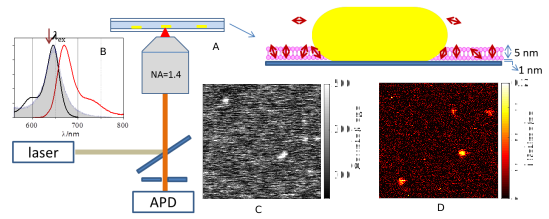
\includegraphics[width=\textwidth]{schematic_efcs}
	\caption{(A) Schematic diagram of the optical setup with a supported lipid bilayer (pink), ATTO 647N molecules (red) and a gold nanorod (yellow).
	(B) Absorption spectrum of ATTO 647N (black), fluorescence spectrum of ATTO 647N (red) and photoluminescence spectrum of a single gold nanorod (shaded area).
	Notice the overlap of the nanorod\textquotesingle s SPR with the dye\textquotesingle s absorption and emission spectra.
	(C) fluorescence intensity image (size $\SI{8}{\um}\times\SI{8}{\um})$ and (D) fluorescence lifetime image (FLIM) of the same area of 
	lipid bilayer. Note the lack of correlation between the fluorescent spots indicating dye aggregates in (C) and the short-lifetime spots in (D) indicating the rods.}
	\label{fig:schematic}
\end{figure}
%===========================Methods================================
\section{Methods}

\paragraph*{Gold nanorod immobilization.}
Gold nanorods (AuNRs) were synthesized in cetyl trimethyl ammonium bromide (CTAB) using the seed-mediated growth method.\cite{nikoobakht2003preparation}
The average dimension of the nanorods was $\SI{90}{\nm} \times \SI{50}{nm}$. Fig. S\ref{SIfig: AuNR_uv-vis}B shows a scanning electron microscopy image of the nanoparticles.
The bulk absorption spectra of these nanorods in Fig.S\ref{SIfig: AuNR_uv-vis}A show the longitudinal surface plasmon resonance (LSPR) 
at \SI{640}{\nm}. The nanorod sample was diluted and the CTAB was washed away by centrifugation and re-suspension in milliQ water before use.
Glass coverslips (Menzel-Glaser, \SI[product-units=repeat]{22x40}{\mm}, no. 1 thickness) were used for immobilization.
The coverslips were sonicated in water (\SI{15}{\minute}) and acetone (\SI{15}{\minute}).
Then they were rinsed in milliQ water several times and incubated in a \ce{H2O}/\ce{NH4OH}/\ce{H2O2} (5:1:1) bath at \SI{70}{\celsius}.
The coverslips were rinsed several times with water and ethanol, and finally stored in ethanol.
Before use the coverslips were flamed, and then ozone-cleaned for \SI{15}{\minute}.
The nanorods were spin-coated onto these coverslips at \SI{2000}{rpm} for \SI{1}{\minute}. 
These parameters gave us around 5 particles per \SI{100}{\um\squared} area and more than \SI{90}{\percent} of them were single. 
The coverslips with the gold nanorods were then rinsed with water to remove remaining traces of CTAB, dried, and again ozone-cleaned for \SI{30}{\minute}.
This resulted in a very  hydrophilic surface. The coverslip was mounted in a homemade flow cell, where the surface was further prepared for confocal experiments.

\paragraph*{Supported lipid bilayer preparation.}
Supported lipid bilayers were prepared from a zwitterionic lipid.
Stock ampoules (\SI{25}{\mg} ) of 1-palmitoyl-2-oleoyl-sn-glycero-3 phosphocholine (POPC, see Fig.Sref{SIfig:chemical}B) were purchased from Avanti polar and stored at \SI{-20}{\celsius} immediately after receipt.
The lipid powders were dissolved in chloroform and dried with argon in glass vials \SI{1}{\mg} each and again stored at \SI{-20}{\celsius} until required.
\SI{4}{\ml} of Phosphate Buffered Saline (PBS) were added to the glass vial and the POPC was incubated for \SI{1}{\hour} at \SI{40}{\celsius} (which gives a concentration of \SI{0.25}{\mg\per\ml}.
Then the vial was placed in the middle of a sonicator where the cavitation is greatest.
It was sonicated for \SI{30}{\minute} to produce small unilamellar vesicles (SUVs). 
The coverslips in the flow cell were hydrated by flowing PBS into the cell for \SI{5}{\minute}.
Then the coverslip was incubated with the SUV sample for \SI{1}{\hour} and washed with PBS to remove all free vesicles and debris.
The vesicles rupture, spread and form a bilayer.\cite{richter2006formation}
For protein anchoring, the vesicles for the bilayer were prepared from a mixture of POPC and DSPE-PEG(2000) Biotin (See Fig.S\ref{SIfig:chemical}C) with a ratio of 100:1.

\paragraph*{Labeling of the bilayer.}
ATTO 647N NHS-ester (see Fig. S\ref{SIfig:chemical} for the structure) was purchased from ATTO-TEC.
Before labeling, the reactive part of the dye (NHS-ester) was neutralized by incubating in \SI{20}{\mM} Tris buffer pH 9 (the amine group present in Tris reacts with the ester).
The dye in Tris pH 9 buffer at the concentration required by the experiment (vide infra) was passed into the flow cell.
The dye goes into the bilayer only at higher pH probably because of the neutralization of charge on the nitrogen atom present on the head group of the lipid molecules. 
The dye mentioned in the whole discussion is ATTO 647N unless otherwise stated.

\paragraph*{Protein to bilayer anchoring}
Wild type (wt) azurin was prepared, purified and labeled as previously described.\cite{VANDEKAMP1990283,nicolardi2012top-down}
ATTO 655 NHS ester was incubated with the azurin and azurin labeled at Lys122 was isolated and purified by chromatography on a MONO Q anion exchange column. 
Biotin-PEG-NHS (MW 3400, LaysanBio) was reacted with other lysine groups in the protein and the unreacted linkers were removed by centrifugal filtration.
This labeled protein was then used for binding to the bilayer.
A glass slide with a bilayer containing DSPE-PEG Biotin was incubated in a flow cell with neutravidin for \SI{30}{\minute} and then washed with fresh PBS buffer.
A \SI{5}{\nM} solution of the labeled protein was flushed into the flow cell and left for \SI{15}{\minute} and then the cell was washed again to remove the unbound proteins.

\paragraph*{Optical setup}
Measurements were carried out in a home-built confocal microscope.
A \SI{639}{\nm} pulsed laser was controlled by PDL 800-B (PicoQuant) at \SI{20}{\MHz} repetition rate.
This laser was used to excite the dye.
A \SI{632}{\nm} Nd:YAG laser was used to measure the spectra of the gold nanorods.
The \SI{639}{\nm} beam was passed through a narrow-band clean-up filter (LD01-640/8-25, Semrock) and coupled into a single-mode fiber (OZ optics).
After passing the fiber the beam was collimated and passed through a quarter-wave plate to evenly excite nanorods irrespective of their orientation on the flat glass surface.
The beam was reflected by a dichroic mirror (ZT640RDC, Chroma for \SI{639}{\nm} and T556lpxr-UF1 for \SI{532}{\nm} and entered an oil immersion objective with numerical aperture (NA) of 1.4 (100X-oil, Zeiss) which focused it to a diffractionlimited spot of \SI{265}{\nm} beam waist.
The flow cell with the coverslip was mounted on a scanning stage controlled by nano-positioning piezo elements (P517.3CD, Physik Instrumente).
The formation of the bilayer and its labeling were performed on this scanning stage and measurements were performed in each step.
The epifluorescence was collected by the same objective and was separated from the excitation laser through an emission filter (ET655LP, Chroma for \SI{639}{\nm} laser) or 
notch filter (NF01-532U-25, Semrock for \SI{532}{\nm} laser).
The emission was then spatially filtered by a \SI{75}{\um} pinhole and focused on a single-photon-counting module (SPCM-AQR-14, Perkin Elmer).
The data were recorded through a photon counting PC-board (TimeHarp 200, PicoQuant) in time-tagged-time-resolved mode.
The data acquisition and analysis were performed by using SymPhoTime (PicoQuant) software.

\paragraph*{Image and time trace recording}
The mounted sample was brought into focus and a typical area of \SI{100}{\um\squared} was imaged.
The laser was parked on a gold nanorod and luminescence spectra were measured with a spectrograph equipped with a nitrogen-cooled CCD camera (Princeton Instruments SPEC-10).
We made sure that the nanorods are single by verifying that the line shape of the luminescence spectrum was Lorentzian (Fig. \ref{fig:schematic}b, shaded area).
A tris-neutralized solution of \SI{50}{\pM} and \SI{100}{\nM} ATTO 647N in Tris pH 9 was introduced into the flow cell.
The sample was imaged in both XZ and XY planes.
The luminescence intensity of the gold nanorods was not high enough to be distinguishable from the background.
As the lifetime of the gold nanorod luminescence is much shorter than that of ATTO 647N (vide infra), fluorescence lifetime imaging (FLIM) was used to spot the nanorods (Fig. \ref{fig:schematic}D).
Time traces were recorded in time-tagged-time-resolved mode at a power of \SI{0.5}{\uW} for burst analysis and \SI{0.1}{\uW} for FCS and were further analyzed with Symphotime software. 
To compare far-field and near-field, the laser was parked either on a gold nanorod or on the bilayer-covered glass surface.

%=========================RESULTS and DISCUSSION===============================
\section{Results and discussion}
To estimate the enhancement factor of single molecules, we flushed a \SI{50}{\pM} solution of ATTO 647N into the flow cell and allowed the dye to partition between solution and lipid bilayer, where diffusion is much slower.
At this concentration we have less than $0.04$ molecules in our diffraction-limited volume of \SI{0.5}{\fL}, making sure that the probability of observing more than one molecule in the far field at any time is very low.
Figure \ref{fig:timetrace_hist}A shows a time trace of the gold nanorod in the absence of the dye.
The intensity of the gold nanorod luminescence is around \SI{50}{kcps}.
ATTO 647N in the bilayer far away from nanorod shows peaks with an intensity of around \SI{100}{kcps} as shown in Fig \ref{fig:timetrace_hist}C.
The time trace and count histogram of ATTO 647N in the bilayer around a nanorod shows higher intensity bursts with a maximum intensity of around \SI{460}{kcps}. 
By subtracting the nanorod luminescence intensity, we get a maximum of \SI{410}{kcps} (Fig. \ref{fig:timetrace_hist}E) intensity which gives us a factor of four enhancement in the fluorescence. Histograms of photon counts per time bin of \SI{100}{\us} are presented for each time trace in Fig.\ref{fig:timetrace_hist}B, D, F. 
They show a much more intense tail of bright events for the enhanced trace in the presence of the rod, as observed previously.\cite{khatua2014resonant}
Figure \ref{fig:enhnc_trajectories} presents four examples of time traces zoomed in around fluorescence bursts (Fig. \ref{fig:enhnc_trajectories}C) together with schemes qualitatively explaining the observed traces.
Several combinations of far-field and near-field trajectories were observed.
Fig \ref{fig:enhnc_trajectories}a (blue trace a) shows a molecule passing through the far-field without crossing the near field, the most probable event.
Once in a while, a molecule passes from the far field to the near field (red b and magenta d) resulting in enhanced fluorescence.
This is consistent with the enhancing hot spot being surrounded by the far-field spot.
In a few rare cases, a molecule starts directly from the near-field (green c) and diffuses away through the far field.
We attribute this sudden appearance to adsorption of a molecule from the solution (where it diffuses too fast to be visible) to the bilayer in the near-field area.
Indeed, the dye being partly soluble in water and in the bilayer, it partitions in a dynamical equilibrium between the two phases.
More examples of such bursts, including near-field traces suddenly interrupted by desorption or bleaching are described and briefly discussed in the Supporting Information (paragraph* 4).
\begin{figure}
	\centering
	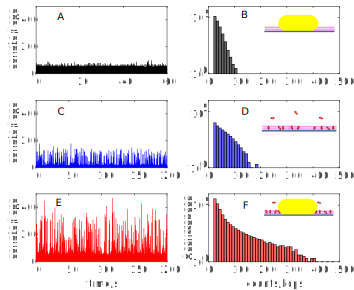
\includegraphics[]{timetrace_hist}
	\caption{Enhanced Fluorescence by a gold nanorod in a bilayer. Fluorescence time traces with binning time \SI{100}{\us}. 
	(A) Time trace of a gold nanorod in the absence of the dye, (C) Time trace with \SI{50}{\pM} ATTO 647N in the bilayer (E) Time trace with \SI{50}{\pM} ATTO 647N in the bilayer in presence of the gold nanorod. 
	The corresponding histograms of counts are shown to the right of each time trace (B, D, F).}
	\label{fig:timetrace_hist}
\end{figure}
The four-fold enhancement found above for a high-QY dye in the bilayer is much lower than the enhancements observed earlier for poorly emitting dyes.\cite{yuan2013thousandfold}
We ascribe this lower enhancement to reductions of both excitation and emission enhancements in our present case.
We first consider the position of the dye molecules with respect to the rod’s tips.
Because the dyes in the bilayer are confined in a \SI{5}{\nm} thick layer that is assumed to stick onto the glass substrate, they are largely outside the near-field hot spots at the tip of the \SI{50}{\nm} wide nanorod (see sketch in Fig.\ref{fig:schematic}), and are thus unable to explore the region of the hot spot with the highest intensity, resulting in a lower excitation enhancement than with 3D diffusion.
Indeed, we observed a much higher enhancement of ATTO 647N when the molecules were allowed to explore the whole space in 3D solution around the gold nanorod (see Supporting Fig.S\ref{SIfig:3D-enhc}; in this latter experiment, sucrose was added to the solution to match the diffusion constant with that in the bilayer).
Secondly, the emission enhancement is much reduced compared to low-quantum yield dyes.
Indeed, as the radiative channel of ATTO 647N (quantum yield \SI{65}{\percent}) is not competing with a strong nonradiative channel, the emission yield can at best be increased up to \SI{100}{\percent}, by a factor of only 1.5.\cite{khatua2014resonant}
\begin{figure}
	\centering
	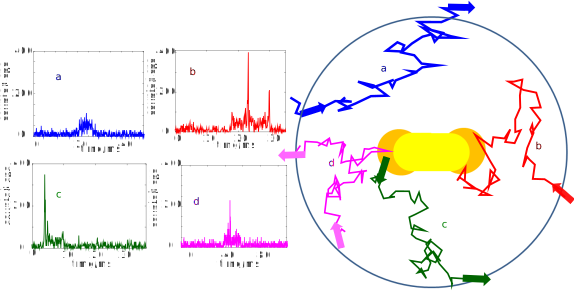
\includegraphics[width=0.9\textwidth]{enhnc_trajectories}
	\caption{Dye trajectories. (Left part) Different types of near-field enhanced intensity time traces observed in presence of the gold nanorod.
	(Right part) Schematic interpretation of the traces on the left, with molecules entering, leaving and diffusing in the far-field and near-field zone around an illuminated gold nanorod. 
	The colors of the schematic trajectories correspond to the colors of time traces.
	Blue: The molecule enters and leaves the far-field without passing through the near field; Red: the molecule enters the far-field area via the bilayer, crosses the near field twice and either bleaches or desorbs to the solution; Green: The molecule enters the near field from the solution and leaves via the far-field; Pink: the molecule enters the far field from the bilayer, crosses the near field, and finally leaves the far field again via the bilayer.}
	\label{fig:enhnc_trajectories}
\end{figure}
The time traces presented in Figure \ref{fig:timetrace_hist}A-E were furtheranalyzed to obtain lifetimes. 
Histograms of arrival times ofphotons are presented in Figure \ref{fig:lifetime_enhnc}.
The lifetimes were obtained taking the instrument response function into account.
The black time trace shows the photo luminescence of the rod in the absence of dye.
As the luminescence lifetime is very short, theassociated lifetime histogram (black) reproduces the instrumentresponse function.
For the pure dye in the absence of the rod, we find the usual bursts (Figure \ref{fig:timetrace_hist}C) as seen in standard FCS, and the associated decay is single exponential with a lifetime of \SI{3.7}{\ns} (blue).
The enhanced fluorescence time trace of rod with dye (red) gives rise to a nonexponential histogram, including ashort response from the rod luminescence and a secondcomponent which resembles the free dye decay.
Lastly, we applied a threshold of \SI{120}{kcps} to select enhanced bursts in the time trace of ATTO 647N in the presence of the rod.
The associated histogram (in green) is nonexponential.
This decay shows a strong lifetime reduction compared to the free dye.
\begin{figure}
	\centering
	\includegraphics[]{lifetime_enhnc}
	\caption{Fluorescence Decay. Normalized fluorescence decay of: ATTO 647N only (blue), ATTO 647N in presence of gold nanorod (red), events from intensity bursts with more than \SI{120}{kcps} (green), nanorod luminescence (black)}
	\label{fig:lifetime_enhnc}
\end{figure}
The decay of enhanced fluorescence is always faster than that of unenhanced fluorescence.
We attribute this shortened lifetime to a combination of both emission enhancement and fluorescence quenching.
Although we did not attempt to quantify the radiative and non-radiative effects on the dye, in the coming paragraph*s we can still use the lifetime and intensity to discriminate between enhanced photons and photons from the unenhanced background.

To perform fluorescence correlation spectroscopy (FCS), we prefer to increase the number of dye molecules in the confocal volume.
To this end, we incubated the bilayer with a solution of \SI{100}{\nM} ATTO 647N on the bilayer (See Fig. \ref{fig:schematic}C).
Because of the high background and the presence of dye aggregates from un-ruptured vesicles, the identification of gold nanorods is difficult.
As the lifetime of enhanced fluorescence and of nanorod luminescence is much shorter than that of ATTO 647N, we applied fluorescence lifetime imaging (FLIM) to distinguish the rods.
The lighter spots in the lifetime image (Fig.\ref{fig:schematic}D) indicate nanorods, which only rarely correspond to brighter spots in the fluorescence intensity image.

The fluorescence autocorrelation function is given by $G(\tau)=<I(t)I(t+\tau)>/<I(t)>^2$ and keeps track of the temporal fluctuations of the fluorescence intensity $I(t)$ (where $\tau$ is the lag time and ... represents time averaging).
For molecules confined to the bilayer, the correlation can be fitted with a two dimensional diffusion model in a Gaussian beam:
\begin{equation}
	G_{FF}(\tau)-1 = \frac{1}{N_{FF}}\bigg(1+\frac{\tau}{\tau_{FF}} \bigg)^{-1},
	\label{eq:2D-gauss-diffusion}
\end{equation}
where $N_{FF}$ represents the average number of molecules in the focal spot and $\tau_{FF}$ is the diffusion time in the focal spot.
The amplitude or contrast of the autocorrelation,$[G(0)-1]$ , directly gives the average number of fluorescent species in the detection volume, $N_{FF}=[G(0)-1]^{-1}$.
In presence of a nanorod, we fitted the FCS curves with the theoretical model of Langguth and Koenderink (see ref.\cite{langguth2014simple} and Supporting Information Sec.5).
In the model the molecule detection function is considered as the superposition of two coinciding 2D Gaussians, leading to the following correlation function:
\begin{equation}
	G(\tau)-1 = \frac{1}{<C>S_{MDF}^2}[\sum_{n}A_{nn}(\tau) + \sum_{n\neq m}A_{nm}(\tau)],
	\label{eqm:far-near-gauss}
\end{equation}
with n, m = F (far-field), or N (near-field),
\begin{equation}
	A_{n,m}(\tau)=S_nS_m\Bigg[\frac{2}{\pi\Big([\omega_n]^2 + [\omega_m^D(\tau)]^2 \Big)}\Bigg] ,
	\label{eqm:area-gauss}
\end{equation}
$\omega_m^D(\tau)=\sqrt{\omega_m^2 + *D\tau}$, $S_n=P_n\times A_n$ and $S_{MDF}^2=\Big[\sum_{n}S_n\Big]^2$,

where $P_n$ indicates the peak intensity and An the area of the Gaussian distribution.
The near-field width ($\omega_N$) and peak intensity ratio ($P_N=P_N/P_F$) were derived from the fitting. 
The contrast corresponding to $A_{NN}$ term (i.e near-field/ near-field correlation) at zero lag time can be given by:
\begin{equation}
	G_{NN}(0) = \frac{P^2\frac{\omega_N}{\omega_F}} {N_{FF}\Big(1+P\frac{\omega_N}{\omega_F}\Big)^2}.
	\label{eqm:contrast_enhnc}
\end{equation}
The autocorrelation of the time trace at \SI{100}{\nM} ATTO 647N is shown in Fig.\ref{fig:corr_enhnc}C.
The blue curve corresponds to the dye diffusing in the bilayer without gold nanorod.
The diffusion time in the far field $\tau_{FF}$ is related to the beam waist $\omega$ ($1/e^2$ radius of the detection area which was measured to be \SI{265}{\nm} of the beam and to the diffusion coefficient $D$ by $\omega^2=4D\tau_{FF}$.
For ATTO 647N in the bilayer, this time as determined from a fit of the autocorrelation is $3.95\pm0.05~ms$, which gives for the diffusion coefficient \SI{4.44}{\um\squared\per\s}.
From the value of $G_{FF}(0)$, the average number of dye molecules in the bilayer found to be 35 at \SI{100}{\nM} ATTO 647N in the confocal detection area of around \SI{0.22}{\um\squared}, i.e., \SI{160}{ molecules\per\um\squared}.
The same number of molecules in the diffraction-limited spot would correspond to a threedimensional concentration of \SI{0.8}{\uM}.
In the presence of gold nanorods, an extra component on a smaller time scale in the autocorrelation is observed.
From the red curve in Fig.\ref{fig:corr_enhnc}C, we obtained a near-field width of \SI[separate-uncertainty = true]{31(6)}{\nm}, around 10 times smaller than the far-field width.
The peak intensity ratio (P) between near-field and far-field was obtained to be $5\pm1.5$.
\begin{figure}[ht]
	\centering
	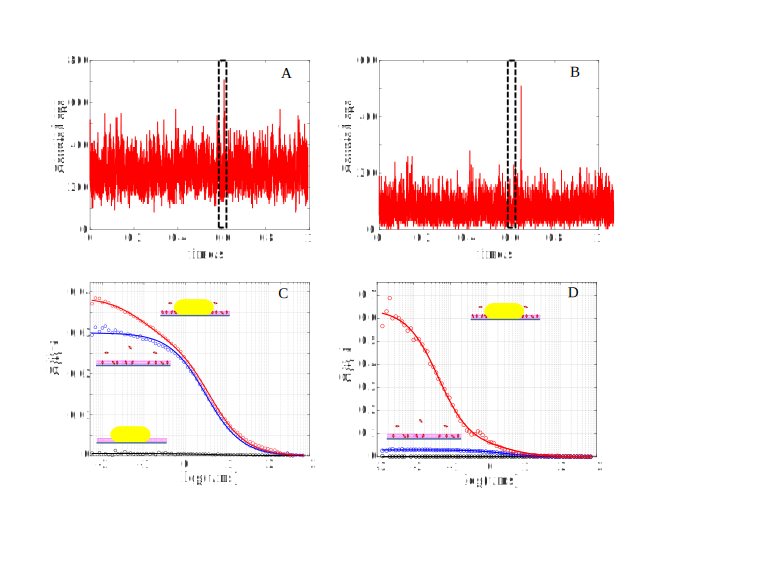
\includegraphics[width=0.8\textwidth]{corr_enhnc}
	\caption{Fluorescence correlation in high background. Fluorescence time trace of \SI{100}{\nM} ATTO 647N in the 
	presence of a nanorod before (A) and after (B) lifetime filtering. The dashed boxes highlight a near-field 
	burst in both traces. Autocorrelations of fluorescence intensity traces at \SI{100}{\nM} ATTO 647N before (C) and 
	after (D) lifetime filtering. Red circles: correlation in presence of the rod; blue circles: correlation in the 
	absence of the rod; black circles: correlation of the gold luminescence only (in absence of ATTO 647N).}
	\label{fig:corr_enhnc}
\end{figure}

The diffusion coefficient \SI{4.44}{\um\squared\per\s} obtained for ATTO 647N in the bilayer is close to the literature values of \SIrange{3}{4}{\um\squared\per\s}\cite{mach2010lipid} for other dyes and is similar to those of freely moving lipid molecules in the bilayer.
No correlation component was observed for the dyes in the solution because of the low fluorescence intensity and high background from the dyes diffusing in the bilayer.
In presence of a nanorod, we find the same long diffusion time again, corresponding to molecules diffusing in the diffraction-limited area, while we assign the shorter component to diffusion in the near-field of the gold nanorod, responsible for enhanced brightness of the molecules.
The near-field width is about 10 times smaller than the far-field diameter, and is consistent with near-field simulations and lifetime calculations around gold nanorods
of this size.\cite{khatua2014resonant,seelig2007nanoparticleinduced}
The near-field area is reduced by more than one order of magnitude (70 times in our case).
Assuming the diffusion coefficient to be same in the far field and near field, and applying the analysis for a Gaussian near-field intensity distribution, we obtain a diffusion 
time of \SI[separate-uncertainty = true]{57(11)}{\us} in the near-field from the relation $\omega^2=4D\tau_N$.
The peak ratio $5\pm1.5$ is close to the maximum enhancement factor of $4$ obtained from the burst analysis (vide supra) which confirms the results 
obtained in the FCS and shows that the maximum enhancement factor can simply be obtained from the FCS.
However, the contrast of the near-field correlation (0.01) is much weaker, which may make it difficult to distinguish this component in FCS experiments with lower signal-to-noise ratios.

As can be seen in Fig.\ref{fig:corr_enhnc}A, C, the contrast of the near-field component is weak, essentially because it is reduced by background.
To further enhance this correlation component, we can exploit a further difference between enhanced and unenhanced counts, namely their delay after excitation, less than \SI{2}{\ns} 
versus \SI{3.7}{\ns}, respectively.
We thus filtered out unenhanced photons by selecting photons detected within \SI{1}{\ns} from the excitation pulse, and computed their correlation function.
A typical time trace before and after filtering can be seen in Fig. \ref{fig:corr_enhnc} A, B.
The average background went down from $272~$kcps to \SI{74}{kcps}  and the signal-to-noise ratio of the enhanced signal improves accordingly, as can be seen for the burst marked in the box. 
The contrast of the near-field component in the filtered correlation has now been enhanced by about 60 times, making it easy to distinguish against the far-field correlation.
From the filtered correlation in Fig.\ref{fig:corr_enhnc}D, we find a near-field diffusion time of \SI[separate-uncertainty = true]{59(5)}{\us}, similar to the one deduced from the unfiltered correlation.
Shorter filtering windows lead to even shorter times for this near-field component, corresponding to larger emission enhancement and quenching at shorter distances.
However, this dependence is rather slow, so that the above number has physical meaning as the typical near-field diffusion time.
Of course, filtering down to very short times considerably reduces the signal-to-noise ratio (See Fig. S\ref{SIfig:cutoff-effect})
\begin{figure}[ht]
	\centering
	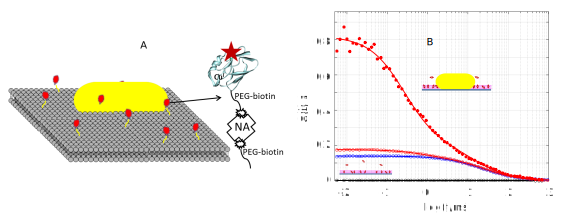
\includegraphics[width=0.8\textwidth]{Zn_azurin_efcs}
	\caption{(A) Scheme showing the labeling strategy for protein anchoring onto the bilayer.
	The Azurin labeled with ATTO 655 and biotin binds to DSPE-PEG-Biotin in the bilayer through Neutravidin.
	(B) Autocorrelation of the time traces of the labeled protein in absence of the nanorod (blue), in the presence of the nanorod (red circles) 
	and in the presence of the nanorod after lifetime filtering (solid red).
	Notice the higher correlation contrast after lifetime filtering in presence of nanorod.}
	\label{fig:Zn_azurin_efcs}
\end{figure}

The bilayer-nanorod platform can be used for biochemical applications.
We demonstrate this by anchoring a protein, azurin, onto the bilayer.
This protein with a copper metal center is known to mediate electron transfer in biological redox processes.\cite{kolczak2006azurin,Vijgenboom1997invivo}
To prevent electron transfer processes in the present experiments, we used azurin with a zinc metal center.
The protein's Lysine 122 residue was labeled with ATTO 655. 
As Zn-Azurin does not show electron transfer, electron transfer to or from the dye is excluded.
The anchored protein shows free mobility on the bilayer as can be inferred from the single decay component of the autocorrelation (Fig.\ref{fig:Zn_azurin_efcs}B, blue).
This component has a diffusion time of \SI[separate-uncertainty = true]{22(5)}{\ms} in the far field, which is around five times longer than the diffusion time of the free dye ATTO 647N.
We attribute this longer diffusion time to interactions and reduced mobility of the bulky anchoring among surrounding lipids. 
We now turn to the correlation curve in the presence of the nanorod.
The absence of any long-lived correlation component indicates that the protein continues to diffuse freely and does not stick to the solid surfaces. 
The near-field diffusion time for the protein was found to be \SI{318}{\us}, which is also around five times the near field time of ATTO 647N.
This confirms that diffusion is not significantly altered, even within \SI{30}{\nm} of the rod.

%===============================CONCLUSION==============================
\section{Conclusion}
A lipid bilayer substrate prevents the nonspecific sticking of dyes to a glass surface and thereby makes it possible to perform enhanced FCS around a metal structure with no hindrance in the diffusion kinetics.
The fluorescence of molecules in the near field always decays faster than that of far-field molecules.
The shorter lifetime of enhanced fluorescence can be used to discriminate the near-field signal from the high background in the far field.
The autocorrelation of the shorter lifetime component shows spectacular improvement in the correlation contrast which is helpful for studying FCS at high concentrations in presence of a strong background from unenhanced molecules.
The bilayer substrate with nanostructures can be used as a hybrid surface where probe molecules can either be functionalized to the surface or be kept free in the solution without any nonspecific interaction.
As lipid bilayers are close to biological membranes, many kinds of biochemical FCS experiments on the bilayer at physiological concentrations can be envisioned.
%===============================================================================================
%=================================SUPPORTING INFORMATION========================================
%===============================================================================================
\graphicspath{{chapters/c2_bilayer_efcs/si-figure/}}

\section{Supporting info}
\begin{figure}[ht]
  \centering
  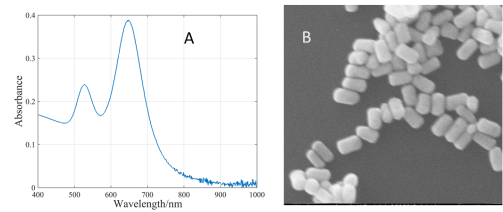
\includegraphics[width=0.8\textwidth]{AuNR_uv-vis_SEM}
  \makeatletter
  \renewcommand{\fnum@figure}{\figurename~S\thefigure}
  \makeatother
  \caption{\textbf{Gold nanorod characterization.} A, Extinction spectrum of a bulk gold nanorod suspension in water. B, Scanning electron microscope image of nanorods.
  The average dimensions of the nanorods are \SI[product-units=repeat]{90x50}{\nm}.}
  \label{SIfig: AuNR_uv-vis}
\end{figure}

\paragraph*{Chemicals}
Figure \ref{SIfig:chemical}A shows the chemical structure of the dye ATTO 647N used in the experiments.
The hydrophobic moiety of the molecule helps to enter the bilayer.
The lipid (Figure \ref{SIfig:chemical}B) has a zwitterionic head which helps to avoid nonspecific sticking.
\begin{figure}[ht]
  \centering
  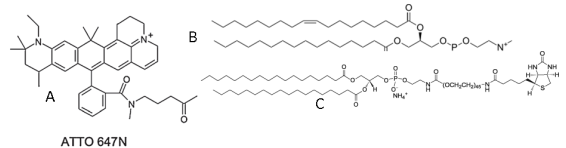
\includegraphics[width=0.8\textwidth]{chemical_picture}
  \makeatletter
  \renewcommand{\fnum@figure}{\figurename~S\thefigure}
  \makeatother{}
  \caption{Chemical structure of ATTO 647N (A), POPC lipid (B), DSPE-PEG(2000)Biotin (C)}
  \label{SIfig:chemical}
\end{figure}


\paragraph*{Bilayer Characterization}
Figure S\ref{SIfig:xz-scan} shows a raster-scanned image of a bilayer with \SI{100}{\nM} ATTO 647N in the XZ plane (perpendicular to the substrate). 
A higher intensity is observed at the glass-buffer interface showing the presence of dye in the bilayer.
The lifetime image helps to distinguish a nanorod (blue spot on the left of Fig. \ref{SIfig:xz-scan}B) against the background fluorescence.

\begin{figure}[ht]
  \centering
  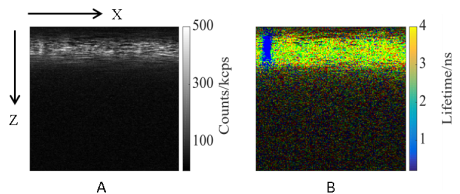
\includegraphics[width=0.8\textwidth]{xz_scan}
  \makeatletter
  \renewcommand{\fnum@figure}{\figurename~S\thefigure}
  \makeatother{}
  \caption{(A) Fluorescence intensity image (size \SI[product-units=repeat]{8x8}{\um}, and (B) fluorescence lifetime image (FLIM) both taken perpendicular to the plane of the lipid bilayer (from the glass surface at the top to the solution at the bottom).
  The bilayer was labeled by incubation with a solution of \SI{100}{\nM} ATTO 647N in Tris pH 9 buffer.}
  \label{SIfig:xz-scan}
\end{figure}

\begin{figure}[ht]
  \centering
  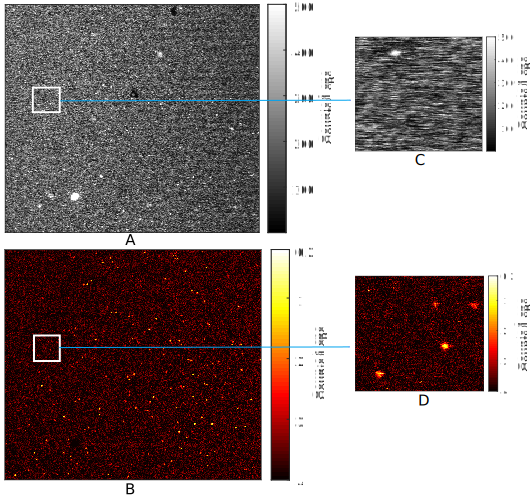
\includegraphics[width=0.8\textwidth]{xy_with_zoom}
  \makeatletter
  \renewcommand{\fnum@figure}{\figurename~S\thefigure}
  \makeatother{}
  \caption{ Intensity image (A) and lifetime image (B) of a \SI[product-units=repeat]{80x80}{\um} area of a glass substrate with spin-coated gold nanorods and covered with a supported lipid bilayer.
  The bilayer is labeled by incubation with \SI{100}{\nM} ATTO 647N.
  Intensity image (C) and lifetime image (D) of a zoomed-in area of the original image.}
  \label{SIfig:xy-scan}
\end{figure}


A large area of the bilayer labeled with ATTO 647N can be seen in Figure S\ref{SIfig:xy-scan}A.
The intensity is almost uniform across the whole area except for some bright and dark spots.
The bright spots are probably un-ruptured vesicles and the dark spots indicate holes in the bilayer.
Measurements described in the text have been conducted far away from these holes.
The bright spots in the lifetime image (Fig.S\ref{SIfig:xy-scan}C) indicate the nanorods.
Most of the bright spots in the intensity image do not correlate with the bright spots in the lifetime image.
This is the reason we rely on the lifetime image to locate the gold nanorods.


\paragraph*{Zooming in on intensity bursts}
\begin{figure}[ht]
  \centering
  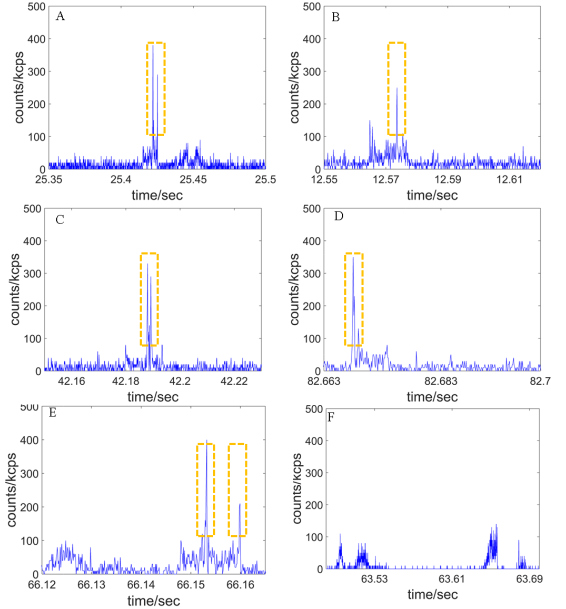
\includegraphics[width=0.8\textwidth]{zoomed_traces}
  \makeatletter
  \renewcommand{\fnum@figure}{\figurename~S\thefigure}
  \makeatother{}
  \caption{Zoomed-in time traces of the enhanced bursts (A-E) observed for ATTO 647N in the presence of a gold nanorod showing that the enhanced signal nearly always is embedded in the far field signal; (F) Time trace of ATTO 647N in the bilayer in the absence of gold nanorod.
  The full time traces were shown in Figure 1.}
  \label{SIfig:zoomed-trace}
\end{figure}


Figure S\ref{SIfig:zoomed-trace}A-E shows different enhanced bursts observed when ATTO 647N molecules diffuse around a gold nanorod.
The distinction is made on the basis of intensity.
Intensity levels above 100 kcps represent enhanced signals and have been marked by a dotted box.
In the bursts shown it can be seen that the near-field signal is observed only in the presence of the far-field signal.
A molecule travels some distance in the far field before it reaches the near field.
In absence of gold nanorod (Fig. S\ref{SIfig:zoomed-trace}F), we only see the far-field signal and no short bursts, as expected.


\paragraph*{Fitting of FCS curves}
As only probe molecules in the bilayer contribute to the signal, the FCS curves without nanorod were fitted with a two-dimensional Gaussian model:
\begin{equation}
  G_{FF}(\tau)-1 = \frac{1}{N_{FF}}\Bigg(1+\frac{\tau}{\tau_{FF}}\Bigg)
  \label{eq:2Dgauss}
\end{equation}
where $N_{FF}$ represents the average number of molecules in the focal spot and $\tau_{FF}$ is the diffusion time in the focal spot.
The amplitude of the autocorrelation, $G(0)-1$ directly gives the average number of fluorescent species in the detection volume, $N=[G(0)-1]^{-1}$.
At incubation with a solution of \SI{100}{\nM} ATTO 647N in buffer, the average number of molecules in the bilayer appeared to be 35.
Background corrections were negligible.


The gold nanorod enhances fluorescence and the enhanced signal in the near-field of the gold nanorod was observed only in the presence of the far field (diffraction limited area) signal.(Vide supra).
\begin{figure}%[ht]
  \centering
  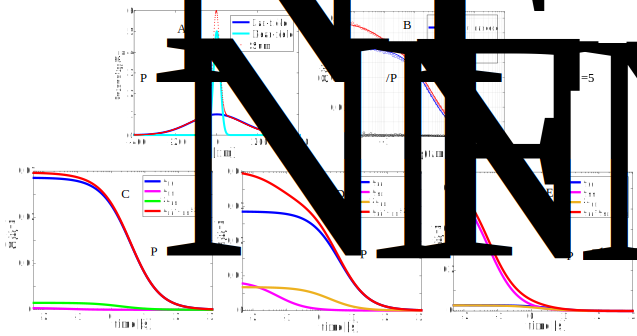
\includegraphics[width=\textwidth]{calc_enhc_corr}
  \makeatletter
  \renewcommand{\fnum@figure}{\figurename~S\thefigure}
  \makeatother{}
  \caption{\textbf{Simulation of high-background-enhancedFCS} (A) crosscut (red dots) through an intensity profile consisting of the sum of two Gaussians: far-field Gaussian (blue, waist=265 nm; peak height: $P_{FF}=1$) and near-field Gaussian (magenta, $waist=\SI{31}{\nm}$; peak height: $P_{NF}=5$).
  (B) Experimental autocorrelations of fluorescence intensity traces at \SI{100}{\nM} ATTO 647N in the presence of the rod (red circles), in the absence of the rod (blue circles), and of the gold luminescence only (black circles, in the absence of ATTO 647N).
  (C-E) Calculated autocorrelation for the entire intensity profile (red) and its constituents: the autocorrelation of far-field focus $A_{FF}$ (blue), the near-field $A_{NN}$ (magenta) and the 
  sum of identical cross-terms $2A_{FN}$ (green) with different peak heights $P_{N}/P_{F}=1$(C), $P_{N}/P_{F}=5$(D) and $P_{N}/P_{F}=90$(E).
  The calculated correlations fit best the experimental correlations for a peak height ratio of 5.
  This value is very close to the maximum factor of 4 enhancement obtained from direct comparison of burst intensities (main text).}
  \label{SIfig:calc_enhc_corr}
\end{figure}


The theoretical model of the correlation function was compared to experimental correlation functions.
In the model of Langguth and Koenderink\cite{langguth2016exact}, the molecule detection function is considered as the superposition of two coinciding 2D Gaussians.
We take a beam waist of \SI{265}{\nm} for the far field and \SI{31}{\nm} for the near-field.
The total correlations were calculated as:
\begin{equation}
  G(\tau)-1 = \frac{1}{<C>S_{MDF}^2}[\sum_{n}A_{nn}(\tau) + \sum_{n\neq m}A_{nm}(\tau)],
  \label{eq:far-near-gauss}
\end{equation}
with n, m = F (far-field), or N (near-field),
\begin{equation}
  A_{nm}(\tau)=S_nS_m\Bigg[\frac{2}{\pi\Big([\omega_n]^2 + [\omega_m^D(\tau)]^2 \Big)}\Bigg] ,
  \label{eq:area-gauss}
\end{equation}
$\omega_m^D(\tau)=\sqrt{\omega_m^2 + 2D\tau}$, $S_n=P_n\times A_n$ and $S_{MDF}^2=\Big[\sum_{n}S_n\Big]^2$,
where $P_n$ indicates the peak intensity and $A_n$ the area of the Gaussian distribution. 
Figure S\ref{SIfig:calc_enhc_corr}C-D shows calculated correlations for different peak intensity ratio ($P_F/P_N$). 
The red curve indicates the total correlation function and the other curves represent individual correlations (blue, green and magenta) that contribute to the total correlation.
Here we would like to emphasize that the contribution of the cross terms ($A_{FN}$) between far-field and near-field is not negligible, especially at low peak intensity ratios.

\newpage
\begin{figure}[ht]
  \centering
  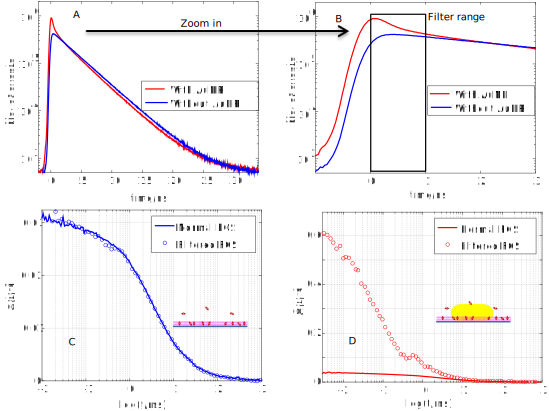
\includegraphics[width=0.8\textwidth]{lifetime_filtering}
  \makeatletter
  \renewcommand{\fnum@figure}{\figurename~S\thefigure}
  \makeatother{}
  \caption{\textbf{Lifetime filtering.} (A) Fluorescence decay of \SI{100}{\nM} of ATTO 647N in the presence (blue) and the absence (red) of a gold nanorod.
  (B) Zoomed-in part of the decay in Fig.S\ref{SIfig:lifetime-filtering}A at shorter time scales. 
  The dotted box indicates the range of arrival time of fluorescence counts considered for filtering the enhanced signal.
  The autocorrelation of normal and filtered time traces in the absence (C) and the presence (D) of nanorods. 
  Notice the invariance of the correlation in the absence of nanorods and the significant improvement in the correlation contrast in the presence of the nanorod.}
  \label{SIfig:lifetime-filtering}
\end{figure}

\paragraph*{Lifetime-based selection}
Correlation for shorter lifetime photons (enhanced signal) was obtained using only the photons arriving within 1 ns after the excitation pulse.
The blue decay in Figure S\ref{SIfig:lifetime-filtering}A represents the fluorescence decay of ATTO647N in the absence of gold nanorods and the red one in the presence of the gold nanorod. It can be clearly seen that the lifetime histogram in the presence of the nanorod exhibits a multicomponent decay.
All the photons falling in the dotted box in Figure S\ref{SIfig:lifetime-filtering}B were selected for correlation.
While the FCS curve in the absence of the nanorod remained unchanged as can be seen in Figure S\ref{SIfig:lifetime-filtering}C, the FCS contrast in the presence of gold nanorods showed a significant improvement.
This is because of the selective consideration of the enhanced signal in the near field and the suppression of background coming from the far field.

\begin{figure}[ht]
  \centering
  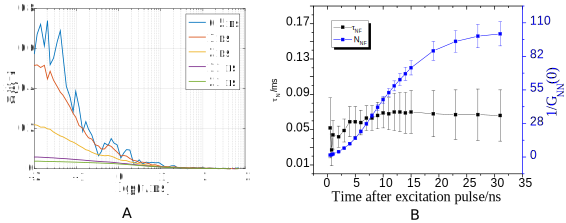
\includegraphics[width=0.9\textwidth]{cutoff_effect}
  \makeatletter
  \renewcommand{\fnum@figure}{\figurename~S\thefigure}
  \makeatother{}
  \caption{\textbf{Effect of cut-off range.} (A) Autocorrelation of time trace of ATTO 647N after lifetime filtering.
  The corresponding times after the excitation pulse are shown in the legend.
  Notice the significant increase in the noise between filtering times \SI{1}{\ns} (red) and \SI{0.5}{\ns} (blue).
  (B) Effect of the selection time window on the near-field correlation parameters.
  The near-field diffusion time is shown in black indicating minimal changes of time with selection range, whereas the number of molecules in the near field, shown in blue, undergoes a significant reduction.}
  \label{SIfig:cutoff-effect}
\end{figure}

\newpage
\paragraph*{Fluorescence enhancement in 3D diffusion}
Fluorescence enhancement experiments were performed with \SI{10}{\nM} ATTO 647N in \SI{70}{\percent} sucrose solution while the gold nanorods are immobilized on glass substrate.
We observed an average intensity of \SI{50}{kcps} for five molecules in the diffraction-limited volume in the absence of gold nanorods.
The intensity from a single molecule was 10 kcps.
In the presence of gold nanorods, bursts with a maximum of \SI{1200}{kcps} were observed corresponding with an enhancement factor of 110. (Figure S\ref{SIfig:3D-enhc})

\begin{figure}[ht]
  \centering
  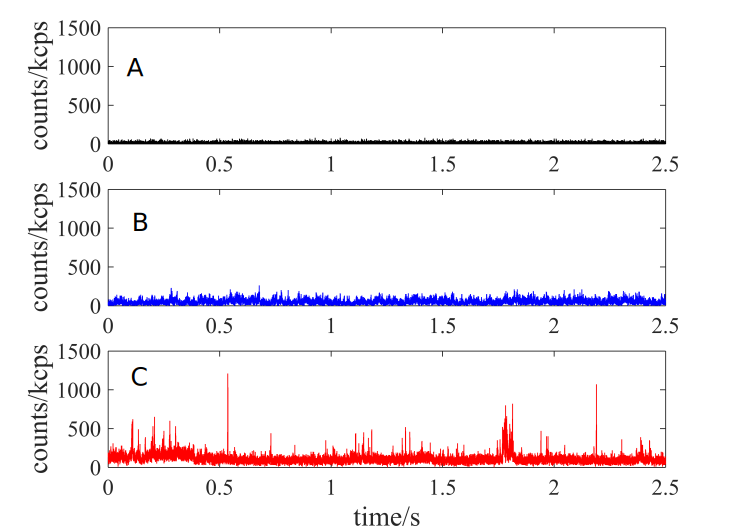
\includegraphics[width=0.8\textwidth]{3D_enhc}
  \makeatletter
  \renewcommand{\fnum@figure}{\figurename~S\thefigure}
  \makeatother{}
  \caption{\textbf{Enhancement in 3D.} Time traces with a binning time of \SI{100}{\us} of (A) Gold nanorod in sucrose with a constant intensity of \SI{20}{kcps}; (B) ATTO647N without gold nanorod in sucrose with average intensity of \SI{51}{kcps} for \SI{5}{ molecules} on average, as obtained from the autocorrelation function.
  This translates into a brightness of \SI{10}{ kcps\per molecule}; (C) ATTO 647N with gold nanorod in sucrose with a maximum intensity of \SI{1200}{ kcps}.
  Hence the fluorescence of ATTO 647N was enhanced by a factor of 110 by the gold nanorod.}
  \label{SIfig:3D-enhc}
\end{figure}


The enhancement factor of 110 is far bigger than the factor of 4 observed in the case of the lipid bilayer. 
The lifetime remained the same both in the bilayer and in the sucrose solution indicating no change in the quantum yield.
The difference in the enhancement factor can be explained by the accessibility of the hot spot for the diffusing molecules.
The nanorod used in the experiment is \SI{50}{\nm} thick.
In case of a bilayer, we suppose that the molecules are confined at the bottom to a layer of \SI{5}{\nm} thick.
Hence the diffusing molecules are not able to explore the most intense region of the hot spot, resulting in a weaker enhancement.
In the case of sucrose, however, the dye molecules diffuse through the whole space around the nanorod and occasionally reach the intense hot spot region resulting in a larger maximum fluorescence enhancements.
This observation supports the assumption that the bilayer does not cover the tips of the rod.

% \begin{figure}[ht]
%   \centering
%   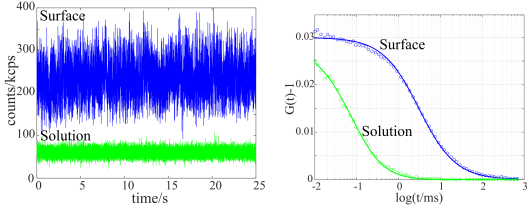
\includegraphics[width=0.8\textwidth]{surf_soln}
%   \makeatletter
%   \renewcommand{\fnum@figure}{\figurename~S\thefigure}
%   \makeatother{}
%   \caption{\textbf{Partitioning of the dye between surface and solution.} A) Time traces with a binning time of \SI{1}{\ms} of ATTO 647N on surface (blue) with an average intensity of \SI{235}{ kcps} and in solution (green) with an average intensity of \SI{60}{ kcps}.
%   (B) Autocorrelation of time traces of ATTO647N on surface (blue) and solution (green).
%   Notice the absence of correlation component corresponding to the solution in the blue curve.
%   The high background from the surface suppresses the correlation contrast of the dye in solution.
%   The similar magnitude of the autocorrelation contrasts indicates that the number of molecules on the surface is almost the same as the number of molecules in the three-dimensional detection volume in solution.
%   As the dye has a certain partition coefficient between the surface of the bilayer and the solution, the dye content on the surface can be controlled simply by changing the dye concentration in the solution.}
%   \label{SIfig:surf-soln}
% \end{figure}
% \references{chapters/c2_bilayer_efcs/efcs}
 \chapter{DNA transient binding on a gold nanorod}
\label{chapter:transient}
\graphicspath{{./chapters/c5_transient_binding/figures/}}

%============================== MAIN =======================================
\begin{abstract}
  Fluorescence enhancement by plasmonic nanostructures enables the detection of dyes with low quantum yield and improves the yield of quantum solid-state light sources.
  Here we demonstrate a DNA-based transient binding method to repeatedly and reproducibly study many single molecules by fluorescence enhancement on a single nanorod at the same spot on its tip.
  Heterogeneity of excitation and emission enhancements is avoided by looking at the same nanorod and the same binding site repeatedly.
  Bleaching of the plasmonic enhanced single molecules is no longer a problem as the bleached molecules are replaced by new ones.
  We characterize the distribution of enhancement factors and binding times. We investigate the fluctuations of the enhanced signal and the long-term stability of the binding sites.
\end{abstract}

\newpage
\section{Introduction}
Plasmonic nano-structures confine light to much smaller spatial dimensions than the optical diffraction limit. They enable detection of single molecules even at micromolar or millimolar concentrations, which is otherwise extremely challenging in conventional microscopy.\cite{levene2003zeromode,punj2013a,schuller2010plasmonics}
Optical nano-antennas strongly interact with quantum emitters, modifying their excitation and emission rates, and opening new non-radiative dissipation channels.
For emitters placed at the right position, plasmonic antennas can enhance their fluorescence by two to four orders of magnitude, enabling the detection of dyes with poor quantum yields.\cite{lakowicz2005radiative,anger2006enhancement,kinkhabwala2009large,acuna2012fluorescence,yuan2013thousandfold,khatua2014resonant}
The high electric field near the antenna leads to excitation enhancement while the high local density of optical states enhances the emission rates of the emitters, often leading to improvement in the brightness.
For emitters placed close to the metal surface, the nano-structure acts as an energy sink, quenching the fluorescence.\cite{seelig2007nanoparticleinduced,muskens2007strong,acuna2012distance,matsuzaki2017strong}
However, emission enhancement and quenching are highly dependent on the position of the dye with respect to the plasmonic structures. Therefore, fluorescence enhancement in the vicinity of nanoantennas is strongly inhomogeneous, because of the inhomogeneous electric field near the plasmonic structures, and because the position of the emitters cannot be controlled accurately. 


Different approaches to study single molecules by fluorescence enhancement involve free diffusion, non-specific sticking or immobilization of the emitters around the nanostructures. All of those approaches lead to random positioning of the emitters around the antenna.\cite{pradhan2016goldnanorodenhanced,yuan2013thousandfold,zhang2017gold}
This results in inhomogeneous excitation and emission of the fluorophores.
Uniform excitation and a better understanding of the photophysics of the fluorescent probes are necessary to fully understand the activity of biological or chemical systems as the light itself can perturb the system under study.
For instance, recently we found that the different excitation rates in the near field of a gold nanorod led to variations in midpoint potential of a redox indicator (methylene blue). The origin of this change was not clear as we could not precisely control the position of the dye.\cite{zhang2017gold}
The diffusion or immobilization methods also pose a limit to the observation time of the single molecules.
Diffusion times in the near field are often faster (\SIrange{1}{1000}{\us}) than the biomolecular processes (\SI{>1}{\ms}) making it difficult to study the slower process.
Whereas molecules can be immobilized almost indefinitely by chemical binding, bleaching limits their observation time. With immobilization by chemical binding, the number of single molecules that can be studied is thus limited to one per nano-antenna.


Here, we propose a transient binding method, by which fresh single dye molecules can be transiently immobilized on the same plasmonic hot spots. Nucleic acids, in particular DNA, offer highly predictable base pairing and binding energy, providing a simple and elegant mechanism for transient binding. Transient binding of short DNA strands has been applied in a super-resolution imaging technique called DNA-PAINT.\cite{jungmann2010singlemolecule,lin2012submicrometre,schnitzbauer2017superresolution}
The necessary blinking required for super resolution is generated by the transient binding of the short dye-labeled DNA ('imager') to its complementary target ('docking') strands on the structure in vitro or in vivo.
The chemistry and kinetics of single-strand DNA (ssDNA) binding are well understood at single-molecule level and widely available, thanks to the rapid development of DNA-PAINT and DNA-based biosensors.\cite{sassolas2008dna,jungmann2010singlemolecule}
The binding time of the imager strand to the docking strand can be tuned by the electrolyte concentration, the number of base pairs, the temperature, while the distance of the molecule to the antenna can be controlled by the number of base pairs, with a resolution of \SI{0.33}{\nm} per base pair.
Moreover, as DNA has a persistence length of \SI{\sim50}{\nm}, it acts as a rigid tether, thereby stabilizing the distance between the molecule and the plasmonic nanostructure.\cite{manning2006the}


In the current study, we chose gold nanorods as the plasmonic nanoantenna because of their simple structure, the high tunability of their surface plasmon resonance (SPR) and the accessibility of their near field to bigger molecules such as proteins and other biomolecules.
The nanorod can enhance the optical excitation intensity by two to three orders of magnitude when irradiated with a resonant laser.
The fluorescence enhancement relies on the overlap of the spectrum of the dye with the SPR of the rod and the laser excitation.
The optimum distance for enhancement is \SIrange{3}{5}{\nm}; closer to the rod, fluorescence quenching will dominate; too far away from the rod, the excitation enhancement will fade.\cite{khatua2014resonant}
With a linker of 10 base pairs, the distance of the dye to the surface is \SIrange{3.5}{4}{\nm}, provided the dye is at the further end of the imager strand.
By adjusting the concentration ratio of docking strands to passivating ligands, we can tune the average number of docking strands per rod, down to less than one per rod. The binding of the docking strand being a random process, the probability of having the docking strand on one of the tips of the rod will scale as the ratio of near-field area to total rod area.
In the present work, we wish to characterize the enhancement factors, the binding times, and the flexibility of the docking strand attached to the nanorod. Moreover, we show that a single gold nanorod with the right binding site is enough to study fluorescent enhancement with a statistically significant number of single molecules.


%====================EXPERIMENTAL SECTION=======================
\section{Methods}
\paragraph*{Materials.} Ethanol (\SI{99.8}{\percent}), methanol (\SI{99.8}{\percent}), 3-Mercaptopropyl) trimethoxysilane (MPTS, \SI{95}{\percent}), cysteamine (\SI{98}{\percent}), thioglycolic acid (\SI{99}{\percent}), Potassium chloride (\ce(KCl)), 4-(2-Hydroxyethyl) piperazine-1-ethanesulfonic acid (HEPES, \SI{99.5}{\percent}), Bovine serum albumin (BSA, \SI{96}{\percent}), Tris(2-carboxyethyl) phosphine hydrochloride (TCEP, \SI{98}{\percent}) were purchased from Sigma-Aldrich; 
Magnesium chloride (\ce{MgCl2}), Hydrogen peroxide (\ce{H2O2}, \SI{30}{\percent}), Sodium acetate (\ce{CH3COONa}, \SI{99}{\percent}), Potassium dihydrogenphosphate (\ce{KH2PO4}), disodium hydrogenphosphate (\ce{Na2HPO4}) from Merck;
Ammonium hydroxide (\ce{NH4OH}, \SI{30}{\percent}), Hydrochloric acid (\ce{HCl}, \SI{37}{\percent}) from Acros Organics;
succinimidyl 4-(p-maleimido- phenyl) butyrate (SMPB) from ThermoFisher.
Phosphate buffered saline (PBS) pH 7.4 contained \SI{137}{\mM} \ce{NaCl}, \SI{2.7}{\mM} \ce{KCl}, \SI{10}{\mM} \ce{Na2HPO4} and \SI{1.8}{\mM} \ce{KH2PO4}.
HEPES pH 7 buffer contain \SI{20}{\mM} HEPES. Acetate buffer pH 4 was prepared from \SI{164}{\mM} \ce{CH3COOH} and \SI{36}{\mM} \ce{CH3COONa}.


\paragraph*{Oligonucleotides.} The following DNA oligonucleotides were purchased from Integrated DNA Technologies:
\begin{itemize}
	\item DTPA-5'-ATA CAT CTA GAA ATT-3' (docking strand)
	\item -----3'-TAT GTA GAT C-Cy5-5' (imager strand)
\end{itemize}
Here DTPA represents a hexacyclic group with a dithiol that is used to strongly bind to gold, Cy5 denotes a red Cyanine dye, and A, T, C, G denote the DNA bases. Ten bases of docking strand are complementary to ten bases in the imager strand. The chemical structures and the binding scheme are shown in Figure S\ref{SIfig:AuNR-SS_bonding}.


\paragraph*{Silanization of glass surface.} Glass coverslips (Menzel-Glaser, \SI[product-units=repeat]{22x40}{\mm}, no. 1 thickness) were cleaned and activated for silanization before further functionalization.
The coverslips were sonicated in water (\SI{15}{\minute}) and ethanol (\SI{15}{\minute}). 
Then they were heated  at \SI{70}{\celsius} in a bath containing \ce{H2O}/\ce{NH4OH}/\ce{H2O2}(5:1:1) to remove organic impurities from the surface.
This step made the surface hydrophilic indicating the abundance of hydroxyl functionalities on the surface.
The cover slips were rinsed thoroughly in water and stored in ethanol for further use.
To activate the surface, the coverslips were flamed and treated for 30~min in a Teflon incubator with a \SI{1}{\percent} solution of (3-Mercaptopropyl)trimethoxysilane in methanol containing \SI{5}{\percent} glacial acetic acid.
Then the glass slides were rinsed and baked in an oven at \SI{65}{\celsius} for \SI{3}{\hour}.
This results in binding of the silane groups to the active hydroxyl groups and creates a thiol surface that can be used for conjugation with gold nanorods and for passivation of the substrate surface.


\paragraph*{Gold nanorod functionalization.} Gold nanorods (AuNRs) were synthesized using previously published seed-mediated growth in cetyl trimethyl ammonium bromide (CTAB). \cite{nikoobakht2003preparation}
The longitudinal surface plasmon of the AuNRs was \SI{640}{\nm} as obtained from the UV-vis spectrum, and their average dimensions were $\SI{90}{\nm}\times\SI{45}{\nm}$ as obtained from scanning electron microscopy images.
Excess of CTAB was removed by centrifugation and resuspension in milliQ water.
A thiolated coverslip was mounted in a homemade flow cell.
The AuNR solution was sonicated and immediately incubated in the flow cell for 10~min and then washed off with PBS buffer.
This resulted in around 10 isolated single gold nanorods per \SI{100}{\um\squared} area on the substrate.
A mixture of \SI{1}{\nM} thiolated docking strands and \SI{10}{\uM} methoxy-poly(ethylene glycol)-thiol (mPEG7-SH, MW 350) in pH 4 buffer was incubated overnight.
mPEG7-SH was used as the passivating ligand and allowed us to control the average number of docking strands on the nanorod.
The ratio between docking strands and passivating molecules was varied to get the desired number of docking strands at the tip of the nanorod.
The length and chemical nature of the passivating ligands were varied to test the flexibility of the docking strand.
Unless mentioned otherwise, the passivating ligand was mPEG.


\paragraph*{Surface passivation.} To prevent the unspecific sticking of imager strands to the surface, the rest of the glass surface was functionalized with bovine serum albumin (BSA).
This was achieved by incubating the coverslips with \SI{1}{mM} succinimidyl 4-(p-maleimidophenyl) butyrate (SMPB), \SI{20}{\uM} BSA and \SI{1}{mM} Tris(2-carboxyethyl)phosphine hydrochloride (TCEP) in HEPES pH 7 for \SI{1}{\hour}.
The succinimidyl group of SMPB binds to the BSA while its maleimide group binds to the thiol on the substrate. 
The unreacted chemicals were washed off with PBS pH 7 buffer.


\paragraph*{Imaging and time trace recording.} All the measurements were performed in a home-built confocal microscope that was equipped for Time Correlated Single Photon Counting (TCSPC).
Light from a pulsed picosecond diode laser (Power Technology, Little Rock, AR, USA) with a repetition rate of \SI{40}{\MHz} and a wavelength of \SI{635}{\nm} was passed through a narrow-band clean-up filter (Semrock LD01-640/8-25), then coupled into a single-mode optical fiber.
The output was collimated using a telescope system and reflected by a polychroic mirror (z488/633rpc) onto the back aperture of a high-numerical-aperture oil immersion objective (NA=1.4, Olympus UPLSApo 100x) and then focused to a diffraction-limited spot (\SI{300}{\nm}) on the surface of the coverslips.
An intensity of \SI[per-mode=repeated-symbol]{100}{\watt\per\cm\squared} was used to image the fluorescent objects on the surface.
Epi-fluorescence from the focal volume was collected through the same objective and focused on a pinhole for spatial filtering, and then passed through an emission filter (z488/635m "dual"-band emission filter, Chroma) to get rid of scattered laser light.
Finally, the fluorescence light was focused onto the active area of an avalanche photodiode (SPCM AQRH-15, Perkin Elmer Inc., USA).
The data was recorded by PicoHarp 300 (PicoQuant GmbH, Berlin, Germany) in time-tagged-time-resolved (t3r) mode which stores both arrival time and micro-time (time after laser excitation) of each photon.


Fluorescence images of the surface of the substrate were acquired by scanning a \SI[product-units=power]{10x10}{\um} area with a step size of \SI{50}{\nm} and a dwell time of \SI{1}{\ms}.
As the nanorods have very short photoluminescence lifetimes (shorter than the instrument response function IRF), they are easy to distinguish from the background of Cy-5 dye, with much longer fluorescence lifetime (see Figure S\ref{SIfig:trans_int_lt}).
The locations of the nanorods were saved and time traces were recorded for \SI{100}{\s} by parking the laser on the nanorods.
The laser intensity was \SI[per-mode=repeated-symbol]{10}{\watt\per\cm\squared}, 10 times smaller than the one used for imaging.
The nanorods with the desired number of transient-binding sites (inferred from the number of intensity levels) and fluorescence enhancement factor were selected for further measurements at different experimental conditions and durations.
%=======scheme========
\begin{figure}
	\centering
	\includegraphics[width=\linewidth]{scheme}
	\caption{\textbf{Transient binding schematic:}(left) Nanorods are immobilized on a thiolated glass surface and functionalized with docking strands and passivating ligands (mPEG7-SH).
	The coverslip surface is passivated with BSA to prevent non-specific sticking of imager strands to the glass.
	The imager-Cy5 strands in the solution  are shown with a gray dot on one end representing unenhanced fluorescence.
	One of the imager is bound to the docking strand at the tip of the nanorod and is shown with a bright red spot representing plasmon-enhanced fluorescence.
	(right) Reversible transient binding on the docking sites on a nanorod. The docking strand at the tip of the nanorod gives rise to enhancement while the one on the side of the rod exhibits no enhancement.}
  	\label{sch_trans:setup}
\end{figure}


\section{Results and discussion}
%========one vs many binding sites========
\paragraph{Number of binding sites.} The average number of docking strands on a gold nanorod is controlled simply by changing the concentration ratio between the docking DNA and mPEG7-SH.
Figure \ref{fig:timetrace1vsmany}(a) shows the time trace of transient binding on a gold nanorod with the ratio between docking and passivating strand maintained at 1:2000 and Figure \ref{fig:timetrace1vsmany}(c) at a ratio of 1:10000.
The concentration of imager strand was \SI{100}{\nM} with \SI{500}{\mM} \ce{NaCl} in PBS pH 7.4 buffer.
At ratio 1:2000, intensity bursts with different heights were observed and $5$ different peak heights can be distinguished from the intensity histogram with the maximum count rate at \SI{120}{ kcps} indicating an enhancement factor of $\sim60$ taking the count rate of un-enhanced imager as \SI{2} { kcps} (see Supporting Information, Fig S\ref{SIfig:timetrace_only_Cy5}).
The different peak heights are shown by the dashed lines and the numberings are done in increasing order of count rates.
The highest intensity shown by the arrow has two step-wise intensity changes resulting from two binding and unbinding events occurring during the same burst.
At ratio 1:10000, two intensity levels can be clearly distinguished both from the time trace and intensity histogram with the maximum enhancement factor of $\sim10$.
In all measurements, we adapted the laser power to the bursts to be detected, down to a factor of two in enhancement.
\begin{figure}[ht]
	\centering
	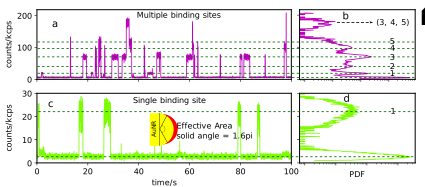
\includegraphics[width=\textwidth]{timetrace1vsmany}%width=\textwidth
	\caption{Time traces of transient binding of \SI{100}{\nM} imager with the docking sites on a gold nanorod with ratios between docking and passivating ligands of 1:2000 (a) and of 1:10000(c).
	The corresponding intensity histograms are shown on the right (b, d).
	The dashed lines connect the peaks in the histogram to the intensity levels in the time trace and the numberings are done in increasing order of the intensities.
	The arrow represents the combination of any two arbitrary levels from 1 to 5. 
	}
  	\label{fig:timetrace1vsmany}
\end{figure}


The gold nanorods were completely functionalized with mPEG7-SH and docking strands by overnight incubation.
Hinterwirth et al. showed that the coverage of \ce{PEG_7} on gold nanoparticles is \SI{4.29}{\per\nm\squared} and the packing density is mostly dependent on the steric hindrance rather than the chemical nature of the ligand.\cite{hinterwirth2013quantifying}
Therefore, a nanorod with dimensions \SI[product-units=repeat]{90x45}{\nm} should bind $5.5\times10^4$ chains, assuming similar reactivity of the passivating ligands and the docking strands.
At ratio 1:2000 between docking and mPEG7, out of ${\sim}27$ docking strands on the gold nanorod, ${\sim}5$ docking sites are observed through the fluorescence enhancement of imager strands by the gold nanorod.
Similarly, at 1:10000 ratio between docking and mPEG7 strands, ${\sim}1$ docking site is observed out of ${\sim}5$ docking strands on the nanorod.
The ratiometric study at two concentrations shows that \SI{20}{\percent} of the attached docking strands show fluorescence enhancement.
Assuming uniform distribution of the docking strands on the nanorod surface, the effective area on the nanorod for fluorescence enhancement can be calculated as \SI{20}{\percent} of its total area. We can thus estimate that the hot spots leading to a fluorescence enhancement larger than 2 times present an area of about \SI{1500}{\nm\squared} around each tip. This effective area will depend on the spectral overlap of the SPR of the rod with the dye spectra and laser, on the quantum yield of the dye, and on the distance of the dye to the surface of the rod.


One of the motivations for the present study is to observe the enhancement over and over again for the same binding site.
Figure S\ref{SIfig:bleaching_free_longtrace} shows transient binding on three different gold nanorods with different enhancement factors.
The two peaks in the intensity histogram of each rod and the absence of multi-step intensity bursts indicate that there is only one observable docking strand.
The narrow distribution of binding and unbinding times of imager strands on each particular nanorod over a time scale of \SI{1000}{\s} indicates that there is little variation in the DNA binding site over time.
However, the frequency of binding and unbinding varied from nanorod to nanorod, even for rods with a similar enhancement factor (Fig S\ref{SIfig:bleaching_free_longtrace}A, C).
This variation can be attributed to the different local environments in the PEG brush around each individual binding site, which can hinder the approach and binding of the imager strand to the docking strand.
For very long experiments (\SI{\sim1}{\hour}), we observed that the intensity bursts may completely disappear (Fig. S\ref{SIfig:dissociation_transbind}).
Deliberately applying high laser power also caused the transient binding to disappear, while some short bursts appeared.
Goodman et. al.\cite{goodman2016understanding} showed that Au-S bonds can break under some mW of pulsed laser irradiation or hundreds of mW of continuous wave (CW) laser illumination.
We attribute the short bursts appearing after irradiation with high power to non-specific sticking of imager strands to the rod. Indeed, not only the docking strands may have been released, but also some of the PEG passivating ligands, leaving comparatively free patches of bare gold surface.
While this light-induced dissociation can be useful for controlled release and delivery of drugs, it is detrimental to our transient binding experiments, where we wish to keep the docking strand permanently attached.
However, the dissociation of the docking strand from the gold can be delayed by using a CW laser instead of the pulsed laser employed in the current study.


%========Cysteamine vs peg========
\paragraph{Flexibility of the docking strand.} Different passivating ligands have been tested to understand their effect on the binding kinetics of imager and docking strands.
Two short linkers (less than \SI{1}{\nm} length), cysteamine with a basic head group (negative charge), and thioglycolic acid with a positive head group, were compared with the longer linker mPEG7-SH (\SI{\sim3.5}{\nm} length).
A transient-binding trace of a cysteamine-functionalized and of a PEG-functionalized nanorod can be seen in Figure \ref{fig:timetraceCysvsPeg}.
The intensity bursts for the cysteamine-functionalized nanorod are much noisier than the bursts of the PEG-functionalized nanorod.
We characterize the fluctuations of the fluorescence bursts by their autocorrelation function. We calculated the autocorrelation function for each of the intensity bursts. The averaged correlation functions of each time trace are shown in Figure \ref{fig:timetraceCysvsPeg}(C) for  PEG (green), cysteamine (magenta) and thioglycol (red) functionalization.
The autocorrelation of cysteamine and thioglycol-functionalization shows two exponential components while the autocorrelation for PEG shows a single exponential decay.
\begin{figure}[ht]
	\centering
	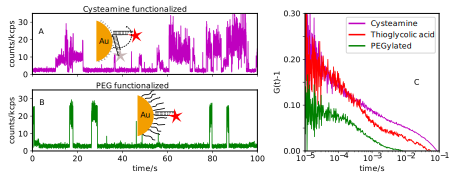
\includegraphics[width=\textwidth]{timetraceCysvsPeg}
	\caption{\textbf{Flexibility of the docking strand:} Time trace of transient binding on a gold nanorod with cysteamine (\ce{C2H7NS})(A) and mPEG7-SH (B) as passivating ligands.
	Notice the noisier intensity bursts in the case of cysteamine while the bursts for the PEGylated nanorod are much more stable.
	(C) Autocorrelation of intensity bursts for PEG (green), cysteamine (magenta) and thioglycol (red) functionalization.
	Autocorrelation values were obtained by averaging the individual autocorrelations from all bursts in each time trace. 
	Cysteamine and thioglycol have shorter chain lengths than PEG, and therefore allow more fluctuations of the distance between the nanorod and the imager dye (colored stars).}
  	\label{fig:timetraceCysvsPeg}
\end{figure}


The decay at shorter time scales (\SI{<1}{\ms}) present in all three cases is attributed to cis-trans conformational dynamics of Cy5.\cite{yeh2008tunable}
Cy5 can undergo cis-trans isomerization (Fig. S\ref{SIfig:AuNR-SS_bonding}). The trans form is planar and has stronger fluorescence, whereas the cis form has a distorted form with much lowered fluorescence.
The decay at longer time scales (\SI{\sim100}{\ms}) for cysteamine and thioglycol functionalization can be attributed to the interaction of the docking strand with the functionalized nanorod surface.
Although the movement happens at nanometer scales, it can be clearly observed because of the strong dependence of the enhancement on the position with respect to the tip of the nanorod.
As the docking strand wiggles, it can come close to the surface of the nanorod resulting in quenching or it can move away from the surface of the tip resulting in enhancement.
The persistence length of DNA\cite{manning2006the} is \SI{50}{\nm}, which suggests that the movement arises from the flexibility of the tether between the docking strand and the gold surface.
However, for PEG-functionalized nanorods, the slower fluctuations are missing. We attribute this to steric hindrance by PEG chains, which prevent interactions between the hybridized DNA and the gold surface. Although the PEG brush sterically hinders the DNA motion, the imager strands can still migrate into the brush and bind to the docking strand without compromising the transient binding.


%=======countrate vs duration==========
\paragraph{Binding time.}
The binding time of the imager to the docking strand depends on many factors: the number of base pairs involved in the binding, the salt concentration, the temperature.
For the current study, the number of base pairs involved in the binding was fixed to $10$ and all the measurements were performed at \SI{500}{\mM} \ce{NaCl} and at room temperature (\SI{298}{\kelvin}).
The length of the imager strand was chosen to be $10$ base pairs to get maximum fluorescence enhancement.
Khatua et al. obtained maximum fluorescence enhancement at a distance of \SIrange{3}{5}{\nm} from the tip of the gold nanorod for the low-quantum-yield dye Crystal Violet.\cite{khatua2014resonant}
Combining the length of DNA with that of the linkers between gold and DNA and between DNA and dye, we obtain a distance of \SI{\sim4}{\nm}, which should result in optimum enhancement.
The binding times of the imager observed from the time traces are plotted against the intensity of the bursts in the scatter plot of Figure \ref{fig:countrate_vs_duration}(A).
For low count rates we find more points with long dwell times, while at higher count rates, most of the bursts have short dwell times. 
The average burst duration clearly declines for count rates larger than \SI{\sim25}{kcps}.
We assign the reduction of burst duration for high count rates to bleaching of the dye. For low enough count rates, the burst duration will be limited by the binding time of the imager strand, rather than by the bleaching of the dye. We thus attribute the burst duration at low count rates (below \SI{\sim25}{kcps}) to the binding time of the imager.
Above \SI{\sim25}{kcps}, the dye bleaches before the imager strand unbinds from the docking strand, resulting in a shortened burst duration. We thus selected a maximum threshold of \SI{\sim25}{kcps} for estimating the binding kinetics. The histogram of binding times of intensity bursts with count rate less than \SI{\sim25}{kcps} is shown in Figure \ref{fig:countrate_vs_duration}(B), which appears to decay exponentially with a characteristic time of \SI{1.13}{\s}. The binding time of \SI{1.13}{\s} for 10-base-pair-binding at \SI{500}{\mM} \ce{NaCl} is similar to the value of \SI{5}{\s} obtained previously.\cite{jungmann2010singlemolecule}

\begin{figure}[ht]
	\centering
	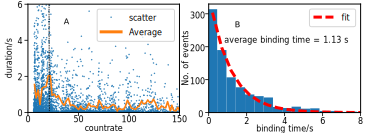
\includegraphics[width=\textwidth]{countrate_vs_duration_nophtns}
	\caption{\textbf{Binding time:} (A) Scatter plot of the burst duration versus count rate for intensity bursts in transient binding events. The data were obtained from $24$ nanorods with 1 to 5 docking sites on each of them. The vertical line indicates the count rate above which bleaching starts to govern burst duration.
	(B) Histogram of binding times of intensity bursts with count rates smaller than \SI{25}{ kcps}. The threshold was selected to exclude most bleaching events. From the exponential fit, we find an characteristic binding time of \SI{1.13}{\s}.}
  	\label{fig:countrate_vs_duration}
\end{figure}


%========Enhancement statistics=========
\paragraph{Enhancement distribution.}
Considering the strongly inhomogeneous near field of the nanoantenna, we expect a wide distribution of enhancement factors.
Figure \ref{fig:int_lt_distribution}(A) shows the distribution of burst intensities obtained for $24$ nanorods with 1 to 5 observable binding sites. The average count rate of all those bursts was \SI{53}{kcps}, corresponding to an average fluorescence enhancement factor of $\sim25$.
The possible positions of the dye at the tip of nanorod, assuming the tether to stand perpendicular to the surface, are shown in Figure \ref{fig:int_lt_distribution}.
The color map shows the optical intensity simulated by finite difference time domain (FDTD) in COMSOL. The lifetime histogram of enhanced fluorescence is shown in magenta (Figure \ref{fig:int_lt_distribution}(C)) while that of unenhanced fluorescence (in absence of intensity bursts) is shown in green.
The lifetime of unenhanced Cy5 is \SI{1.8}{\ns} while the lifetime histogram of enhanced bursts cannot be distinguished from the instrument response function.
\begin{figure}[ht]
	\centering
	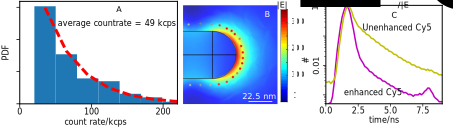
\includegraphics[width=\textwidth]{lifetime_scatplot}
	\caption{Enhancement statistics.(A) Histogram of count rates of intensity bursts of transient binding obtained from $24$ gold nanorods with 1 to 5 docking sites on each of them.
	The average count rate was \SI{53}{ kcps} with an enhancement factor of $\sim 25$.
	(B) Optical intensity map of the nanorod. The red stars indicate the positions the dye can occupy at the surface of the nanorod.
	The color bar is the normalized intensity.
	Both the enhancement factor and the number of possible binding sites are functions of the distance of the dye to the tip. The strongest enhancement corresponds to a small disk at the rod's tip, whereas the large areas on the rod sides correspond to much lower enhancements.
	(C) Lifetime histogram of all the intensity bursts found in the time trace of Figure \ref{fig:timetrace1vsmany}(a) shown in magenta. The lifetime histogram of the unenhanced fluorescence is shown in green.
	}
  	\label{fig:int_lt_distribution}
\end{figure}


As the docking strands are functionalized randomly on the nanorod without specificity to the tip, we expect to find enhancement factors corresponding to all possible positions of the dye at a fixed distance ( 4 nm) from the gold surface.
The maximum enhancement factor observed is 100, which is reasonable for a dye with a high quantum yield (\SI{30}{\percent}) and for an excitation enhancement of \SI{\sim300}{times} by the gold nanorod.
A previous study of the dye crystal violet showed an excitation enhancement of about hundred times. Because this dye has low quantum yield (\SI{1}{\percent}), a fluorescence enhancement of thousand-fold resulted from excitation enhancement and a 10-fold radiative enhancement. The radiative enhancement strongly depends on the quantum yield of the dye. Poorer quantum yields give rise to larger radiative enhancements. For Cy5 with a higher quantum yield, no significant radiative enhancement is expected, and the fluorescence enhancement is expected to stem mainly from excitation enhancement.
The most intense bursts come from close to the center of the tip while weak bursts originate from the sides.
The histogram of burst heights should thus be related to the distribution of light intensity at a distance of about \SI{4}{\nm} from the surface of the nanorod.


The lifetime histogram of enhanced fluorescence cannot be distinguished from the instrument response function. Therefore, the fluorescence rate (combining radiative and non-radiative rates) is enhanced by at least a factor of 10 (the lifetime of Cy5 away from the nanorod is \SI{1.8}{\ns}). However, with our current data, we cannot distinguish radiative from non-radiative contributions.
The previous study\cite{seelig2007nanoparticleinduced} shows that even at a distance of \SI{15}{\nm}, the lifetime is already reduced by a factor of 10.
As in the current study, the distance of the dye is just \SI{4}{\nm}, we expect a much shorter lifetime which requires a high-resolution TCSPC to be measurable.
% XXXrewrite this in a more neutral wayXXX As we don't expect much enhancement in the quantum yield of Cy5, quenching is probably a main contribution to the shortening of the lifetime.


\section{Conclusion}
We demonstrated the observation of many single molecules with equal enhancement factors on a single gold nanorod with a single binding site.
Different nanorods showed different enhancement factors because they presented different positions of the docking strand, in addition to different plasmon resonances.
Once a nanorod is identified with the desired enhancement factor, many single molecules can be studied with the same excitation and emission yields.
The effort to find the best enhancement factor can be reduced by specifically attaching the docking strand at the tip of the rod.
This transient binding method can be applied to different kinds of plasmonic nanostructures, where the position of the emitter can be controlled by proper DNA engineering.
Similarly, different biomolecules and quantum emitters can be studied by attaching them to the imager strand.

%=========================== SUPPORTING INFORMATION ==========================
\graphicspath{{chapters/c5_transient_binding/si-figures/}}
%============================ MAIN ==========================
\section{Supporting info}
\begin{figure}[ht]
  \centering
  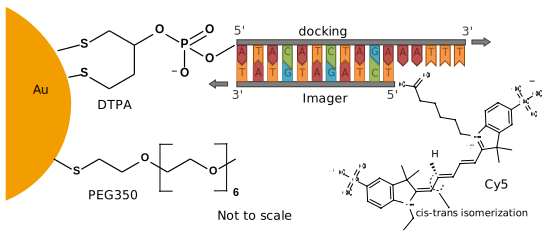
\includegraphics[width=0.8\textwidth]{AuNR-SS_bonding}
  \makeatletter
  \renewcommand{\fnum@figure}{\figurename~S\thefigure}
  \makeatother
  \caption{\textbf{Binding to gold surface} The chemical structures of different components in the transient binding scheme.
  The docking strand is attached to the nanorod through DTPA, which has two thiols attached to the gold atoms.
  The sequence of the docking and the imager strand are shown with their complementary binding.
  The imager strand is labeled with Cy5 at its 5' end.
  The rest of the nanorod surface is functionalized with PEG350, which has 9 monomers giving it a length of \SI{\sim3}{\nm}.}
  \label{SIfig:AuNR-SS_bonding}
\end{figure}

\begin{figure}[ht]
  \centering
  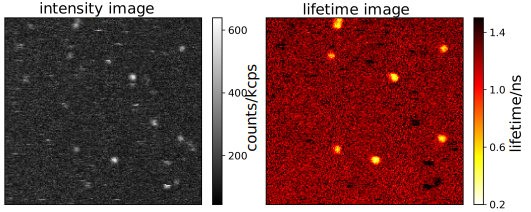
\includegraphics[width=0.8\textwidth]{trans_int_lt_img}
  \makeatletter
  \renewcommand{\fnum@figure}{\figurename~S\thefigure}
  \makeatother
  \caption{A \SI[product-units=power]{10x10}{\um} scanning image of the surface of the substrate with gold nanorod functionalized with docking strand and mPEG7-SH.
  The solution contains \SI{100}{\nM} imager strand in PBS pH 7.4 buffer with \SI{500}{\mM} \ce{NaCl}.
  The image on the left shows counts per millisecond while the image on the right shows the lifetime.
  The spots on the lifetime image correspond to the gold nanorods as they have a much shorter lifetime than the instrument response function.}
  \label{SIfig:trans_int_lt}
\end{figure}
% \subsection*{Replenish and recyacle}
\begin{figure}[ht]
  \centering
  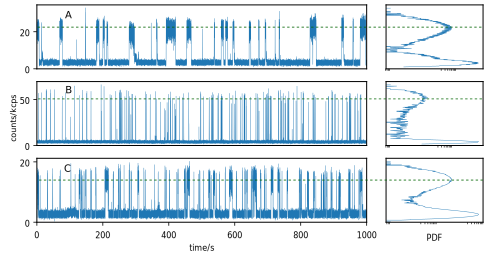
\includegraphics[width=\textwidth]{bleaching_free_longtrace}
  \makeatletter
  \renewcommand{\fnum@figure}{\figurename~S\thefigure}
  \makeatother
  \caption{\textbf{Many single molecules bind to the same binding spot on the same nanorod.} Time traces of three different nanorods, each of them with a single binding site, but with different enhancement factors.
  The histogram of intensities for each time trace is shown on the right and the two peaks indicate the presence of only one observable docking strand.
  Notice the different binding kinetics of trace A and trace C although they have similar enhancement factors.}
  \label{SIfig:bleaching_free_longtrace}
\end{figure}

\begin{figure}[ht]
  \centering
  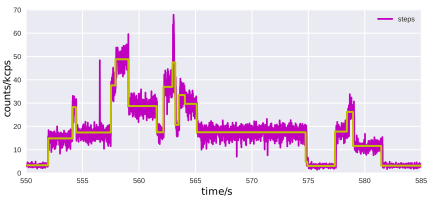
\includegraphics[width=\textwidth]{step_timetrace}
  \makeatletter
  \renewcommand{\fnum@figure}{\figurename~S\thefigure}
  \makeatother
  \caption{\textbf{Multi-step transient binding:}Time trace on a functionalized gold nanorod with multiple transient binding events appearing on top of each other.
  The association and dissociation of each imager strand can be distinguished from the step height and the time of appearance. }
  \label{SIfig: step_transbind}
\end{figure}

% \subsection*{Transient binding on substrate}
\begin{figure}[ht]
  \centering
  \includegraphics[width=\textwidth]{timetrace_only_Cy5}
  \makeatletter
  \renewcommand{\fnum@figure}{\figurename~S\thefigure}
  \makeatother
  \caption{\textbf{Transient binding without nanorod:} (A) Schematic of the transient binding.
  The docking strand was immobilized on the surface through neutravidin and biotin bonding.
  The solution contained \SI{100}{\nM} imager-Cy5 in PBS pH 7.4 buffer.
  Scanning image  in the absense (B) and presence (C) of docking strand on the surface showing the specificity of binding of the imager to the docking strand.
  (D) Time trace of transient binding on a single neutravidin-docking site at \SI{\sim 0.1}{\kW\per\cm\squared} power density, 10 times higher than the laser power used for measurement on the nanorod. The burst heights are \SI{\sim 20}{ kcps} corresponding to single imager-Cy5.
  To compare with the bursts from nanorods and calculate the enhancement factor, the count rate can be divided by 10 to match the laser power on the nanorod as the intensity varies linearly at such low powers.
  A count rate of \SI{2}{ kcps} for unenhanced Cy5 has been used in the main text. 
  }
  \label{SIfig:timetrace_only_Cy5}
\end{figure}
% \subsection*{Dissociation of docking strand}
\begin{figure}[ht]
  \centering
  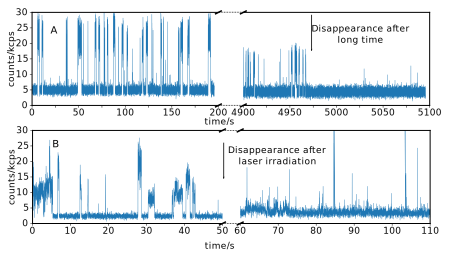
\includegraphics[width=\textwidth]{dissociation_transbind}
  \makeatletter
  \renewcommand{\fnum@figure}{\figurename~S\thefigure}
  \makeatother
  \caption{\textbf{Dissociation of docking strand.}
  (A) The time trace on the top is recorded on a gold nanorod until no docking events any more are observed.
  The transient binding events never reappeared, even after re-flushing with imager strand and realigning the laser focus.
  (B) The transient binding trace on a gold nanrod before and after irradiation with high laser power (\SI[per-mode=repeated-symbol]{1000}{\watt\per\cm\squared}, \SI{40}{\MHz}).
  }
  \label{SIfig:dissociation_transbind}
\end{figure}
% \references{chapters/c5_transient_binding/transient_binding}
\chapter{Binned and binfree analysis of Fluorescence Enhancement by gold nanorod on a 2D layer}
\section{Introduction}
\section{Experimental Method}
\section{Simulation method}
\section{Results and Discussion}
\section{Conclusion}
\chapter{Dynamic heterogeneity in single electron-transfer proteins}
\label{chapter:azurin}
\graphicspath{{./chapters/c4_azurin_sm/main/}}
%============================== MAIN =======================================
\begin{abstract}
	Conformational dynamics of proteins plays a crucial role in their biological activity. Single-molecule studies have revealed the spread of reaction rates of enzymes, which was not accessible in ensemble measurements.
	The energy landscape of an enzymatic reactions consists a large number of substates with a rugged energy landscape.
	However, the heterogeneous nature of dynamics obtained from the analysis of single-molecule traces and their generality is still hotly debated.
	Here we provide evidence of conformational heterogeneity in the complex formation of an electron-transfer protein, azurin, with redox-active partners.
	We characterize the electron-transfer dynamics of single azurin molecules from time traces, histograms of bright and dark times, and correlation functions of redox events. 
\end{abstract}
\newpage
%============================ Introduction =====================================
\section{Introduction}
Enzymes perform metabolic processes inside the cell with minimal energy requirements.
Conformational fluctuation of enzymes has got attention since the finding of non-exponential distribution of kinetic rates for an ensemble of myoglobin. \cite{frauenfelder1991the,ansari1985protein,stein1985a,henzler-wildman2007dynamic}
Conformational substates might hold the answer to the evolution of highly complex enzymes to perform efficient conversion of substrate to product.
Single-molecule spectroscopy has revealed the dynamic fluctuation of enzymes covering many orders of magnitude.\cite{lu1998single-molecule,yang2003protein,english2006ever-fluctuating}
However, the evidences of heterogeneity from the analysis of single-molecule time traces has been strongly debated.
Blank and coworkers have shown that the non-exponential distribution in the turn-overs of enzymes might be an artifact of the analysis of the time traces.\cite{terentyeva2012dynamic}
They showed that both threshold and change point analysis, to find transitions on a intensity time trace, lead to non-exponentiality in the distribution of turn-over times.


Dynamics of electron transfer in metalloproteins are also of high interest.\cite{marcus1985electron,dooley1981spectroscopic}
Efficient electron transfer in living cells is essential for energy metabolism and storage.
Metallo proteins are promising candidates for bio-electronic devices and efficient energy conversion as a biofuel.
Copper proteins along with iron proteins play a crucial role in the biological redox reactions. \cite{solomon2004electronic,solomon2001oxygen,peisach1974structural,canters1993engineering} 
Similar to enzyme-substrate complex formation, electron transfer occurs through the formation of a complex between a metallo(redox) protein and its redox partners.


Electron-transfer proteins are characterized by their electron-transfer rates and midpoint potentials.
Subtle changes in the structure of proteins may lead to variations in the electron-transfer rates.
Do redox proteins posses conformational substates in a particular oxidation state?
To look for heterogeneity, We will investigate electron-transfer rates of the redox protein azurin across many single molecules and of single azurins as a function of time.


Azurin is a copper protein  with molecular weight of \SI{\sim14}{\kilo\dalton}, which is believed to be taking part in redox homeostasis in cells.
A copper metal center is found in the so-called northern region of the protein matrix.
The surrounding ligands of the copper ion result in a $\pi-\pi*$ transition giving the protein a blue color (absorption in \SIrange{590}{620}{\nm}) in the Cu(II) state.
Cu(I)azurin is colorless due to the absence of the absorption band in the red.
The oxidation state of single azurin molecules can be determined by attaching a fluorophore whose emission overlaps with the absorption of Cu(II)azurin.\cite{kuznetsova2006a,kuznetsova2008the}
The fluorescence of the label strongly depends on the oxidation state of the copper.
In the Cu(II) state, the fluorescence is quenched while in the Cu(I) state the fluorescence is reserved.
The durations of high intensity bursts are denoted as bright times and the durations of low intensity bursts are denoted as dark times.


We study electron transfer in labeled single azurins while they react with electron mediators.
The redox potential of the solution is varied by applying an electric potential to a fixed concentration of electron mediators.
The distribution of electron-transfer rates across many single azurins was compared with the distribution of electron-transfer rate of a single azurin as a function of time.
The dynamics of single azurins was characterized by their intensity time traces, intensity correlations, histograms of bright and dark times, and the correlation of bright and dark times.

% \begin{itemize}
% 	\item Dynamic properties of enzymes have been focus of much research: Frauenfelder, Eaton, Onuchic, Kern. Single molecule: Xie HP Lu, H. Yang, van Oijen, Hofkens, Blank, Goldsmith
% 	\item Also the dynamic properties of ET proteins are of high interest: Marcus, Canters, Eaton
% 	\item Characteristic of ET-redox proteins are E0 and ET kinetics.
% 	\item Question: are these properties distributed in an ensemble and if so in what sense. Ergodicity, time and ensemble averages: Barkai
% 	\item We have investigated this by studying the E0 and the k's by SM techniques
% 	\item Do this by applying electric potential and looking at life times of reduced and oxidized state.
% 	\item Can do this by fluorescent labeling because the fluorescence is strongly dependent on the oxidation state through FRET.
% 	\item We will show that $...$
% \end{itemize}
%%%%%%%%%%%%%%---------- EXPERIMENTAL SECTION ----------%%%%%%%%%%%%%%%%%%%%
\section{Experimental section}

\paragraph*{Protein synthesis.}
Azurin (wild type) from \textit{Pseudomonas aeruginosa} was expressed in \textit{E. Coli} and purified as described before \citep{kamp1990purification}.
BL21 \textit{E.coli} cells were transformed with the PGK22 plasmid that carries the gene for azurin.
The cells were cultured in Luria Bertani (LB) medium.
Then the cells were harvested and resuspended in a \SI{20}{\percent} (w/v) sucrose solution in Tris pH 8 buffer containing \SI{1}{\mM} EDTA.
The solution was centrifuged (\SI{8000}{ rpm}, \SI{20}{\minute}) and the supernatant was collected.
Copper sulfate was added to the solution for insertion of Cu into the active site of azurin.
The unwanted proteins were precipitated by addition of concentrated acetic acid until pH 4. 
The turbid solution was centrifuged at \SI{8000}{ rpm} for \SI{20}{\minute}.
The supernatant was loaded on a CM Sepharose fast flow column and elution was performed in an Akta purifier (GE Healthcare) with a pH gradient from 4 to 6.9 in 
\SI{50}{\mM} ammonium acetate.
Fractions containing azurin (inferred from the absorbance at \SI{290}{\nm} and \SI{620}{\nm}) were collected and reduced with sodium dithionite.
At this stage the solution contained both zinc and copper azurin.
The azurins were purified in a DEAE sepharose column by a salt gradient of 0 to \SI{50}{\mM} NaCl in Tris pH8 buffer. 
Fractions containing copper azurin and zinc azurin were collected and concentrated separately.
The purity of the samples was checked by gel electrophoresis (PAGE, on polyacrylamide gel with sodium dodecyl sulphate, SDS) and by UV/Vis spectroscopy (Cary 50 spectrophotometer, Varian Inc., Agilent Technologies, USA).
The azurin was further appeared on SDS gel PAGE at $\sim$\SI{14}{ kDa}.
Both zinc and copper azurin showed a characteristic shoulder at ${\sim}$\SI{290}{\nm} while Cu azurin showed an additional 
broad absorption peak at \SI{620}{\nm} when oxidized, as can be seen in Figure-S\ref{SIfig: switching}. 
The ratio $OD_{\SI{628}{\nm}}/OD_{\SI{280}{\nm}}$ for Cu azurin was 0.56, which indicated a purity of more than \SI{95}{\percent}. 
The concentrated protein was stored at \SI{-80}{\celsius} until further use.


\paragraph*{Fluorescent labeling.}
The labeling protocol was based on previous work \cite{nicolardi2012topdown}.
ATTO655 NHS-ester was bought from ATTO-TEC GmbH and used without further purification.
The azurin solution was equilibrated with HEPES pH 8.3 for a higher efficiency of the amine-NHS-ester reaction.
ATTO655 was chosen to label the protein because of its photostability and inertness (unreactive) to the redox chemicals used in the study.
A mixture of \SI{200}{\uM} azurin and ATTO 655 NHS-ester (1:1) was incubated for \SI{45}{\minute}.
The NHS-ester group reacts with one of the amine groups on the protein.
The unreacted dyes were removed with a HiTrap desalting column.
The labeled protein was concentrated in Tris pH 8.5 buffer by centrifuging in a \SI{3}{ kDa} Amicon ultra-filter.
The labeled protein was further purified by ion exchange chromatography in a \SI{1}{\mL} MonoQ column (GE Health).
The different peaks obtained (see Figure S\ref{SIfig: peak_sep}) correspond to different numbers and positions of the dye on the azurin surface. 
Peak III corresponds to proteins labeled at Lysine122 position \cite{nicolardi2012topdown}.
For this position of the dye, the protein construct shows a high fluorescence switching ratio \SI{90}{\percent} between oxidized and reduced conditions as can be seen in Figure S\ref{SIfig: peak_sep}. This fraction was chosen for our single-molecule experiment as the two states can be distinguished easily.
The same protocol was used for Zn-azurin labeling and similar peak separations were observed.
The fluorescently labeled proteins were then reacted with biotin-PEG-NHS (MW 3400) in phosphate-buffered saline (PBS) pH 7.4 buffer with a ratio 1:5 (azurin : biotin-peg-NHS) to make sure each protein has at least one biotin.
The free biotin was then removed by centrifuging in a \SI{3}{ kDa} Amicon ultra-filter.
The biotin on the protein will be used for immobilization on the glass surface.


\paragraph*{Functionalization of coverslips.}
The functionalization of the glass surface was achieved according to previous work with slight modifications.\cite{gupta2012involvement}
Glass coverslips (Menzel-Glaser, $\SI{22}{\mm} \times \SI{40}{\mm}$, no. 1 thickness) were used for immobilization.
The coverslips were sonicated in water (\SI{15}{\minute}) and acetone (\SI{15}{\minute}).
Then they were rinsed in Milli-Q water several times and incubated in a \ce{H2O}/\ce{NH4OH}/\ce(H2O2)(5:1:1) bath at \SI{70}{\celsius} for removing organic impurities from the surface.
The coverslips were rinsed several times with water and ethanol and finally stored in ethanol.
Before functionalization, the slides were flamed and treated for \SI{30}{\minute} with a \SI{1}{\percent} solution of [3-(2-aminoethyl)aminopropyl] trimethoxysilane in methanol containing \SI{5}{\percent} glacial acetic acid. This results in the binding of the silane to active hydroxyl groups.
At this stage the silane is not yet covalently bound, but this is achieved by baking the cover slips in an oven at \SI{65}{\celsius} for \SI{3}{\hour}.
After this treatment, the coverslips were sonicated for \SI{10}{\minute} and washed with methanol.
Dried with clean nitrogen, they were left in a desiccator overnight. 
The next day they were treated with a mixture of \SI{5}{\mg\per\mL} methoxy-PEG-N-hydroxysuccinimide (MW~2000, Laysan Bio) and \SI{0.05}{\mg\per\mL} biotin-PEG-N-hydroxysuccinimide (MW 3400, Laysan Bio) in \SI{50}{\mM} phosphate buffered saline (PBS), pH 7.4.
This creates a surface containing biotin and methoxy end groups.
The PEG surface prevents nonspecific adsorption of the protein.
The slides were dried with a gentle flow of nitrogen and stored in a desiccator until further use.


\paragraph*{Protein immobilization.}
The biotin-functionalized glass slide was incubated with \SI{20}{\mM} PBS pH 7.4 buffer for \SI{5}{\minute}.
\SI{100}{\nM} of NeutrAvidin (Thermo Scientific) was incubated for another \SI{15}{\minute} and then washed to remove unbound NeutrAvidin. 
Then \SI{100}{\pM} of the labeled protein was incubated for \SI{1}{\minute} to get isolated proteins (20 per \SI{100}{\um} area) to bind to the functionalized glass surface.
The unbound proteins were then removed by washing with fresh PBS pH 7.4 buffer.


\paragraph*{Electrochemical-potential control.}
Once the unbound proteins were removed, a new mixture containing \SI{0.1}{\mM} sodium ascorbate (\ce{C6H7O6-Na+}) and \SI{0.2}{\mM} potassium ferricyanide (\ce{[Fe(CN)6^3-]}) was added to PBS pH 7.4 to get a total volume of \SI{4}{\mL}.
The redox potential of the solution was controlled by a potentiostat (Model 800B Series Electrochemical Detector, CH Instruments) with the same electrochemical setup as previously described\cite{zhang2017gold} with little modification.
A square platinum grid (grid side \SI{2.5}{\cm}) was used as working electrode and pressed onto the sample slide with the help of a small glass slide.
The voids of the grid are closed by the glass slides, forming small confined volumes where the sample slide and glass slide are the `floor' and `roof' and the platinum grid forms the `walls'.
These confined volumes are in the order of nanoliters, which makes switching of the electrochemical potential of the solution possible in a matter of minutes.
The change in the solution potential changes the concentration of reductant and oxidant that can be calculated with the help of the Nernst equation.


\paragraph*{Confocal Microscope.}
Single-molecule measurements were carried out in a home-built confocal microscope.
The setup was equipped with a \SI{635}{\nm} pulsed diode laser (Power Technology, Little Rock, AR, USA) controlled by a PDL 828 "Sepia II" (PicoQuant) at \SI{40}{\MHz} repetition rate.
The laser beam was passed through a narrow-band cleanup filter (Semrock LD01-640/8-25) and coupled to a single-mode optical fiber to obtain a Gaussian beam profile.
The output beam was collimated and reflected by a polychroic mirror (z488/633rpc) onto the back aperture of an oil immersion objective (NA=1.4, Olympus UPLSApo 100x).
The sample holder with the glass slide and electrodes was mounted on a scanning stage (Physik Instrumente P-517.3CD) controlled by a nanopositioning system (Physik Instrumente E-710.3CD). 
The epifluorescence light was collected back through the same objective and focussed on a \SI{50}{\um} pinhole for spatial filtering, then the light passed through an emission filter (z488/635m "dual"-band emission filter, Chroma). 
The fluorescence beam was re-collimated and focussed on a single-photon avalanche photodiode (SPCM AQRH-15, Perkin Elmer Inc., USA).
The signal from the photodiode was recorded by a PicoHarp 300 (PicoQuant GmBH, Berlin, Germany) in time-tagged-time-resolved mode.

%Scheme
\begin{figure}
	\centering
	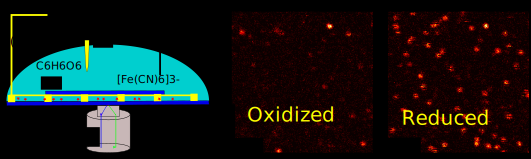
\includegraphics[width=\textwidth]{Scheme_1_setup}
	\caption{Scheme of the confocal and electrochemical setup.
	\textbf{(1)} Objective through which light is irradiated on and collected from the sample.
	\textbf{(2)} Functionalized sample slide with another small glass slide on top the platinum grid.
	\textbf{(3)} Electron mediator solution containing \SI{200}{\uM} ferricyanide, \SI{100}{\uM} ascorbate in PBS (pH 7.4) buffer with a total volume of 4 mL.
	\textbf{(4)} Working electrode (platinum wire) that is in contact with the platinum grid (yellow blocks) with a height of \SI{50}{\um}.
	\textbf{(5)} Saturated calomel reference electrode (SCE).
	\textbf{(6)} The platinum wire (not touching the grid) as counter electrode.
	\textbf{(7)} Potentiostat (Model 800B Series Electrochemical Detector, CH Instruments) to which the electrodes are connected.
	Zoom-in picture shows the functionalization method and the working electrode around it. 
	\textbf{(8, 9)} Confocal scanning images of the surface of the substrate at \SI{100}{\mV} (oxidizing) potential and \SI{0}{\mV} (reducing) potential.
	The spots on the left side (8) are impurities/bleached proteins.
	}
  	\label{sch:setup}
\end{figure}
\paragraph*{Data recording.}
A \SI[product-units=repeat]{20x20}{\um} area of the sample surface functionalized with sparsely distributed ATTO655-labeled azurin was scanned with \SI{50}{\nm} per pixel and with a dwell time of \SI{1}{\ms} per pixel.
A typical fluorescence intensity image can be seen in Scheme \ref{sch:setup}.
A constant potential of \SI{200}{\mV} vs SCE (oxidizing) was applied by the potentiostat and an image of \SI[product-units=repeat]{10x10}{\um} area was taken after \SI{2}{\minute}.
Typically within one minute, the solution potential of the mixture of \SI{0.1}{\mM} ascorbate and \SI{0.2}{\mM} ferricyanide reaches the applied potential.
Another image of this same area was recorded at \SI{0}{\mV} (reducing).
The two images were compared to identify the active molecules, which switch to a bright and dark at the two potentials (Scheme-\ref{sch:setup} (8 \& 9)).
The coordinates of the switching molecules were registered and an automatic recording was started.
For each molecule, time traces were recorded for \SI{30}{\s} at different potentials between \SI{-100}{\mV} and \SI{100}{\mV}.
To observe the dynamics of a single molecule over longer times, time traces were recorded until the dye was  bleached or the protein was denaturated.
Zn-azurin-ATTO655 was used as a control since it does not show switching at the above potentials.
Time traces at the same potentials for the same durations were recorded as for the Cu-azurin.


\paragraph*{Data analysis.}
The measurements resulted in more than a 1000 time traces.
Each time trace contains the absolute arrival times of photons as well as the arrival time with respect to the excitation laser pulse.
This enabled us to extract maximum information from the traces.
To minimize accidental variation and improve efficiency, codes were written (in Python and Matlab) to standardize the analysis of the time traces.
% The codes and data can be found in the given link (will be provided during submission).
Each trace was analyzed in three ways (i) Intensity change points in the time traces were obtained using the Change-Point algorithm\cite{watkins2005detection} provided by prof. Haw Yang 
(Princeton University, USA).
This method is bin-free and does not require any prior knowledge of the underlying kinetics.
It determines the location of intensity changes based on the photon arrival times and the algorithm is recursively applied over the whole time trace to find all the changes.
A Bayesian information criterion is used to find the number of states.
In the present case two states were identified from long time traces of many molecules (2500 change points each) with a reported accuracy of more than \SI{90}{\percent}.
This is in agreement with our expectation of two states, namely a Cu(II)-quenched (low intensity) and a non-quenched Cu(I) state (bright).
Consequently the number of states for the other time traces has been set to two to minimize the computation time.
An example of a trace with change points and its overlap with the real time trace can be seen in Figure-\ref{fig:timetrace}.
(ii) Autocorrelation functions of the time traces were calculated using the SymPhoTime(PicoQuant) software.
(iii) Further analysis of Change-Point outputs and the autocorrelation outputs were performed in Python.
% The details of the code including all the fitting functions can be found in the online repositories (will be provided during submission).


%%%%%%---------------------RESULTS and DISCUSSION-----------------------%%%%%%%%%
\section{Results and discussion\label{sec:results}}
\paragraph*{Time traces at different potentials.}
Active Cu-azurin molecules were identified from their fluorescence intensity images under oxidizing (\SI{200}{\mV}) and reducing conditions (\SI{0}{\mV}).
In reducing conditions, the image contains many bright spots corresponding to Cu(I)-azurin-ATTO655 and more than \SI{90}{\percent} of these molecules are turned off in oxidizing conditions 
(Scheme-\ref{sch:setup}(8)).
The azurins on each sample slide showed active switching during the course of the experiment (up to two days) without any noticeable degradation.
A set of active azurins were marked for recording, and time traces at different potentials (between \SI{-100}{\mV} and \SI{100}{\mV}) were measured on the \texttt{same molecule} 
for \SI{30}{\s}.
Many of the labeled proteins bleached during the recording at the first few potentials, but more than \SI{50}{\percent} of the labeled azurins survived at least five measurements (\SI{150}{\s}  total) at different potentials.
Longer measurements were possible thanks to the scavenging of oxygen in the solution.
Indeed, before recording the time trace, the solution was exposed to a negative potential for at least \SI{1}{\hour}.
Ascorbate is known to  scavenge oxygen\cite{dave1997effectiveness} and get oxidized.
The oxidized ascorbate is then reduced by the electrode and is again available to scavenge other oxygen molecules.
% In addition to the absence of oxygen, the  oxidizing-and-reducing-system (ROXS) mechanism was also at play.\cite{cordes2009on}
The reduction and oxidation of Cu-azurin made the dye switch from bright to dark fluorescent states. Under oxidizing conditions, the dye spent less time in the bright state, and the bleaching rate was reduced.
We could measure some fluorescence time traces for more than \SI{1000}{\s}.\\
%---time trace
\begin{figure}
	\centering
	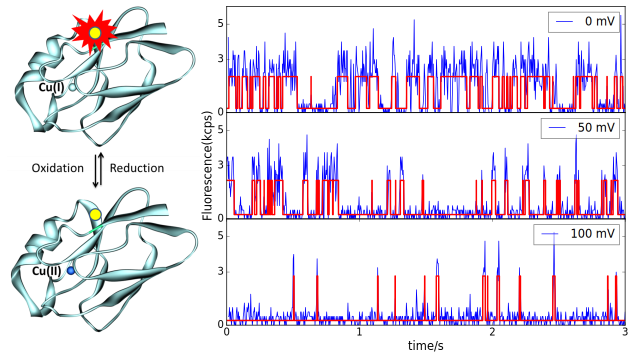
\includegraphics[width=\textwidth]{Figure_1_timetrace_CuAzu}
	\caption{Time traces of the same Cu-azurin-ATTO655 at different potentials (0, 50 and \SI{100}{\mV} with respect to SCE).
	The structure of the protein with properly positioned dye can be seen in the schematic picture in the left.
	In the Cu(II) state (shown as blue dot in the protein structure), the dye is non fluorescent because of FRET and in the Cu(I) state (shown as as a gray dot), the dye is fluorescent. Notice the amount of time the protein spends in the bright and the dark state at different potentials.
	At lower potentials (e.g \SI{0}{\mV}) the protein is bright most of the time because of the higher concentration of reductant.}
	\label{fig:timetrace}
\end{figure}


Figure \ref{fig:timetrace} shows time traces of a single Cu-azurin-ATTO655 molecule at three different potentials. 
The intensity changes from bright to dark and vice versa over time.
In the dark state, the dye fluorescence is quenched by energy transfer to the absorbing Cu(II) center\cite{kuznetsova2006a}.
The high FRET efficiency is due to the small distance of the dye to the absorption center.
This clear distinction between the dark and bright states is important to clearly distinguish redox states, even for low laser power and low signals.
At higher potential (\SI{100}{\mV}), the protein spends most of its time in its dark state and as the potential is lowered, the molecule spends more and more time in its bright state.
Bulk (ensemble) measurements of the fluorescence intensity under completely oxidizing and completely reducing conditions shows \SI{90}{\percent} switching ratio (Figure S\ref{SIfig: switching}) for the lysine-122 labeled Cu-azurin-ATTO655.\cite{nicolardi2012topdown}
In the single-molecule traces in Figure \ref{fig:timetrace}, no clear fluorescence signal from the quenched state could be detected.
However, residual fluorescence from the quenched state can be observed at higher laser power (\SI{0.7}{\uW}) as can be seen in (Figure S\ref{SIfig: lifetime}).
This proves that the observed intensity changes are not due to blinking of the dye, but due to incomplete (\SI{90}{\percent}) quenching by the copper center. 
We also note that the Cu(II)-state has a much shorter lifetime (\SI{0.3}{\ns}) than the Cu(I)-state (\SI{1.9}{\ns}), but still significantly longer than the instrument response function (\SI{0.2}{\ns}). 
Both measurements of intensity and lifetime indicate that the dim state is quenched by energy transfer to Cu(II), in agreement with bulk fluorescence measurements on Cu-azurin.


Figure \ref{fig:timetrace} also shows that bright times shorten at larger electrochemical potential.
This agrees with the higher oxidant concentration in the solution. 
A control study with Zn-azurin-ATTO655 (Figure S\ref{SIfig:tracecomparision} and Figure S\ref{SIfig:fcscomparision}) shows that the dye itself blinks below \SI{40}{\mV}.
Zn-azurin is inert to redox changes and thus the blinking can only originate from the interaction of the dye with the reductant through photo-excited electron transfer.
To exclude redox reactions of the dye itself, we only considered potentials above \SI{40}{\mV} for the Cu-azurin-ATTO655 study.


%Midpoint histogram
\paragraph*{Midpoint potential of single azurins.}
Figure \ref{fig:midpoint}a shows the ratio between the average dark time ($\me{t}_{d}$) and average bright time ($\me{t}_{b}$) plotted against the applied potential.
The relationship of this ratio with the potential is given by the Nernst equation: 
\begin{equation}
	E = E_0 - \frac{k_BT}{n e}\ln\left(\frac{\me{t}_{b}}{\me{t}_{d}}\right)\,
	\label{eq:nernst}
\end{equation}
where $E$ is the applied potential, $E_0$ the midpoint potential, $k_B$ the Boltzmann constant, $T$ the absolute temperature, $n$ the number of electrons involved in the reaction and $e$ the electron charge.
The value of $n$ was found to be $1$ from the data analysis when the slope in the Nernst equation was kept as a free parameter (see Figure-S\ref{SIfig:potential_slope}).
Each color represents a single azurin molecule and the solid line connecting the points is the fit with the Nernst equation.
Labeled proteins surviving at least three potentials above \SI{40}{\mV} were used for the fit.
The potential at which the bright-dark  ratio equals $1$ is the midpoint potential.
The distribution of midpoint potentials (Figure \ref{fig:midpoint}b) from \SI{132}{ molecules} can be fitted by a Gaussian with a center value of $\left<E_0^{SM}\right>=4.5 \pm 1.2~mV$ and a full width half maximum (FWHM) of $\sigma^{SM}=36 \pm 3~mV$. 
The midpoint potentials are similar to previously reported values of $6\pm0.6~mV$ with $FWHM=\SI{150}{\mV}$ where each $E_0$ was calculated from a cluster of about \SI{1000}{ molecules}.\cite{davis2006monitoring}
Another work reported $E_0 = \SI{16}{\mV}$ with low surface coverage (100's of azurins) with a FWHM of \SI{70}{\mV}.\cite{salverda2010fluorescent} 
Recently, for single azurin molecules, a midpoint potential of $E_0=12\pm3$ was reported with a FWHM of \SI{92}{\mV}.\cite{akkilic2014chemically-induced}\\
\begin{figure}
	\centering
	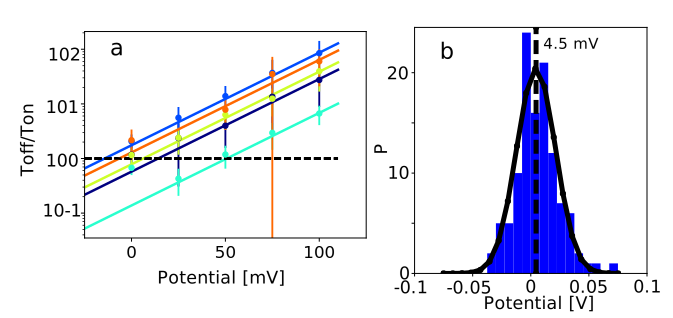
\includegraphics[width=\textwidth]{Figure_2_midpoint}
	\caption{Ratio between bright and dark times as a function of applied potential for the same single azurin.
	Different colors represent different single molecules.
	The line connecting the data points is the Nernst fit with $n=1$ for all the data points above \SI{40}{\mV}.
	The plot at the right is the histogram of midpoint potentials for \SI{132}{ molecules} with a Gaussian fit with a center value of \SI{4.5}{\mV} with respect to the calomel electrode.}
	\label{fig:midpoint}
\end{figure}

The distribution of midpoint potentials we find for single azurin is narrower (FWHM \SI{36}{\mV}) than in earlier measurements. We attribute this narrow distribution to a weaker interaction with the surface. Indeed, in our experiment, the proteins were functionalized through a PEG tether with a length of ${\sim}\SI{20}{\nm}$ itself attached to the surface by a NeutrAvidin. The total tether length is much longer than in earlier experiments, where the azurin was either non-specifically attached to the surface, or attached through a very short linker (\SI{<1}{\nm}).
In addition, the PEG passivation of the glass surface minimizes the interaction of the protein with the surface. Indeed, no protein was found to bind to the surface if the neutravidin was taken out, showing the absence of non-specific interactions.

%====================Many single-molecule on-off histogram and their rates=================
\paragraph*{Redox reaction rates from histograms of bright and dark times.}
\begin{figure}
	\centering
	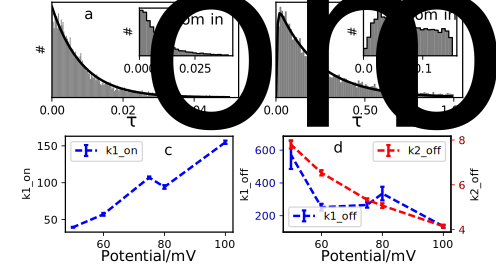
\includegraphics[width=\textwidth]{many_sm_hist}
	\caption{\textbf{Electron transfer rates (many molecules)} The histogram of bright times (a) and dark times (b) obtained from 132 single-Cu-azurin-ATTO655 molecules at \SI{100}{\mV}. The inset shows a magnified part for short times.
	The bad fit of the histogram of bright times with a single-exponential function shows its  non-exponentiality.
	Similarly the histogram of dark times shows non-exponential decay but with a buildup (rise time) at the begining.
	A possible interpretation is that reduction of Cu-azurin occurs through an intermediate step while for oxidation no intermediate state is observable.
	(c) Oxidation rate constant as a function of potential. 
	(d) Reduction rate constant as a function of potential: blue points correspond to the faster rate constant (rise, $k_2$) while the red points represent the slow rate constant ($k_3$).}
	\label{fig:many_sm_hist}
\end{figure}
The number of bright-dark switching events for a single azurin molecule was limited by fluorescence bleaching and led to noisy distributions.
For this reason we first analyzed the overall distribution of bright- and dark-times of all the single molecules obtained at a certain potential, which basically can be considered as an ensemble measurement.
Figure \ref{fig:many_sm_hist}(a) shows the histogram of bright-times at \SI{100}{\mV} and the solid line is the fit of a single exponential with a time constant ($k_{1}$) of \SI{155}{\per\s}.
The on-time represents the time the protein spends in the reduced state before getting oxidized according to the following reaction scheme:
\begin{align}
	\ch{!(bright)(Cu(I)Az) + ox <=>[ $k_1$ ][ $k_{-1}$ ] !(dark)(Cu(II)Az) + red }
	\label{eq:oxidation}
\end{align}
In contrast, the distribution of bright-times shows a maximum with a buildup and decay (Figure \ref{fig:many_sm_hist}(a)).
The inset with binning time \SI{5}{\ms} clearly shows that the probability of finding very short bright-times is relatively small.
This distribution can be explained with the Michaelis-Menten mechanism:
\begin{align}
	\ch{!(dark)(Cu(II)Az) + red <=>[ $k_2$ ][ $k_{-2}$ ] !(dark)(Cu(II)Az.red) -> [ k3 ] !(bright)(Cu(I)Az) + ox}
	\label{eq:reduction}
\end{align}
where $k_2$ is the pseudo-first order rate constant, which depends on the concentration of reductant and $k_3$ is the zero order rate constant, which should be independent of the concentration of the substrate.
When assuming $k_{-2}=0$, the probability distribution of bright times is given by\cite{lu1998single-molecule}
\begin{equation}
	P(t_{d}) = \frac{k_2k_3}{k_3-k_2} [exp(-k_2t_{d})-exp(-k_3t_{d})]
	\label{eq:2exp_risetime}
\end{equation}
At \SI{100}{\mV}, $k_2$ for the reduction is \SI{4.1}{\per\s} while $k_3$ is \SI{135}{\per\s}.
The data doesn't match with a single component distribution, which is not surprising as the distribution is built from many single azurins and each azurin has its own decay.
Similar to the distribution in midpoint potential, the non-exponential decay is a reflection of the statistical heterogeneity among the azurins.

The oxidation and reduction rates were determined at different applied potentials.
As expected, the rate constant for the intermediate complex formation ($k_2$) is dependent on the substrate concentration and thereby the potential while the rate constant for electron transfer in the intermediate is independent of the potential (Figure \ref{fig:many_sm_hist}(c)).
The rate of complex formation can be modeled as:
\begin{equation}
	k_3 =k_3^0\times[R] \text{ and } k_1 =k_1^0\times[Ox]
	\label{eq:rate_complex}
\end{equation}
\begin{equation}
	[R] = \frac{R_0exp(\frac{E_0^R-E}{0.059})}{1+exp(\frac{E_0^R-E}{0.059})}
	\text{ and } [Ox] = \frac{O_0}{1+exp(\frac{E_0^O-E}{0.059})}
	\label{eq:conc_potential}
\end{equation}
$[R]$ is the concentration of reductant (equivalent to ``substrate'' in enzymology), $R_0$ is the starting concentration of reductant which is equal to the concentration of ascorbate in this case, $E_0^R$ is the standard redox potential of ascorbate that is \SI{30}{\mV} and $E$ is the applied potential. The value $0.059$ stands for $\frac{RT}{nF}$ similar to the slope in the Nernst equation(Eq. \ref{eq:nernst}) with $n=1$.
Similarly $[Ox]$ represents the concentration of the oxidant (ferricyanide) at different applied potentials.
The maximum rate constant of reduction ($k_3^0$) was obtained to be $3.3\times10^5~M^{-1}s^{-1}$ while the maximum rate constant of oxidation was $1.3\times10^8~M^{-1}s^{-1}$.


However, Terentyeva et al. have shown that the presence of a rise time in the bright-time distribution can be an artifact in the changepoint analysis.
Our initial simulations and change point analysis indicates the underestimation of short dark times but not the extent that can give a rise time.
Our interpretation of the build-up in the histograms is thus under further investigation.

%==================Dynamics: Single-azurin over time===================
\paragraph*{Dynamical heterogeneity.}
After studying ${\sim}150$ single azurins together in an ensemble fashion, we investigated single azurins for as long as their fluorescence survived.
Figure \ref{fig:long_azurin_trace} shows the statistics of a single azurin at \SI{100}{\mV} that survived for \SI{\sim350}{\s}.
Two different parts of the original time trace (\ref{fig:long_azurin_trace}C), indicated by colored blocks, are magnified and shown in Figure \ref{fig:long_azurin_trace}A and B.
The two zoomed-in traces have very different bright-dark characteristics.
The one on the left has short bright-times and long dark-times while the one on the right has long bright-times and short dark-times.
The full time trace was divided into small parts and the average was calculated over every $10$ consecutive bright and dark times (Figure \ref{fig:long_azurin_trace}E,G).
We averaged over 10 points to reduce noise (see SI Fig S\ref{SIfig: N_avgpoints_vs_fwhmwidth}) and highlight the difference between the two parts of the trace.
Unlike random (Gaussian) noise, spikes and correlated high-low events are observed on the trace, which is also reflected in the density of points per unit time.
Longer bright and dark times result in a lower density of points.
The histograms of bright and dark times are shown on the left side of the trace without any averaging and the fit is shown with a single exponential function.
The distribution of dark times is clearly non-exponential as can be seen from the big deviation from the exponential fit.
Surprisingly, the histogram of bright times fits well with an exponential function even though the trace of bright times shows clear variation. 
The trace of midpoint potential (Figure \ref{fig:long_azurin_trace}I) is calculated through the Nernst equation for each point on the trace and with the applied potential.
The midpoint potential in the trace also fluctuates in a non-Gaussian way which can also be seen in the shape of its distribution (Figure \ref{fig:long_azurin_trace}H) with an average value of \SI{42.2}{\mV}.
%long_azurin_trace
\begin{figure}
	\centering
	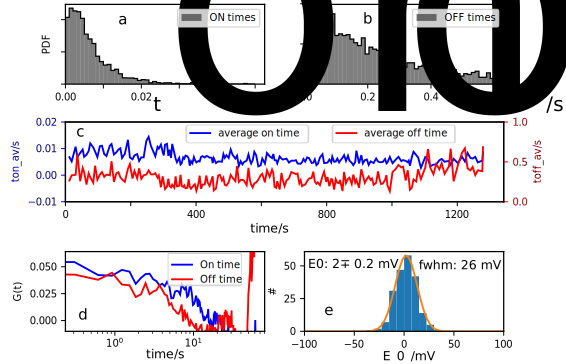
\includegraphics[width=\textwidth]{long_azurin_trace}
	\caption{\textbf{Dynamic heterogeneity.}
	A long time trace (C) of Cu-azurin-ATTO655 at \SI{100}{\mV} with zoom-in (A, B) at different points of its time course.
	Variation of bright times (E) and dark times(G) of the same azurin with their histogram on the left.
	The times were averaged over every ten consecutive ones to get rid of noise and for easy visualization.
	The trace of midpoint potential(I) calculated from the bright- and dark-times and the the histogram(H) of midpoint potential is shown on its left with an average value of \SI{42}{\mV}.
	}
	\label{fig:long_azurin_trace}
\end{figure}


The heterogeneity in the bright and dark times is related to the heterogeneity in the rate of electron transfer, particularly the longer times, which presumably is the rate of intermediate-complex formation.
The first explanation of heterogeneity we should consider is the effect of the surface.
Previous studies have shown that the azurin can stick to hydrophobic surfaces through the different hydrophobic patches on the protein surface.\cite{patil2010visualizing,salverda2010fluorescent,akkilic2014chemically-induced}
However, special care was taken to keep the protein as far as possible from the surface through a long (\SI{\sim20}{\nm}) PEG-linker, and to passivate the surface with short PEG ligands.
Indeed, no azurin was found attached to the surface of the substrate when the labeled azurin was flown onto the surface without NeutrAvidin or Biotin (everything else in the functionalization method kept the same) indicating the absence of non-specific interactions between the protein and the surface.
The narrow distribution (narrower than any previous measurements) of midpoint potentials among the 132 single azurins (Figure \ref{fig:midpoint}) also confirms the absence of interaction with the surface.
From these observations, we conclude that the surface contribution to the heterogeneity can be ignored.
We can also rule out concentration fluctuations of reductant and oxidant, as the solution potential is precisely controlled by the potentiostat.


The heterogeneity in the rates can now only be attributed to conformational changes of the protein.
Midpoint potential changes (\SI{<4}{\kJ\per\mole}) are much smaller than the changes in the free energy (\SI{-23}{\kJ\per\mole}, $\Delta{G}=-nEF$) related to the change in the oxidation state of azurin.
Such small changes can be attributed to subtle changes in the structure of the protein, each of these sub-structures are called conformational sub-states.

%XXXX Think about the argument XXXX


The protein remains in certain conformational sub-states for a duration of time, which can be observed in the time trace.
A short bright-time followed by a short bright-time represents one state while a long bright-time followed by a long bright-time represents another sub-state.
The residence time in each of these conformational sub-states can be characterized by autocorrelating the time trace of bright and dark times (Figure \ref{fig:Dynamic_corr} A).
The characteristic correlation times are in the order of $1-10$ of seconds, and the correlation times for bright and dark times are different.
The signature of changes in the reaction rates can also be seen in the fluorescence intensity correlation (Figure \ref{fig:Dynamic_corr}B) with a decay at round \SI{\sim50}{\s} which basically has both the information about the redox reaction rates.
However, the individual rates related to bright and dark times can not be extracted from the intensity correlation unless the underlying kinetics is known.
\begin{figure}
	\centering
	\includegraphics[width=\textwidth]{Dynamic_corr}
	\caption{\textbf{Dynamic correlation.} (A) Autocorrelation of the bright and dark times in the trace showed in Figure \ref{fig:long_azurin_trace}E, G. (B) Autocorrelation of the intensity trace shown in Figure \ref{fig:long_azurin_trace}C. The inset shows the zoom-in of the intensity correlation in the longer time scale.}
	\label{fig:Dynamic_corr}
\end{figure}


In the 1980s, conformational sub-states were observed in the association and dissociation of carbon monoxide (CO) with myoglobin in bulk experiments where sub-populations were found with different binding rates of CO.
The time scales of binding varied from microseconds to seconds, indicating large variations of the reaction rate with the possible conformations of myoglobin.
Indication of heterogeneity has also been observed for single enzymes with some success ($\beta$-galactosidase, flavoenzymes)\cite{lu1998single-molecule,kou2005single-molecule,english2006ever-fluctuating}.
Here the dynamic rates have been observed for single azurin molecules in the time scale of tens of seconds, which varies from protein to protein as can be seen in SI Fig. S\ref{SIfig:Dynamic_corr_many}
More examples of azurin molecules with their intensity traces and traces of bright and dark times can be seen in SI Fig. S\ref{SIfig:dynamic_trace_steps}, S\ref{SIfig:dynamic_Point_20_75mV_S105}, S\ref{SIfig:dynamic_Point_21_75mV_S105}, which can give a feeling of the different dynamics and their irreproducibility within the time of observation.
As the oxidation and reduction occur in the range of hundreds of milliseconds, conformational changes at shorter time scales cannot be determined by this method.
Among the proteins that were recorded, no two proteins seemed to have the same dynamics, indicating the vast number of conformational sub-states that a protein can be in.
It was thus impossible to build an experimental map of such a large number of states.

% Some proteins were also found to have no decay in the correlation (e.g. Figure \ref{fig: N_avgpoints_vs_fwhmwidth}C), primarily indicating the absence of dynamical heterogeneity.
% Looking back at the histogram of midpoint potentials obtained from 132 single azurins, can the contribution of dynamical heterogeneity be estimated to the distribution (fwhm=\SI{36}{\mV}) for all the single-azurins.

% Also midpoint potentials were calculated from each average bright and average dark times using the Nernst equation(\ref{eq:nernst}).
% As both bright-and dark-times change over time, the midpoint potential too changes over time. 
% The distribution of $E_0$ shows a center value of $2\pm0.2~mV$ with a fwhm of \SI{26}{\mV}.
% This distribution of midpoint potential of a single-azurin over a long time is similar to the value of \SI{36}{\mV} obtained from many single-azurins.
%=================CONCLUSION==================
\section{Conclusion}
The results presented here show how to controllably switch the solution potential and determine the switching ratio of redox active azurin.
By introducing a non-interacting surface and a long linker, we obtained a narrow distribution of midpoint potentials.
The distribution over many single-azurin was found to be close to the distribution of a single-azurin over a long time.
The rate of intermediate formation for the reduction process that has been observed is consistent with a Michaelis-Menten mechanism.
The intermediate formation for the oxidation was too fast to detect with our signal-to-noise ratio.
In principle, similar measurement at higher laser power and for many molecules should enable the detection of the intermediate if there is any.
For the first time, correlated dynamic heterogeneity is observed in the complex formation between azurin and its redox partners.
We proved the presence of dynamic heterogeneity and presented several ways to characterize it: through the non-exponential distribution of reaction rates, the correlations of the redox times, and through the long correlation times found in fluorescence intensity correlation.
Our study proves the presence of conformational heterogeneity in an electron-transfer protein, and makes it plausible that similar heterogeneity may be a general feature in all types of enzymes and proteins.
%================================= SUPPORTING INFORMATION ========================================
\graphicspath{{chapters/c4_azurin_sm/si/}}
%=====================METHODS AND FIGURES===========================
\section{Supporting Info}
%Peak separation
\begin{figure}
  \centering
  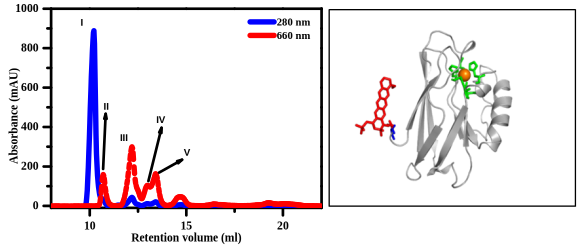
\includegraphics[width=0.8\textwidth]{peak_separation}
  \makeatletter
  \renewcommand{\fnum@figure}{\figurename~S\thefigure}
  \makeatother
  \caption{Peak separation: (a) Elution profile of Cu azurin sample after labeling and removal of free dye.
  \SI{280}{\nm} absorption that tells the presence of protein is shown in blue and \SI{660}{\nm} absrption that tells the presence of  dye is shown in red.
  The protein structure with the dye at Lys corresponding to peak-III is shown in the right. 
  {A proper structure will be replaced}}
  \label{SIfig: peak_sep}
\end{figure}
% \pagebreak
%==================BULK Switching=========================
\paragraph*{Fluorescence switching in bulk} Fluorescence measurements in bulk of different peaks of azurin-ATTO655 sample (Figure S\ref{SIfig: peak_sep}) were carried out to determine the FRET switching ratio.
The measurements were done in Cary Eclipse Spectrometer (Varian Inc. Agilent Technology, USA).
A \SI{50}{\nM} sample was excited with \SI{665}{\nm} and intensity was monitored above \SI{675}{\nm}.
Sodium ascorbate (reductant) and pottasium ferricyanide (oxidant) were added alternatively.
Among all the labeled position, peak-III showed maximum switching ratio and it's intensity change can be seen in Figure S\ref{SIfig: switching}.
Similarly Zn Azurin-ATTO655 showed little or no change in intensity.
\begin{figure}
  \centering
  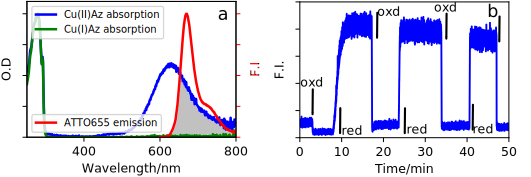
\includegraphics[width=\textwidth]{spectral_overlap_switching}
  \makeatletter
  \renewcommand{\fnum@figure}{\figurename~S\thefigure}
  \makeatother
  \caption{Spectral overlap and Bulk switching: (a) Absorption spectrum of Cu(II)azurin (blue), Cu(I)azurin (blue).
  The emission spectrum of ATTO655 (red) has a good overlap with the absorption of Cu(II)azurin to show high FRET. 
  (b) Fluorescence intensity of \SI{50}{\nM} CuAzurin-ATTO655 shows high intensity in the presence of reductant and low 
  intensity with oxidant.
  The switching ratio comes to be \SI{90}{\percent} satisfying the requirement for single-molecule FRET.}
  \label{SIfig: switching}
\end{figure}
%==================time trace Zn and Cu azurin=================
\begin{figure}
  \centering
  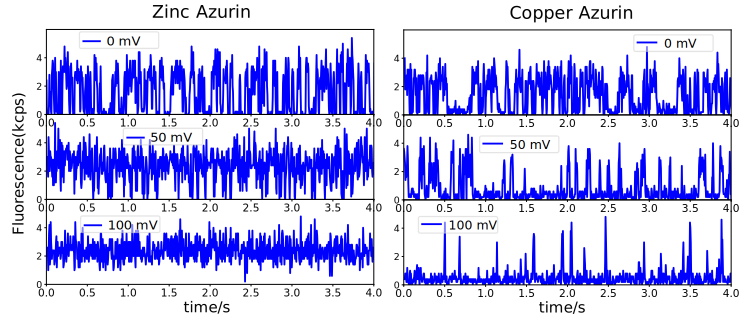
\includegraphics[width=\textwidth,keepaspectratio]{SI_timetrace_Zn_Cu}
  \makeatletter
  \renewcommand{\fnum@figure}{\figurename~S\thefigure}
  \makeatother
  \caption{Time traces of Zn Azurin (left) and of Cu Azurin(right) labeled with ATTO655 at different potential. 
  Above \SI{40}{\mV}, Cu-Azurin show swiching in the intensity due to changes in the oxidation state of the Copper metal center and below \SI{40}{\mV}, triplet blinking contributes to the switching as can be seen in the redox inactive Zn-Azurin.
  To keep the analysis simple, time traces above \SI{40}{\mV} were choosen for Cu azurin}
  \label{SIfig:tracecomparision}
\end{figure}
%===================lifetime and switching ration from time trace================
\begin{figure}
  \centering
  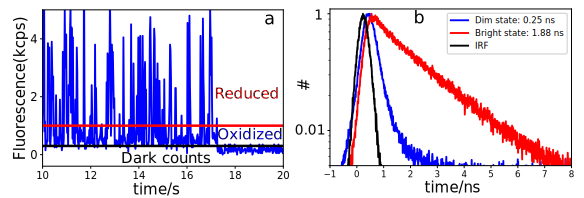
\includegraphics[width=\textwidth]{lifetime}
  \makeatletter
  \renewcommand{\fnum@figure}{\figurename~S\thefigure
}  \makeatother
  \caption{Single-molecule azurin switching and lifetime. (a) Time trace of a single Cu azurin at \SI{50}{\mV} with a binning time of \SI{50}{\ms}.
  Notice the three different labels indicated in the figure. Bright (Cu(I)) state as above the red line, oxidized state is between red and black and Dark counts are below the black line. The fact that the molecule doesn't go to the dark count label before being bleached shows that the transitions are due to Copper oxidation switching rather than triplet blinking of the dye.
  Once the fluorophore is bleached, no transitions were observavable.
  (b) The lifetime histogram corresponding to bright state (red), oxidized state (blue) and instrument response function (black).
  The lifetime of oxidized state is much shorter than the reduced state due to FRET quenching.}
  \label{SIfig: lifetime}
\end{figure}
%=====================FCS comparision=========================
\begin{figure}
  \centering
  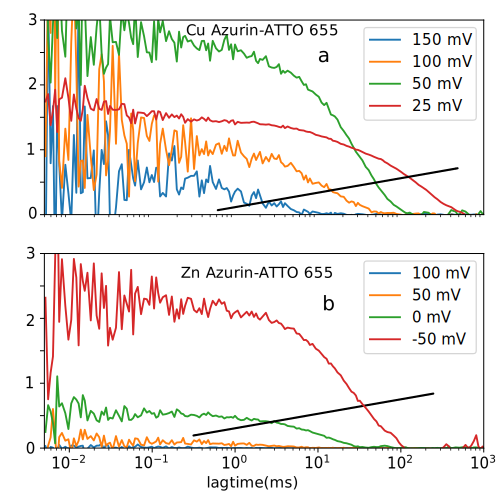
\includegraphics[width=\textwidth]{fcs_comparision}
  \makeatletter
  \renewcommand{\fnum@figure}{\figurename~S\thefigure}
  \makeatother
  \caption{Autocorrelation of time traces of Cuazurin-ATTO655 (a) and Znazurin-ATTO655 at different potential. 
  At lower potential, Cuazurin-ATTO655 has longer correlation time (on time) which shows that the molecule spends more time on the Cu(I) state.
  But below \SI{50}{\mV} the dye (ATTO655) starts to show triplet blinking.
  As potential is lowered the triplet blinking dominates.
  The Cu azurin study is focussed in the safe window of potential more than \SI{40}{\mV} where triplet blinking is absent.}
  \label{SIfig:fcscomparision}
\end{figure}
%===============================Slope: Nernst equation==================================
\begin{figure}
  \centering
  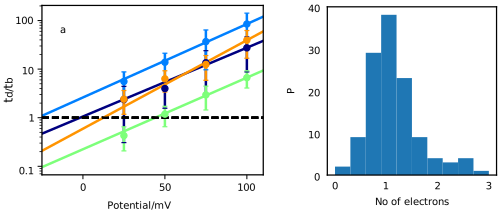
\includegraphics[width=\textwidth,keepaspectratio]{SI_potential_slope}
  \makeatletter
  \renewcommand{\fnum@figure}{\figurename~S\thefigure}
  \makeatother
  \caption{Fitting with Nernst equation with slope as variable parameters for  (a) Cu-Azurin ATTO655. 
  (b) The corresponding histogram of slopes obtained from the fitting shown in the left.T
  he distribution of slope is centered around \SI{59}{\mV} indicating that Cuazurin switching  involves only one electron.}
  \label{SIfig:potential_slope}
\end{figure}
%===================================Rate fit at all potential=============================
\begin{figure}
  \centering
  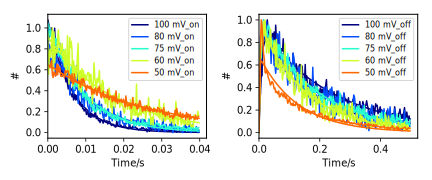
\includegraphics[width=\textwidth]{rate_fit_all_potential}
  \makeatletter
  \renewcommand{\fnum@figure}{\figurename~S\thefigure}
  \makeatother
  \caption{(a) Fitting of $on$ time distribution with monoexponential at different potential.
  (a) Fitting of $off$ time distribution with bi-exponential equation with rise time as shown in the main text at different potential.
  The output rate constants were plotted against potential (see main text)}
  \label{SIfig: rate_fit_all_potential}
\end{figure}
%===================================No of averaging points=================================
\begin{figure}
  \centering
  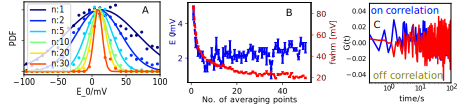
\includegraphics[width=\textwidth]{N_avgpoints_vs_fwhmwidth}
  \makeatletter
  \renewcommand{\fnum@figure}{\figurename~S\thefigure}
  \makeatother
  \caption{\textbf{No correlation dynamics.} Variation of midpoint potential and fwhm with the number of on and off times taken for averaging for the long trace shown in the main text (Figure-\ref{fig:long_azurin_trace}). At around $20~$ events, both $E_0$ and fwhm reaches palteu.
  The averaging of on-time and off-times for correlation and midpoint distribution were done every $20$ events.}
  \label{fig: N_avgpoints_vs_fwhmwidth}
\end{figure}
\paragraph*{}
\begin{figure}
  \centering
  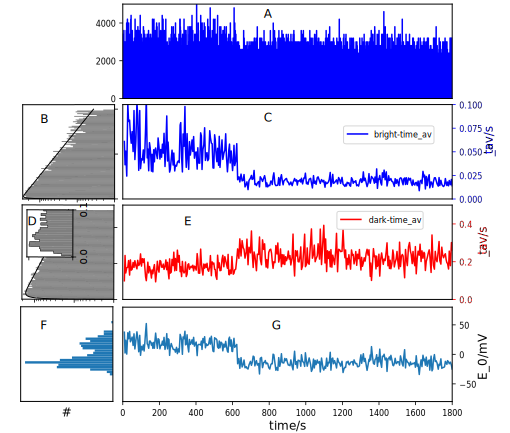
\includegraphics[width=\textwidth]{dynamic_trace_steps}
  \caption{\textbf{Two conformational state dynamics}}
  \label{SIfig:dynamic_trace_steps}
\end{figure}
%============on-off 2D histogram=============
\begin{figure}
  \centering
  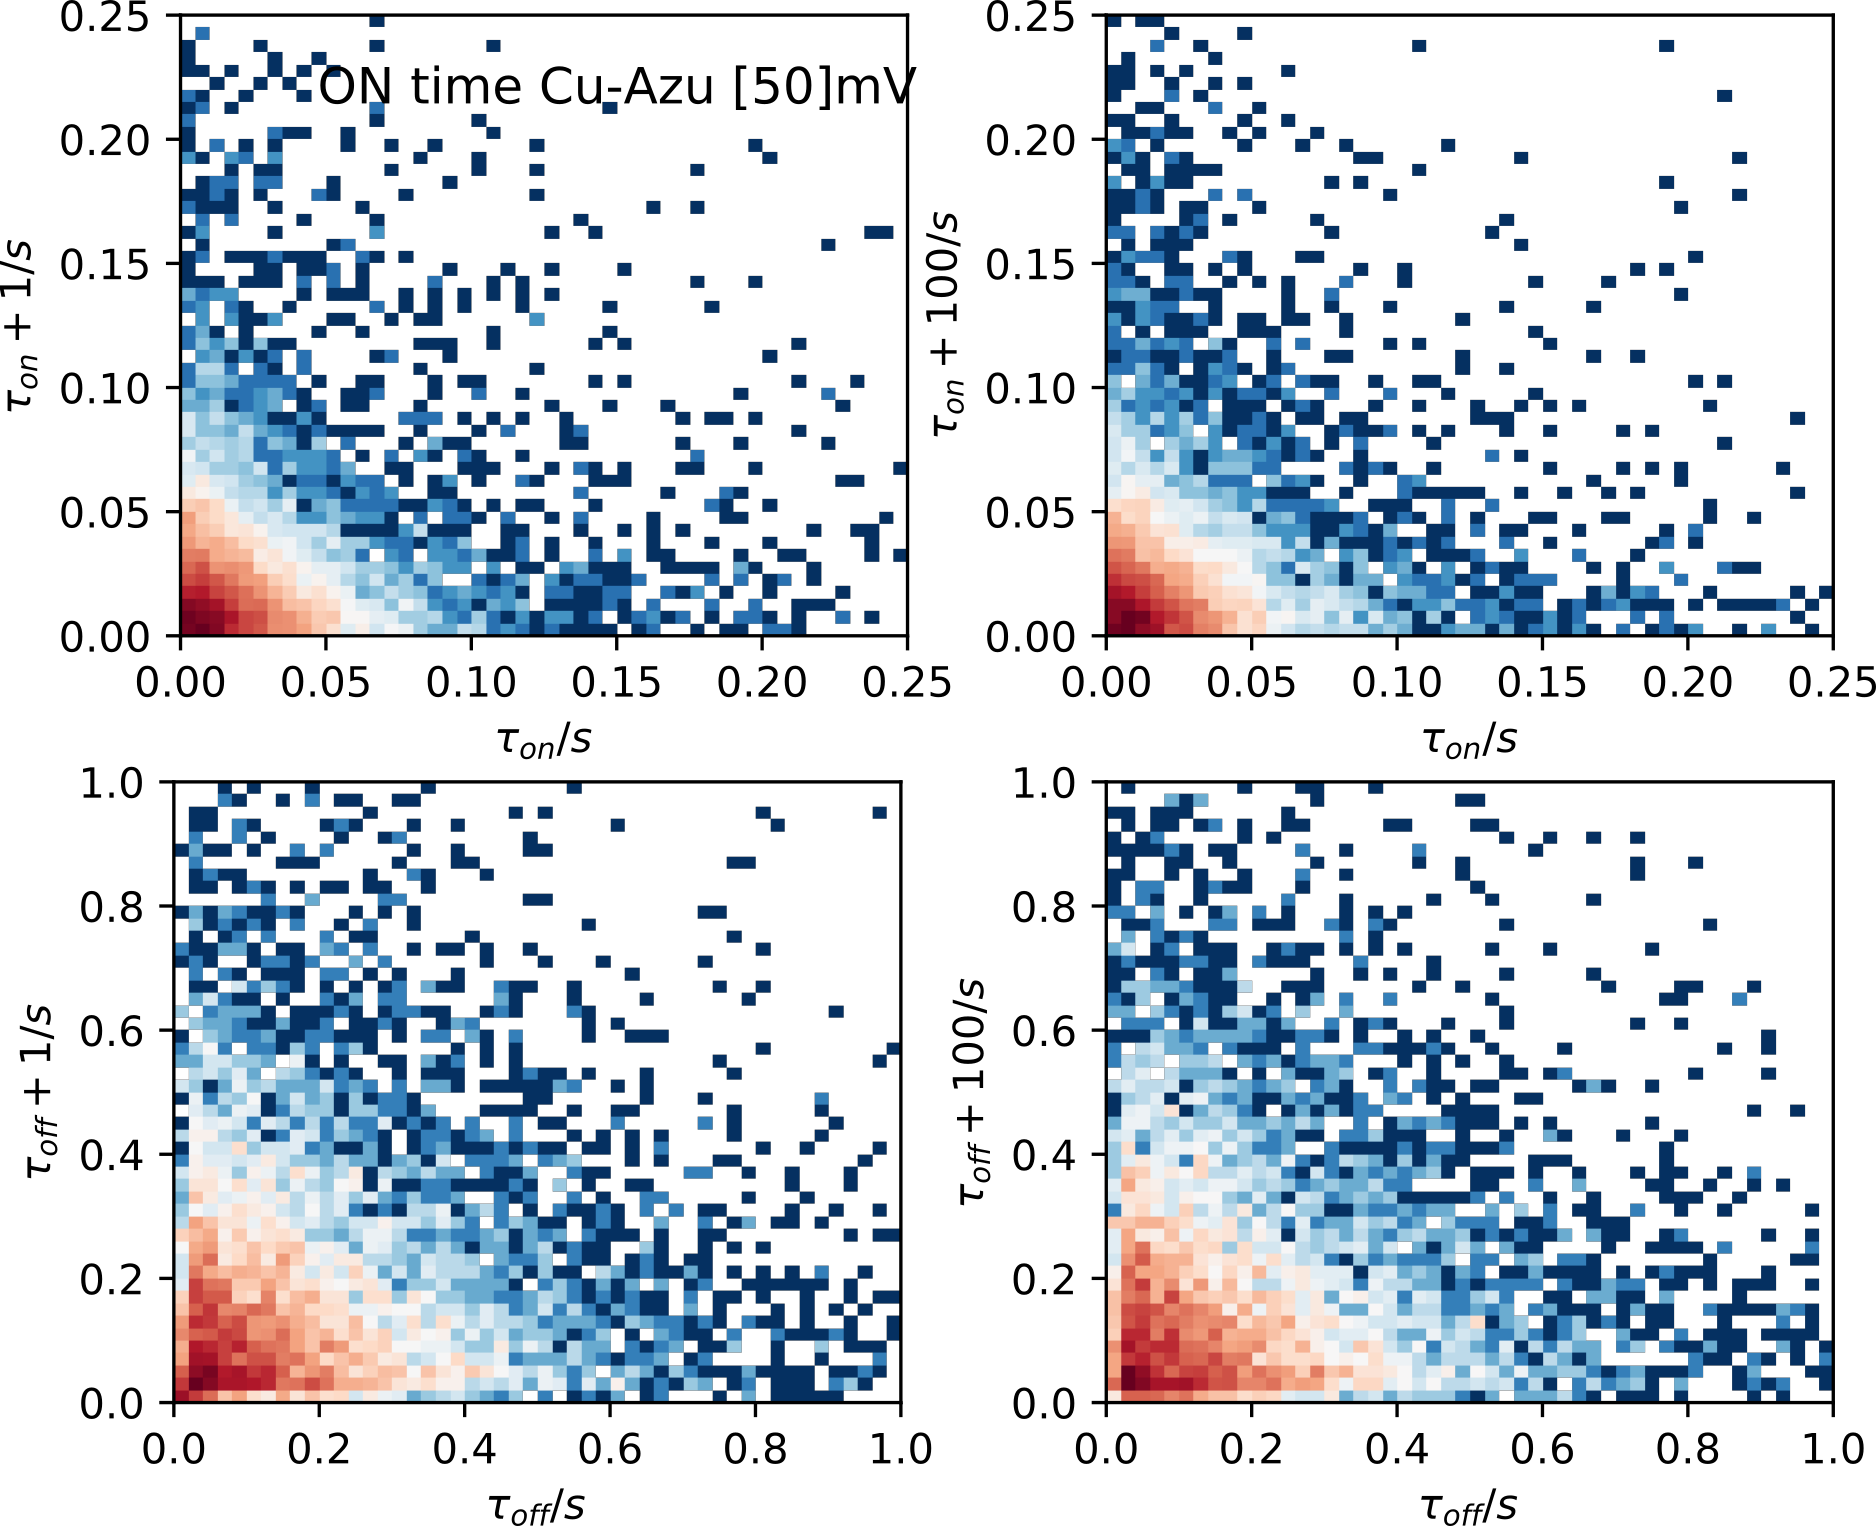
\includegraphics[width=\textwidth]{Figure_4_on_off_2D_100mV}
  \caption{\textbf{2D histogram: Cu-Azurin.}Two-dimensional correlation plot of a single azurin at \SI{50}{\mV} of(a) adjacent waiting time for oxidation ($t_{n}~and~t_{n+1}$) (b) two waiting times at a large separation of 100 ($t_{n}~and~t_{n+100}$) (c) The difference two dimensional histogram of (a) and (b).}
  \label{SIfig:onoff2D}
\end{figure}

\begin{figure}
  \centering
  \includegraphics[width=\textwidth]{dynamic_Point_20_75mV_S105}
  \caption{\textbf{dynamic Point 20 75mV S105}}
  \label{SIfig:dynamic_Point_20_75mV_S105}
\end{figure}
\begin{figure}
  \centering
  \includegraphics[width=\textwidth]{dynamic_Point_21_75mV_S105}
  \caption{\textbf{dynamic Point 20 75mV S105}}
  \label{SIfig:dynamic_Point_21_75mV_S105}
\end{figure}
\begin{figure}
  \centering
  \includegraphics[width=\textwidth]{Dynamic_corr_many}
  \caption{\textbf{More examples of Dynamic correlation.} 
  }
  \label{SIfig:Dynamic_corr_many}
\end{figure}
% \references{chapters/c4_azurin_sm/azurin}
% %======== BIBLIOGRAPHY ===========
\thumbfalse
\chapter*{Bibliography}
\addcontentsline{toc}{chapter}{Bibliography}
\references{bibliography}
% %======== Conclusion and summary =========
\chapter*{Conclusion and outlook}
\label{ch:conclusion}
\markboth{Conclusion}{}
\addcontentsline{toc}{chapter}{Conclusion and Outlook}

% \paragraph*{General conclusion}
This thesis is focused on both the methodology and applications of single-molecule fluorescence. The first three chapters deal with fluorescence enhancement by single gold nanorods which allow single-molecule investigations of optical absorbers with low quantum yield. In the second part, we study electron transfer in single metalloproteins. Here we conclude by summarizing the important outputs of the thesis, possible applications and prospects for future experiments.


\paragraph*{Enhanced FCS}
Enzymatic reactions occur in micromolar to millimolar concentrations.
We demonstrated a plasmonically enhanced fluorescence method to observe single molecules at a higher density of molecules on a lipid bilayer.
A resonant gold nanorod squeezed the electromagnetic energy into a thousand times smaller volume than the diffraction limit of an optical microscope.
We functionalized the bilayer with a high quantum yield dye to characterize both near-field and far-field of the nanorod antenna from the same measurement.
The intensity fluctuations due to the diffusion of the emitters were characterized by fluorescence correlation spectroscopy.
Two diffusion times were obtained from the correlation curve corresponding to the near field and far field.
The near-field volume could directly be estimated from the diffusion times and the known diffusion coefficient in the lipid bilayer.
The lifetime of the enhanced fluorescence was shortened by the nanoantenna.
The correlation amplitude improved by more than an order of magnitude by correlating photons with ten times shorter lifetimes than the un-enhanced fluorescence.
We also functionalized the bilayer with labeled protein and observed enhanced correlation without any physical or chemical harm to the biomolecules.


Our experiment was a preliminary demonstration of enhanced fluorescence correlation spectroscopy and characterization of near-field.
A more application-oriented approach would be to use a dye with a low quantum yield.
Two immediate benefits with weak emitters are: i) fluorescence can be enhanced by three to four orders of magnitude providing high contrast against the far-field, ii) low fluorescence background from the far-field will cause a mild reduction on the correlation amplitude.
Furthermore, nanorods with a surface plasmon at longer wavelength can be used for better fluorescence enhancement and lower natural fluorescence background inside a cell.
In addition to its bio-mimicking function, a lipid bilayer also provides a surface for anchoring biomolecules.
Enzymes and proteins can slowly diffuse in the near-field while we observe their biological activity.
For cellular membranes, the diffusion in the near-field could reveal the patchy domains at high resolution.


\paragraph*{Transient Binding}
In the Chapter 2, we obtained distributed enhancement factors for freely diffusing dyes around a gold nanorod.
Strong inhomogeneity of the electric field around a plasmonic nano-antenna leads to a large variation in enhancement.
We demonstrated a DNA-based transient binding method to observe fluorescence from a fixed point on the gold nanorod.
Many single molecules were observed, one at a time with the same enhancement factor.
The long persistence length of DNA allowed us to fix the position of the emitter.
We controlled the average number of binding sites down to one per gold nanorod with proper passivation of the gold surface.


The rich and robust chemistry of DNA allows us to control distance and binding energy efficiently.
One of the challenges in plasmonic enhancement is to re-construct a three-dimensional map of fluorescence enhancement (or electric field) around a nano-antenna.
With high spatial (0.35~nm resolution per DNA base) control of emitters by DNA, an experiment can be envisioned to transiently bind different lengths of imager (emitter with a short strand DNA) and construct a 3D map using the principles of super-resolution.
As DNA-technology is bio-inspired, plasmonics with DNA can be a natural choice to perform enhancement experiments inside living cells.


\paragraph*{Bin-free analysis}
Intensity or number of photons per unit time (binning time) is a typical quantity used to characterize fluorescence.
Such binned traces give accurate dynamics if the binning time is shorter than the underlying time of intensity fluctuation.
In addition, a high signal to noise ratio is required to get better accuracy of the dynamic parameters.
What if the underlying kinetics is unknown? What binning time should be chosen?
With different binning times, we observed different enhancement factors for the diffusion of dyes in the near field of a gold nanorod.
Accurate estimation of the enhancement factor would help in characterizing the plasmonic effect on the fluorophores.
In this chapter, we proposed a binning-free method with the delay time between two consecutive photons.
Numerical solutions were obtained for the distribution of inter-photon times for the static and dynamic intensities arising from different numbers of molecules and different excitation-detection profiles.
Transient binding on a gold nanorod and diffusion in a bilayer were satisfactorily predicted from their inter-photon times.
For free diffusion in the bilayer, accuracy of our model proved to be better at higher numbers of molecules.
Similar analysis is being carried out for enhanced fluorescence.
We hope to devise a more general binning-free method to characterize fluorescence dynamics.


\paragraph*{Electron transfer in azurin}
Do enzymes and proteins fluctuate in their structure? In the final chapter, we monitored electron-transfer rates of single azurins as a function of time.
Dynamic heterogeneity was observed from the analysis of time traces, histograms of lifetimes of bright and dark states, and correlation of bright and dark times.
Non-exponential (more than two) distributions of bright and dark times indicated distributions in the electron-transfer rates.
As the electron-transfer rates are monitored in steady state, their variation in activity were attributed to different conformations of azurin.
The decay in the correlation of dark and bright times indicated the correlated variation in their electron-transfer rates.
In simple terms, a longer bright time was followed by a longer bright time and a shorter bright time was followed by a shorter bright time.
The decay time in the correlation gives the duration for which an azurin retains a certain conformation.
No two azurin molecules showed the same values of dynamic correlation indicating the large number of conformational substates a protein can possess.
We suppose such changes come from the movement of domains in a protein where weak interactions like hydrogen bonding and hydrophobic interactions give a compact form to a long peptide chain. 


Though we are confident about the presence of substates in azurin, the reason why proteins change their conformations is an open question.
No computational or theoretical model to the best of our knowledge has predicted dynamic correlations on the time scale of seconds.
Azurin is a relatively small and stable protein.
From the presence of heterogeneity in azurin, it is tempting to assume a presence of conformational substates in other proteins as well.


We performed the electron transfer experiment \textit{in vitro} on a non-interacting functionalized glass substrate.
To convince the generality of dynamic heterogeneity, single-enzyme experiments can be performed in biological-mimicking structures like lipid vesicles where interaction from external sources can be minimized.
\chapter*{Summary}
\label{ch:Summary}
\markboth{Summary}{}
\addcontentsline{toc}{chapter}{Summary}

%\paragraph*{General motivation: 1 page}
Absorption of light by organic materials at a particular wavelength followed by emission of light at longer wavelengths is called fluorescence.
% When a sample is illuminated by light of a given wavelength, it often emits light at longer wavelengths. This phenomenon is called fluorescence.
Fluorescence is highly selective and presents negligible background for properly purified samples. These features enable the detection of single molecules, even when they are surrounded by billions of other, non-fluorescent host molecules.
Detailed kinetics and statistical distributions, which are blurred in the averaged ensemble measurements, become directly accessible in single-molecule measurements.
Chemical reactions that cannot be synchronized (asynchronous reactions) and the associated pathways can be studied in real time with single molecules.
In the last two decades, single molecules have revealed detailed biomolecular dynamical processes such as enzyme kinetics, protein energy landscape, protein folding kinetics, breaking of chemical bonds, rare and transient events, and more.
Digital blinking in the fluorescence of single molecules has been used to locate molecules with nanometer accuracy, a new microscopy technique called superresolution microscopy.
Fine structures of the organelles in a living cell are imaged with the help of superresolution microscopy.
Single-molecule studies have not only been extensively used in biology, they have also found numerous applications in physics and chemistry.
However, the only molecules used so far in single-molecule experiments were molecules with high fluorescence quantum yield.
The overwhelming majority of absorbing molecules occurring in nature, such as proteins or metal complexes show only weak fluorescence, as they dissipate much of the absorbed energy into non-radiative channels.
In the past 20 years, it was realized that optical nano-antennas in the form of metallic nanostructures with various shapes can enhance the fluorescence of weak emitters.
These nano-antennas often exhibit a resonant mode called surface plasmon resonance (SPR), due to collective motion of free electrons in the metal.
Similar to radio antennas at macroscopic scales, optical nano-antennas focus electromagnetic energy to much smaller sizes than the electromagnetic wavelength, with associated intensities which are several orders of magnitude higher than those of the incident waves.
High local intensities in a volume of a few attoliters help selectively excite a handful of probe molecules with negligible contribution from the other probe molecules in the diffraction-limited volume.
The radiative rates of the emitters can also be amplified by the high local density of photon states in the near field of a nano-antenna.
The enhancements of both excitation and emission rates can lead to fluorescence enhancement by a few orders of magnitude, thereby enabling the detection of weak emitters at the single-molecule level.


In this thesis, fluorescence enhancement by gold nanorods is shown to improve the detection of single molecules at high concentrations and with high background.
We demonstrate methods to bind single molecules transiently near a nanorod.
Furthermore, we present novel methods of data treatment to characterize fluorescence enhancement from the stream of measured single photons, without any need for arbitrary bins or thresholds.
With the future prospect of tracking and monitoring biomolecules with optical nanoantennas, we started a detailed investigation of electron transfer in the metalloprotein copper-azurin.
While characterizing the rates of electron transfer of azurin under controlled electrochemical potential, we realized that single proteins show dynamical heterogeneity, i.e., fluctuations of their reaction rates, which we attribute to transitions between conformational substates of the protein.
This process is deemed fundamental for the function of proteins and is discussed in the final chapter.


%\paragraph*{Chapter-2}
Fluorescence correlation spectroscopy (FCS) measures signal fluctuations due to diffusion of fluorescent molecules in a fluid environment.
Diffusion characteristics and dynamics of bio- molecules can be extracted from the correlation functions obtained in FCS.
However, to provide the necessary intensity fluctuations in conventional FCS measurements with a diffraction-limited optical volume of femtoliters, the concentration of fluorescent molecules needs to be in the pico- to nano-molar range, whereas a majority of physiological reactions involving proteins and enzymes occur in micromolar to millimolar concentrations. 
\textbf{Chapter 2} details the use of a gold nanorod as an optical nanoantenna to overcome the diffraction limit of light and perform FCS at micromolar concentrations.
The dye ATTO647N with a quantum yield of \SI{70}{\percent} was included into a lipid bilayer supported on a glass substrate.
As ATTO647N was freely diffusing in the bilayer, it could access the hot spots of the nanorods.
A maximum fluorescence enhancement of five was observed, although calculations indicate that the nanorod could enhance the fluorescence of this dye by up to two orders of magnitude at the optimum location within the hot spot.
We attribute the fairly low enhancement to confinement of the dye in the bilayer, which prevents access to the hottest (highest electric field) spot close to the nanorod tip.
The intensity correlation presented a two-component decay corresponding to diffusion in the laser focus with low fluorescence intensity and diffusion in the near-field of the nanorod with high fluorescence intensity.
The near-field volume was estimated from the diffusion time and the diffusion coefficient in the bilayer.
The low intensity and high background from the unenhanced fluorophores lower the contrast of the correlation component corresponding to the near-field.
However, the lifetime of the enhanced signal is much shorter than that of the unenhanced signal. We used this property to discriminate the enhanced signal from the unenhanced one.
The correlation of photons selected through their short delay from excitation significantly improves the contrast of the near-field correlation.
The higher the correlation contrast, the higher is the concentration of molecules that can be used in FCS measurements.
As a test, azurin labeled with ATTO655 was anchored onto the bilayer to show the application of the method to biochemical samples.
Diffusion in both the far field and the near field was slowed down by a factor of five due to the bulky anchor of the protein in the bilayer.
The biggest advantage of employing a bilayer in the enhancement experiment was the complete elimination of non-specific interactions between the labelled protein and the substrate.
We assume that interactions with the nanostructure were removed too.


%\paragraph*{Chapter-3}
Freely diffusing dyes in the bilayer around a gold nanorod lead to an exponential-like distribution of enhancement factors due to the strong inhomogeneity in the electric near field.
The emission and quenching rates of fluorophores also depend strongly on their position and orientation with respect to the nanorod.
Such variation in excitation and emission rates not only result in unwanted heterogeneity, but can also alter the photochemistry of the fluorophores.
\textbf{Chapter 3} demonstrates a method based on transient binding by DNA to reduce this heterogeneity.
By observing enhanced fluorescence from the same spot at the tip of the gold nanorod, we can study many single fluorophores with exactly the same excitation and emission rates.
A small number of single DNA strands (docking strands) were chemically bound to the surface of the nanorod while the rest of the nanorod surface was passivated with polyethylene glycol (PEG).
Complementary single strands of DNA (10 base pairs, imager strands) labeled with Cy5 were injected around the nanorod and left to hybridize with the docking strands.
The imager strands temporarily bound to the docking strands, giving fluorescence intensity bursts with a typical duration of a few seconds.
The average number of docking strands in the enhancement spot was controlled down to one per nanorod by adjusting the ratio between the docking strands and the passivating ligands.
The position of the docking DNA was not controlled to be tip-specific.
Variation in the position of the docking strand led to variation of enhancement factors among different nanorods.
The enhancement factors are exponentially distributed with an average value of 25.
As an imager strand at the docking site eventually unbinds and is replaced by a fresh imager strand, arbitrary numbers of single molecules can be studied with exactly the same enhancement factor.
Once a nanorod with a satisfactory enhancement factor has been found, it can be characterized in detail and used over long times to perform single-molecule measurements.


%\paragraph*{Chapter-4}
Fluorescence enhancement is usually estimated from binned time traces with a certain integration time.
The standard way to estimate the enhancement factor is to select the burst with the highest intensity ('cherry-picking').
However, the integration time is an arbitrary parameter and there is no warranty that different binning times would lead to the same enhancement factor.
In \textbf{Chapter 4}, we propose to use the distribution of time delays between two consecutive photons (or interphoton delay distribution) to characterize the emission bursts and to extract information without introducing any arbitrary parameter.
We relate the interphoton delay distribution theoretically to the spatial intensity distribution sampled by diffusing molecules in the limit of slow diffusion.
Our model is first successfully tested with the simple case of an emitter switching between two intensity levels, such as obtained in transient binding experiments.
The interphoton delay distributions for diffusing dyes in bilayers agree with the model in the limit of high concentrations, but deviate from it at low concentrations.
This deviation could be due to the dark detector counts and/or to photobleaching of the dye.
The model for the nanorod case was developed with a near-field component taken as a steeply decaying power law of distance.
Enhancement factors estimated from the model were consistent with the binning method (binning time \SI{100}{\us}) but with the additional advantage of not requiring to choose the right binning time.


%\paragraph*{Chapter-5}
The next goal of the project was to combine the fluorescence enhancement by a gold nanorod with a redox-active protein (copper-azurin) labeled with a dye.
The functionalized gold nanorod might be used in the future as a sensor to measure redox potentials inside living cells.
Fluorescence enhancement by the rod would improve the contrast against cell autofluorescence, and thereby improve measurement quality.
However, we immediately realized that the electron transfer properties of azurin had not been characterized well enough at the single-molecule level.
\textbf{Chapter 4} reports an \textit{in vitro} study of electron transfer in single azurin molecules, under electrochemically controlled potential.
Copper azurin labeled with ATTO655 as energy donor showed distinct fluorescence intensities in the oxidized and reduced states of the copper.
The lifetimes of reduced and oxidized states of azurins were determined by the bright and dark times in the fluorescence time trace.
The midpoint potentials of single azurin molecules were calculated from the ratio of bright and dark times at a given solution potential, using Nernst equation.
The distribution of midpoint potentials was centered at \SI{5}{\mV} with a full width at half maximum of \SI{35}{\mV}, which is the smallest width value among those reported in the literature.
Such a narrow distribution of midpoint potentials is consistent with a minimal interaction of azurin with the passivated substrate.
Yet, the origin of the remaining width, and the spatial or temporal nature of this distribution were still unclear.
To answer these questions, we investigated single azurin molecules over longer periods of time.
The bright and dark times in fluorescence time traces showed stretched-exponential distributions, indicating temporal variation in electron-transfer rates.
We attribute such rate variations to the different conformations of azurin known as conformational substates.
Correlation of bright and dark times in our experimentally accessible window showed a characteristic decay time of around tens of seconds, indicating the average time azurin spends in each of its conformational substates.
That no two individual azurin molecules were found to have identical correlations, is consistent with a very large number of conformational substates.
\chapter*{Samenvatting}
\label{ch:Samenvatting}
\markboth{Samenvatting}{}
\addcontentsline{toc}{chapter}{Samenvatting}

Absorptie van licht door organische materialen bij een specifieke golflengte gevolgd door emissie
van licht bij langere golflengten wordt fluorescentie genoemd. Fluorescentie is zeer selectief en geeft een verwaarloosbare achtergrond voor goed gezuiverde monsters. Deze eigenschappen maken het mogelijk om afzonderlijke moleculen te detecteren, zelfs als ze worden omringd door miljarden andere, niet-fluorescerende gastheermoleculen. Gedetailleerde kinetiek en statistische verdelingen, welke onzichtbaar zijn in een ensemble meting, worden direct toegankelijk in ’single-molecule’ metingen. Chemische reacties die niet kunnen worden gesynchroniseerd (asynchrone reacties) en de bijbehorende reactiepaden kunnen in real time met enkele moleculen worden bestudeerd. In de laatste twee decennia hebben ’single-molecule’ studies tot in detail de dynamiek laten zien van processen zoals enzymkinetiek, eiwit-energielandschappen, eiwitvouwingskinetiek, het verbreken van chemische bindingen, en meer. Digitaal knipperende fluorescentie van enkele moleculen is gebruikt om moleculen te lokaliseren met nanometer nauwkeurigheid, met een nieuwe techniek genaamd superresolutiemicroscopie. Hoogopgeloste  structuren van de organellen in een levende cel konden worden afgebeeld met behulp van superresolutiemicroscopie. Single-molecule studies zijn niet alleen veel gebruikt in de biologie, maar hebben ook talloze toepassingen gevonden in de natuurkunde en de scheikunde. Echter, de enige tot nog toe gebruikte moleculen voor ’single-molecule’ experimenten waren moleculen met een hoge kwantumopbrengst voor de fluorescentie. De overweldigende meerderheid van absorberende moleculen die voorkomen in de natuur, zoals eiwitten of metaalcomplexen, vertonen slechts zwakke fluorescentie, omdat ze het grootste deel van de geabsorbeerde energie verliezen via donkerprocessen. In de afgelopen 20 jaar zijn optische nano-antennes in de vorm van metalen nanostructuren gerealiseerd, met verschillende vormen die de fluorescentie van zwakke stralers verbeteren. Deze nano-antennes vertonen vaak een resonante mode genaamd ``surface plasmon resonance'' (SPR, oppervlakte plasmonische resonantie), als gevolg van de collectieve beweging van vrije elektronen in het metaal. Vergelijkbaar met radioantennes op macroscopische schaal, focusseren optische nano-antennes de elektromagnetische energie in volumes met veel kleinere afmetingen dan de elektromagnetische golflengte. De daarmee gepaard gaande intensiteiten zijn verschillende ordes van grootte hoger dan die van de inkomende golven. Hoge lokale intensiteiten in een volume van een paar attoliters helpen selectief een handvol moleculen te exciteren met een verwaarloosbare bijdrage van de moleculen in het (veel grotere) diffractie-gelimiteerde volume. De emissie kan ook nog worden versterkt door de hoge lokale dichtheid van toestanden in de nano-antenne. De verbeteringen van zowel excitatie- als emissiewaarden kunnen leiden tot verhoging van de fluorescentie met enkele ordes van grootte, waardoor detectie mogelijk wordt van zwakke emitters op het niveau van één molecuul. 


In dit proefschrift wordt aangetoond dat verhoging van de fluorescentie intensiteit door gouden nano-staafjes de detectie mogelijk maakt van enkele moleculen in oplossingen met een hoge concentratie en met een hoge achtergrond. Wij bespreken methoden om ’single molecules’ kortstondig aan een nano-staafje te binden. Voorts presenteren we nieuwe methoden voor data analyse van een stroom van afzonderlijke fotonen, zonder de noodzaak van afrondingen of drempels. Met de mogelijkheid in het achterhoofd om biomoleculen met optische nano-antennes te kunnen volgen in de tijd, begonnen we een gedetailleerd onderzoek naar de elektronenoverdracht in het metaal-eiwit azurine. Tijdens dit onderzoek bleek dat afzonderlijke eiwitmoleculen dynamische heterogeniteit laten zien, d.w.z. fluctuaties van hun reactiesnelheden, die we toeschrijven aan overgangen tussen conformationele subtoestanden van het eiwit. Dit proces wordt geacht fundamenteel te zijn voor de functie van eiwitten en wordt besproken in het laatste hoofdstuk.


Met Fluorescentie Correlatie Spectroscopie (FCS) kan men de signaalfluctuaties waarnemen die het gevolg zijn van diffusie van fluorescente moleculen in een vloeistof. Diffusiekarakteristieken en reactiekinetiek van biomoleculen kunnen worden afgeleid uit de verkregen correlatiefuncties Voor conventionele FCS metingen waarbij gebruik gemaakt wordt van een diffractie gelimiteerd optisch volume van femtoliters, moet de concentratie
van fluorescerende moleculen in het pico- tot nanomolaire bereik liggen. Echter, de meerderheid van fysiologische reacties met eiwitten en enzymen vindt plaats bij concentaties van micro- tot millimolair.  \textbf{Hoofdstuk 2} beschrijft het gebruik van een gouden nano-staafje als een optisch middel  om de diffractielimiet te overwinnen en FCS bij micromolaire concentraties uit te voeren. De fluorofoor ATTO647N met een kwantum-opbrengst van \SI{70}{\percent} werd opgenomen in een dubbele lipidelaag op een glassubstraat. Omdat ATTO647N vrij diffundeerde in de lipidelaag, kon het toegang krijgen tot de ‘hot spots’ van de nano-staafjes. Een maximale fluorescentieverbetering met een factor vijf werd waargenomen, hoewel berekeningen aangaven dat het nano-staafje de fluorescentie van deze kleurstof met twee ordes van grootte zou kunnen verbeteren op de optimale locatie binnen de hot spot. We schrijven de vrij kleine verbetering toe aan de beperking van de beweging van de kleurstof in de lipidelaag, die toegang tot de heetste (hoogste elektrische veld) plek dicht bij de tip van het nano-staafje verhindert. De autocorrelatiefunctie van de intensiteit omvatte twee componenten afkomstig van diffusie in de laserfocus ( lage fluorescentie-intensiteit) en diffusie in het elektrische ’near field’  van het nano-staafje (hoge fluorescentie-intensiteit). Het volume van het ‘near field’ kon worden berekend uit de diffusietijd en de diffusiecoëfficiënt in de dubbele lipidelaag. De lage intensiteit en hoge achtergrond van  het signaal afkomstig van het diffractie-gelimiteerde volume verlagen het contrast van de ‘near field’ component. Echter, de levensduur van het versterkte signaal is veel korter dan die van het niet-versterkte signaal. We hebben deze eigenschap gebruikt om het signaal van de moleculen in de ‘hot spot’ te scheiden van de rest van het signaal. Door selectie van fotonen op hun levensduur verbetert het contrast tussen de twee componenten aanzienlijk. Hoe hoger het correlatiecontrast, des te hoger is de concentratie van moleculen die kan worden gebruikt in FCS-metingen. Als test is azurine gebruikt dat was gelabeld met ATTO655 en verankerd in de lipidelaag. Diffusie in zowel het ’far field’  als het ’near field’ werd vertraagd met een factor vijf vanwege het omvangrijke anker van het eiwit in de dubbele laag. Het grootste voordeel van het gebruik van een dubbellaag was de volledige verwijdering van niet-specifieke interacties tussen het gelabelde eiwit en het substraat.
 


Vrij diffunderende kleurstoffen in de lipidelaag rond een gouden nano-staafje leiden tot een exponentiële verdeling van de versterkingsfactoren in het ’near field’. Bovendien zijn de emissie- en uitdovingssnelheden van fluoroforen ook nog sterk afhankelijk van hun positie en oriëntatie ten opzichte van het nano-staafje. Een dergelijke variatie in excitatie- en emissiesnelheden resulteert niet alleen in ongewenste heterogeniteit, maar kan ook de fotochemie van de fluoroforen veranderen. \textbf{Hoofdstuk 3} beschrijft  een methode gebaseerd op de kortstondige binding door DNA om deze heterogeniteit te verminderen. Door het meten van de fluorescentie van een molecuul dat steeds op dezelfde plek aan het uiteinde van het gouden nano-staafje is gebonden, kunnen we een groot aantal fluoroforen bestuderen met dezelfde excitatie- en emissiewaarden. Een klein aantal afzonderlijke DNA-strengen (koppelingsstrengen) werden chemisch gebonden aan het oppervlak van het nano-staafje terwijl de rest van het oppervlak van het nano-staafje werd afgedekt met polyethyleenglycol (PEG). Complementair enkelstrengs DNA (10 basenparen)) gelabeld met Cy5 werden geïnjecteerd rond het nano-staafje om te hybridiseren met de koppelingsstrengen. De losse strengen binden tijdelijk aan de koppelingsstrengen waardoor verhoogde fluoresentie-intensiteit wordt verkregen met een typische duur van een paar seconden. Het gemiddelde aantal koppelingsstrengen kon tot één per nano-staafje worden gereguleerd door de verhouding tussen de koppelingsstrengen en de passiverende liganden aan te passen. Variatie in de positie van de koppelingsstreng leidde tot variatie van versterkingsfactoren tussen verschillende nano-staafjes. De versterkingsfactoren zijn exponentieel verdeeld met een gemiddelde waarde van 25. Als een visualisatie-streng bij de koppelplek uiteindelijk afkoppelt en wordt vervangen door een nieuwe visualisatie-streng, dan wordt dezelfde versterkingsfactor waargenomen. Wanneer een nano-staafje met een goede versterkingsfactor werd gevonden, dan kon deze in detail worden gekarakteriseerd en langdurig gebruikt worden om metingen aan één enkel molecuul uit te voeren.


Fluorescentieverbetering wordt vaak geschat door integratie van de fluorescentie als functie van de tijd met een bepaalde integratietijd. De standaardmanier om de versterkingsfactor te schatten is door de ‘burst’ met de hoogste intensiteit te selecteren ('cherry-picking'). De integratietijd is echter een willekeurige parameter en er is geen garantie dat verschillende tijdschalen leiden tot dezelfde versterkingsfactor. In \textbf{hoofdstuk 4} gebruiken wij  de tijd  tussen twee opeenvolgende fotonen  om informatie te verkrijgen zonder een extra parameter te introduceren. We relateren de inter-foton distributie aan de ruimtelijke intensiteitsverdeling zoals die wordt bemonsterd door diffunderende moleculen in de limiet van langzame diffusie. Ons model is getest voor het eenvoudige geval van een emitter die schakelt tussen twee intensiteitsniveaus, zoals verkregen in kortstondige bindingsexperimenten. De inter-foton verdelingen van diffunderende fluoroforen in lipidelagen komen overeen met het model in de limiet van hoge concentraties, maar wijken daarvan af bij lage concentraties. Deze afwijking kan te wijten zijn aan achtergrondfotonen of aan bleking van de kleurstof.


Het volgende doel van het project was om de fluorescentieverbetering te combineren met een gouden nano-staafje met een redox-actief eiwit (koper-azurine), voorzien van een fluorofoor. Het gefunctionaliseerde gouden nano-staafje kan in de toekomst worden gebruikt als een sensor om redox-potentialen te meten in levende cellen. Fluorescentieverbetering door het staafje zou het contrast kunnen verbeteren tegenover cel-autofluorescentie, en daarmee de kwaliteit van de waarneming verbeteren. Echter, wij realiseerden ons dat de elektronenoverdrachtseigenschappen van azurine niet goed genoeg waren gekarakteriseerd op het niveau van één enkel molecuul. \textbf{Hoofdstuk 5} rapporteert een in vitro studie van elektronenoverdracht in enkele azurine-moleculen, onder een elektrochemisch gecontroleerde potentiaal. Koper-azurine gelabeld met ATTO655 vertoonde duidelijke verschillen in fluorescentie-intensiteit in de geoxideerde en gereduceerde toestand van het koper. De ’midpoint’ potentialen van een aantal azurine-moleculen werden berekend uit de verhouding van de lengtes van de heldere en donkere periodes met behulp van de Nernst-vergelijking. De gemeten midpointpotentiaal bedroeg 5mV met een verdeling  van \SI{35}{\mV}, wat de kleinste waarde is die tot nog toe  gerapporteerd is in de
literatuur. Zo'n nauwe verdeling van ’midpoint’ potentialen wijst op een minimale interactie van het azurine met het substraat. Echter, de oorsprong van de resterende breedte, en de aard van deze verdeling naar ruimte en tijd was onduidelijk. Om deze vragen te beantwoorden hebben wij enkele azurine-moleculen gedurende langere tijd onderzocht. De histogrammen van de heldere en donkere periodes in de fluorescentie vertoonden een ‘stretched-exponential’ verdeling, een aanwijzing voor variatie in de tijd van de elektron overdracht. We schrijven dergelijke variaties toe aan variaties in de conformatie  van azurine, bekend als conformationele subtoestanden. De autocorrelatie van de heldere en donkere perioden had een vervaltijd van tientallen seconden, hetgeen de gemiddelde tijd aangeeft die azurine in een bepaalde conformatie doorbrengt. Dat er geen twee individuele azurine-moleculen werden gevonden met identieke correlaties, wijst op  een zeer groot aantal conformationele subtoestanden.
\chapter*{Publications}
\label{ch:Publications}
\markboth{Publications}{}
\addcontentsline{toc}{chapter}{List of publications}

\chapter*{Curriculum Vitae}
\label{ch:CV}
\markboth{Curriculum Vitae}{}
\addcontentsline{toc}{chapter}{Curriculum vitae}

I was born on 15th July 1991 in Odisha, India.
In 2011, I obtained my bachelor degree from Utkal University (Odisha) with Physics and Chemistry as major subjects.
Then I moved to the Indian Institute of Technology, Mumbai where I completed my MSc in Chemistry in August 2013.
During my masters, I investigated the microscopic arrangement of lipid molecules in micelles of different shapes with the help of ultrafast fluorescence techniques.
From November 2013 to January 2014, I worked as a guest researcher at Leiden University in the group of Prof.~Michel Orrit and Prof.~Gerard Canters.
During this short stay, I learned how to synthesize proteins from cells and label them with fluorescent markers.
In February 2014, I started my PhD under the supervision of Prof. Michel Orrit and Prof. Gerard Canters.
During my PhD I studied fluorescence enhancement by a gold nanorod and single-molecule dynamics of electron-transfer proteins.
I supervised three undergraduate students and assisted a course on Molecular Physics for undergraduates.


% After my PhD, I wish to continue doing science in the form of research and/or teaching.
\chapter*{Acknowledgments}
\label{ch:Acknowledgments}
\markboth{Acknowledgments}{}
\addcontentsline{toc}{chapter}{Acknowledgments}

Many people have contributed towards the outputs of this thesis.
I would sincerely like to acknowledge their contributions here.

I would like to express my gratitude to Prof.~Michel~Orrit for patiently guiding me through all the stages of my PhD.
Thanks for giving new insights and directions to the project.
His wide knowledge and passion for science has been very inspiring.
I would also like to express my gratitude to Prof.~Gerard~Canters for his kind supervision and guidance.
Thanks for sharing your academic and non-academic experiences which made me believe the exciting life a researcher can have.
I would like to thank Prof.~Thijs~Aartsma for many scientific discussions and assistance with the optical microscope.

I am thankful to Dr.~Martin Caldarola for many scientific collaborations during PhD.
His simulations and calculations contributed largely to the chapter-4 of this thesis.
Discussions with him both in the lab and in the tennis court were insightful.
I would like to thank Dr.~Ankur Gupta and Dr.~Saumyakanti Khatua for getting me started with the PhD.
I am indebted to Dr.~Xueyan Miao for her assistance in experiments which contributed to Chapter-4 and 5 of this thesis.
I would like to thank Sebastiaan van Mulken for his contribution to the chapter on azurin and for long discussions on both scientific and non-scientific topics.
Thanks to Aron Kamp and Mudit Garg for their dedication towards the bachelor projects.
I would like also to thank Dr.~Siddharth Ghosh for collaborations and fruitful discussions.
A big thanks to Weichun Zhang for day-to-day discussions in the lab and for being a good friend. 

I gratefully acknowledge Henriette van Leeuwen and Yvonne Kerkhof for the administrative supports, Harmen van der Meer for making the flow cells and several components of the microscope, and Peter van Veldhuizen for fixing the electronics.
I would like to thank Ing. Lionel Ndamba for helping me with protein synthesis and purifications and Marcel Winter for gracefully providing mutants of azurin. 

I am grateful to Dr.~Saptaswa Sen for teaching me the labeling of azurin and demonstrating lab tools.
I was fortunate to share my office with Dr.~Marija Mucibabic. Her optimism and positive approach towards scientific/non-scientific problems was inspiring and energizing.
I am thankful to Dr.~Pravin Kumar for assistance with the preparation of lipid vesicles and for discussions on various topics.
I gratefully acknowledge Kirsten Martens for dutch translation of the summary.
I am thankful to my paranymphs and good friends Thomas Jollans and Dr. Martin Baaske.
I am also thankful to everyone who created a friendly and scientific environment in Leiden: Lei, Enrico, Kamran, Subhasis, Pedro, Nico, Aquiles, Amin, Xuxing, Zoran, Patrick, Ben, Gabriele, Faezh, Donny, Dirk, Sumit, Casper, Vera, Artur, Neli, Redmar, Wim, Sara, Veer, Karthick.

Finally, I would like to thank my grandparents for their endless love, encouragements and for giving me my best memories.

\end{document}